\documentclass[11pt,a4paper]{book}
\usepackage[utf8]{inputenc}
\usepackage[english]{babel}
\usepackage{amsmath}
\usepackage{amsfonts}
\usepackage{amssymb}
\usepackage{graphicx}
\usepackage{url}
\usepackage{python}
\usepackage{algpseudocode,algorithm}
\usepackage{tikz}
\usepackage{todonotes}
\usepackage{makeidx}
\usepackage{enumitem}


\newcommand{\locpath}{.}


\usepackage[left=2.5cm,right=2.5cm,top=2cm,bottom=2.5cm]{geometry}

% Thesis title
%\title{Energy Efficiency, Exascale and Complex Systems}
\title{Vers l'Exascale: Des Probl\`emes Th\'eoriques aux Probl\`emes Appliqu\'es\\
The Way to Exascale: From Theorics to Applied Problems}
% Author
\author{Julien Loiseau}
% Date 
\date{\today}

\makeindex

\begin{document}


\newgeometry{left=0.5cm,right=0.5cm,top=2.0cm,bottom=1.5cm}
%% Title page -------------------------------------------------------
\thispagestyle{empty}
{%%%
%
\centering
{
\includegraphics[scale=1]{figures/style/logo_urca_front_page.jpg}
\vspace{0.5cm}
}

{
UNIVERSIT\'E DE REIMS CHAMPAGNE-ARDENNE\\
\vspace{0.5cm}
INFORMATIQUE\\
\vspace{0.5cm}
\'Ecole Doctorale Sciences Technologie Sant\'e
}

\vspace{1.0cm}
{\hrule height 2pt\vspace{2pt}}

\Large

% Title 
{\huge 
\vspace{1cm}
Hybrids Architectures to Reach Exascale
}

% Subtitle 
{
\vspace{0.5cm}
Les Architectures Hybrides pour Atteindre l'Exascale 
}

\vspace{1.0cm}
\hrule

\vspace{1.5cm}

{\LARGE
par \textbf{Julien Loiseau}
}

\vspace{2cm}

{
Th\`ese de doctorat d'Informatique
}

\vspace{2cm}

{
Sous la direction de : \textbf{M. Michaël KRAJECKI, Professeur des Universités}
}
\vspace{0.5cm}

\vspace{\fill}

{\normalsize
\begin{tabular}{l l l}
\textbf{JURY} &  & \\
&&\\
?? & ?? & Rapporteur\\
?? & ?? & Rapporteur\\
Benjamin Bergen & Docteur-Ingénieur au Los Alamos National Laboratory, USA & Examinateur \\
Guillaume Colin de Verdiere & Ingénieur au CEA, France & Examinateur\\
Michaël Krajecki & Professeur à l'Université de Reims Champagne-Ardenne & Directeur \\
François Alin & Maître de Conférences à l'Université de Reims Champagne-Ardenne & Co-directeur  \\
Christophe Jaillet & Maître de Conférences à l'Université de Reims Champagne-Ardenne & Encadrant \\

\end{tabular}

\vspace{0.5cm}

\hrule

\vspace{0.5cm}

Centre de Recherche en Sciences et Technologies de l'Information et de la Communication de l'URCA EA3804\\ 
\'Equipe Calcul et Autonomie dans les Systèmes Hétérogènes

}

%%%
}%%%
\clearpage 
\newgeometry{left=2.5cm,right=2.5cm,top=2.0cm,bottom=2.5cm}
% Empty page after title 
\thispagestyle{empty}

% Setup numbering for beginning 
\frontmatter

% Acknoledgments, thanks everybody !
\addcontentsline{toc}{chapter}{Acknowledgements}
\chapter*{Acknoledgments}

Croyez ceux qui cherchent la vérité, doutez de ceux qui la trouvent; doutez de tout, mais ne doutez pas de vous-même.

\addcontentsline{toc}{chapter}{Abstract}
\hrule
\vspace{.2cm}
Titre français: \textbf{\phdTitleFR}
\vspace{.2cm}
\hrule
\vspace{.5cm}

La course à l'Exascale est entamée et tous les pays du monde rivalisent pour présenter un supercalculateur exaflopique à l'horizon 2020-2021. 
Ces superordinateurs vont servir à des fins militaires, pour montrer la puissance d'une nation, mais aussi pour des recherches sur le climat, la santé, l'automobile, physique, astrophysique et bien d'autres domaines d'application. 
Ces supercalculateurs de demain doivent respecter une enveloppe énergétique de 1 MW pour des raisons à la fois économiques et environnementales. 
Pour arriver à produire une telle machine, les architectures classiques doivent évoluer vers des machines hybrides équipées d'accélérateurs tels que les GPU, Xeon Phi, FPGA, etc. 

Nous montrons que les benchmarks actuels ne nous semblent pas suffisants pour cibler ces applications qui ont un comportement irrégulier. 
Cette étude met en place une métrique ciblant les aspects limitants des architectures de calcul: le calcul et les communications avec un comportement irrégulier. 

Le problème mettant en avant la complexité de calcul est le problème académique de Langford. 
Pour la communication nous proposons notre implémentation du benchmark du Graph500.
Ces deux métriques mettent clairement en avant l'avantage de l'utilisation d'accélérateurs, comme des GPUs, dans ces circonstances spécifiques et limitantes pour le HPC. 
Pour valider notre thèse nous proposons l'étude d'un problème réel mettant en jeu à la fois le calcul, les communications et une irrégularité extrême. 
En réalisant des simulations de physique et d'astrophysique nous montrons une nouvelle fois l'avantage de l'architecture hybride et sa scalabilité. 

\vspace{.5cm}
\hrule
\vspace{.2cm}

{
\small
Mots clés: Calcul Haute Performance, Architecture Hybrides, Simulation
}

\vspace{.1cm}
\hrule

\vspace{1cm}
\hrule
\vspace{.2cm}
English title: \textbf{\phdTitleEN}
\vspace{.2cm}
\hrule
\vspace{.5cm}

The countries of the world are already competing for Exascale and the first exaflopics supercomputer should be release by 2020-2021.
These supercomputers will be used for military purposes, to show the power of a nation, but also for research on climate, health, physics, astrophysics and many other areas of application.
These supercomputers of tomorrow must respect an energy envelope of 1 MW for reasons both economic and environmental.
In order to create such a machine, conventional architectures must evolve to hybrid machines equipped with accelerators such as GPU, Xeon Phi, FPGA, etc.

We show that the current benchmarks do not seem sufficient to target these applications which have an irregular behavior.
This study sets up a metrics targeting the walls of computational architectures: computation and communication walls with irregular behavior.
The problem for the computational wall is the Langford's academic combinatorial problem.
We propose our implementation of the Graph500 benchmark in order to target the communication wall.

These two metrics clearly highlight the advantage of using accelerators, such as GPUs, in these specific and representative problems of HPC.
In order to validate our thesis we propose the study of a real problem bringing into play at the same time the computation, the communications and an extreme irregularity.
By performing simulations of physics and astrophysics we show once again the advantage of the hybrid architecture and its scalability.

\vspace{.5cm}
\hrule
\vspace{.2cm}

{
\small
Key works: High Performance Computing, Hybrid Architectures, Simulation
}

\vspace{.1cm}
\hrule

\vspace{.5cm}
\textbf{Discipline: \phdDiscipline}

\textbf{Spécialité: \phdSpeciality}
\vspace{.2cm}

\hspace{10cm}Université de Reims Champagne Ardenne

\hspace{10cm}Laboratoire du CReSTIC EA 3804

\hspace{10cm}UFR Sciences Exactes et Naturelles, 

\hspace{10cm}Moulin de la Housse, 51867 Reims



% Add the tableofcontentes in itself
\addcontentsline{toc}{chapter}{Contents}
\tableofcontents

% Table of figures
\addcontentsline{toc}{chapter}{List of Figures}
\listoffigures

% Table of tables
\addcontentsline{toc}{chapter}{List of Tables}
\listoftables

\mainmatter
% Introduction
\addcontentsline{toc}{chapter}{Introduction}
\chapter*{Introduction}

In the aurora 2020-2021 for United States of America and maybe before, like 2019 for China, the world of High Performance Computing (HPC) will reach another milestone in the power of machines: the Exascale. 
These supercomputers will be $100$ times faster than the estimated overfall operations performed by the human brain and its $10^{16}$ \textbf{FL}oating point \textbf{O}perations \textbf{P}er \textbf{S}econd (FLOPS) and achieve a computational power of a trillion ($10^{18}$) FLOPS.
This odyssey started long time ago with the first vacuum tubes computers and the need of balistic computation in war. 
Nowdays the main aim is very nearby and the power of a nation is represented by its army and money but also by the computational power of its supercomputers but the HPC's applications also spread into all the area of science and technology.\\

Since 1962, considering the Cray CDC 6600 as the first supercomputer, the power of those machines have increase following an observation of the co-fonder of the Intel company, Gordon Moore. 
Better known under the name of "Moore's Law", it speculates in 1965 that: considering the constant evoluation of technology the number of transistors on a dense integrated circuit will double approximately every two years. 
Thus, the computational power, that depend intrinsectly of the number of transistors on the chip, will increase and more important, as money is the sinews of war, the cost of the die for the same performances will decrease.  
This observation can be related to the supercomputers results through the years in the TOP500 list. 
As shown on figure~\ref{fig:intro_top500}, even if estimated in early 1965, the Moore's law seems to be accurate and sustainable. 

\begin{figure}
\includegraphics[width=\linewidth]{figures/introduction/top500_list_approximation.png}
\caption{Computational power evolution in the TOP500 list}
\label{fig:intro_top500}
\end{figure}

This linear evolution is not just gave by the shrink in the semiconductor with smaller transistors.
In fact the first one-core Central Processing Units (CPUs) were made using more transistors but also faster frequency.
But they faced limitations in reaching high frenquencies with the power consumption and the inherant cooling of the heat generated by the chip.
This is why, at some point in early twentieth century, IBM proposed the first multi-core processor on the same die, the Power4.
The constructors started to create chips with more than one core to increase the computational power in conjonction with the shrink of semiconductors, answering the constant demand of more powerful devices and allowing the Moore's law to thirve. 
This increase of the overall power of the chip comes with some downside costs in synchronizations steps between the cores for memory access, work sharing and complexity.
The general purpose CPU usually features from 2 to less than a hundred of cores in a single chip.\\

In order to reach even more computational power some researchers started to use many-core approches. 
Using thousand of cores these devices are using very "simple" computing units, with slow frequency and low power consumption but add more complexity and requirement for their efficient programming with even more synchronizations needed between the cores. 
Usually those many-core architectures are used coupled with a CPU that send the data and drive them, even if some can be Host or Device as well like the Intel Xeon Phi. 
Usually called accelerators, those Devices are used in addition to the Host to provide their efficient computatinal power in the key part of execution. 
The most famous accelerators are the Xeon Phi, the General Purpose Graphics Processing Unit (GPGPU) initialy used in graphics, Field Programmable Gates Array (FPGA) or even dedicated Application-Specific Integrated Circuit (ASIC).
The model using a Host with in addition Device(s) appears and we will refer at it as "Hybrid Architecture".
In fact a cluster can be composed of CPUs, CPUs with accelerator(s) of the same kind, CPUs with heterogeneous accelerators or even accelerators like Xeon Phi driving different kind of accelerators.\\

Since 2013-2014 many companies, like the Gordon Moore's company Intel itself, stated that that the Moore's law is over. 
This can be see on figure \ref{fig:intro_top500}, in the right part of the graph, the evolution is not linear anymore and tend to dicrease slowly in time. 
This can be imputed to two main factors: on one hand, we slowly reach the maximal shrink size of the transistors implying hard to handle side effects and on another hand the power wall implyed by the power consumption required by so many transistors and frequency speed on the chip.

Even with all these devices, nowaday supercomputers are facing several problems in their conception and utilization. 
The three mains are the power consumption wall, the communication wall and the memory wall bounding the overall computional power of the machines.  
Some subproblems like the the interconnect wall, resilience wall or even the complexity wall also arise and make the task even harder.\\

In this context of doubts and questions about the future of HPC, this study propose several points of views. 
We think that the future of HPC is made with those hybrid acrchitectures or acceleration devices adapted to the need using well suited API, Framework and code.
We consider that the classical benchmarks like the TOP500 are not enough to target all the main wall problems of those architectures and especially accelerators. 
Domain scientists application like Physics/Astrophysics/Chemistry/Biology require benchmarks based on more irregular cases with heavy computation, communications adn memory accesses. 

We propose a metric that extracts the three main issues of HPC and apply them on accelerators architectures to figure out how to take advantage of those architectures and what are the limitations. 
The first step of this metrics target 2 problems and then a third one combining all our knowledge.
The first two are targeting computation and communication wall over very irregular cases with high memory accesses, using an academic combinatorial problem and the Graph500 benchmark. 
The last is a computational scientific problem that cover both of the problems and appears to be hard to implement on supercomputers and even more on accelerated ones.\\

This thesis is composed of 3 parts and an overall conclusion. 

The first will develope the state of the art in HPC from the main law to the hardware. 	
We go through the basic laws from Amhdal to Gustafson and the specification of speedup and efficiency.
Classical CPUs, GPGPUs and other accelerators are describe and discussed regarding the state of the art. 
The main methods of ranking and the issues regarding them are presented.\\ 

In the second chapter we propose our metric to characterize supercomputers architectures. 
The Langford problem is described as an irregular and computationally heavy problem.
This shows how the accelerators, in this case GPU, are able to support the memory and computation wall. 
This allowed us to beat a world record on the last instances of this academic problem.
The Graph500 problem is then proposed as an irregular and communications heavy problem. 
We present our implementation and the logic to take advantage of the GPU computational power in an \\

Then, in the last chapter, we consider a problem that is heavy and irregular regarding to computation and communications.
This problem is the milestone of our metric and show how nowadays supercomputers can overcome those issues. 
This computational science problem is based on the SPH method and we intend to provide a tool for Physisists and Astrophysists and is called FleCSPH. 
Developed on top of the FleCSI framework from the Los Alamos National Laboratory it allowed us to exchange directly with the LANL domain scientists on their need.\\

The last part will conclude on this work and results and show some of the main prospects of this study and my future researches. 
% Chapter One
\part{HPC and Exascale}
\chapter*{Introduction}

This part is a state of the art of High Performance Computing and describes the tools we need for our study. 
High Performance Computing, HPC, does not have a strict definition. 
The history starts with domain scientists in need of more complex and longer computation for models checking or simulations. 
They developed their own tools beginning  with vacuum tubes computers which can be consider as a milestone in HPC history. 
Since this first machine the technology became more and more complex at every layer. 
The hardware conception, the software to handle it and even the models and topologies. 
HPC is now a field on its own but always dedicated to the end purpose, domain scientist computations. 
HPC experts are interested in supercomputer construction, architecture and code optimization, interconnection behaviors and creating more software, framework or tools to facilitate access to these very complex machines. 

In this part we give a non-exhaustive definition of HPC focusing our needs for this study through three chapters. 

We first focus on what are the theoretic models for the machines and the memory we base our work on. 
This first chapter also present what we define performance for HPC and the main laws that concern it. 

The second chapter details the architecture base on these models. 
We present nowadays dominant constructors and architectures from multi-cores to specific many-cores machines. 
Representative member of today supercomputers are described.  
We show that hybrid architectures seems to be the only plausible way to reach the exascale. 

In the third chapter we detail the main software to target those complex architectures. 
We present tools, frameworks and API for shared and distributed memory. 
We also introduce the mains benchmarks use in HPC world to rank the most powerful supercomputers. 
This chapter also shows that those benchmarks are not the bests to give an accurate score or scale for "realistic" domain scientists applications.

%%%%%%%%%%%%%%%%%%%%%%%%%%%%%%%%%%%%%%%%%%%%%%%%%%%%%%%%%%%%%%%%%%%%%
%																	%
%	CHAPTER ONE, THEORY of HPC										%
%																	%
%%%%%%%%%%%%%%%%%%%%%%%%%%%%%%%%%%%%%%%%%%%%%%%%%%%%%%%%%%%%%%%%%%%%%
%%%%%%%%%%%%%%%%%%%%%%%%%%%%%%%%%%%%%%%%%%%%%%%%%%%%%%%%%%%%%%%%%%%%%
%                                                                   %
%	CHAPTER ONE, CHOICES AND SPH                                    %
%                                                                   %
%%%%%%%%%%%%%%%%%%%%%%%%%%%%%%%%%%%%%%%%%%%%%%%%%%%%%%%%%%%%%%%%%%%%%
\chapter{General problem}

\section{Introduction}
In this section we give details on our choices for the generic application confronted to both computation and communication walls on irregular context. 
This problem, Smoothed Particle Hydrodynamics, is described on the physics aspect and the difficulties involved in the resolution on supercomputers.  

\section{Combining irregular behaviors}


\section{Smoothed Particle Hydrodynamics}

\subsection{General description}
Smoothed Particle Hydrodynamics (SPH) is an explicit numerical mesh-free Lagrangian method used to solve hydrodynamical partial differential equations (PDEs) by discretized it into a set of fluid elements called particles. 
This computational method was invented for the purpose of astrophysics simulations by Monaghan, Gingold and Lucy in 1977 \cite{lucy1977numerical,gingold1977smoothed}. 
This first SPH work conserved mass and they later proposed a method which also conserves linear and angular moment \cite{gingold1982kernel}. 
The method was extended for general fluid simulation and many more fields from ballistics to oceanography. 
The development of new reliable, parallel and distributed tools for this method is a challenge for future HPC architectures with the upcoming Exascale systems.

\begin{figure}
\centering
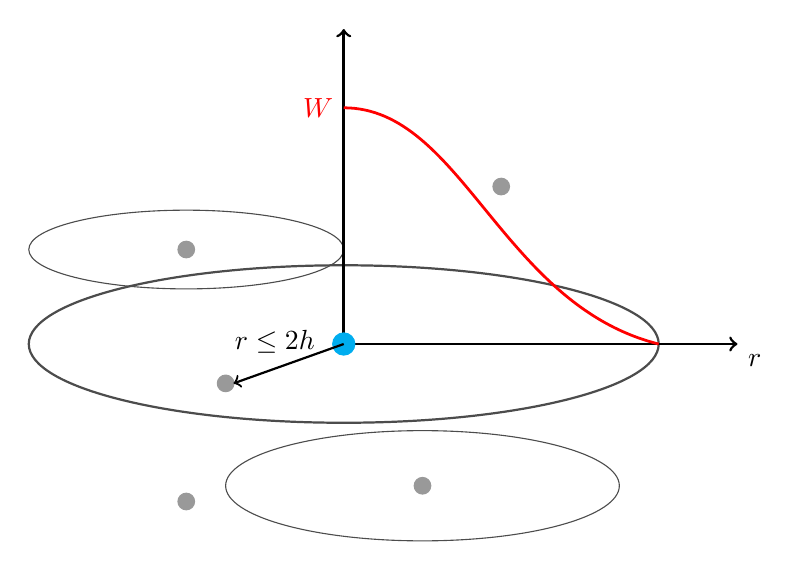
\begin{tikzpicture}
	
	% Others and their ellipse
	\draw [fill,black!40] (.5,1.5) circle (.3em);
	\draw [fill,black!40] (0,0) circle (.3em);
	\draw [fill,black!40] (0,3.2) circle (.3em);
	\draw[black!70] (0,3.2) ellipse (2 and .5);
	\draw [fill,black!40] (3,.2) circle (.3em);
	\draw[black!70] (3,.2) ellipse (2.5 and .7);
	\draw [fill,black!40] (4,4) circle (.3em);
	% Ellipses 
	\draw[line width=.8pt,black!70] (2,2) ellipse (4 and 1);
	% Axes
	\draw[->,line width=1pt] (2,2) -- (7,2) node[anchor=north west] {$r$};
	\draw[->,line width=1pt] (2,2) -- (2,6);
	% bezier for kernel 
	\draw[red,line width=1pt]  (6,2) .. controls (4,2.5) and (3.5,5) .. (2,5) node[red,anchor=east] {$W$};
	% main particle, at the end to cover
	\draw [fill,cyan] (2,2) circle (.4em);
	% Arrows 
	\draw[->,line width=.8pt] (2,2) -- (.6,1.5) node[midway, above,xshift=-.5em] {$r\leq2h$};
\end{tikzpicture}
%\includegraphics[scale=.4]{\locpath/figures/flecsph/sph.pdf}
\caption{SPH kernel $W$ and smoothing length $h$ representation}
\label{fig:sph_base}
\end{figure}

The method, as illustrated in Fig.~\ref{fig:sph_base}, computes the evolution of physical quantities for every particle regarding its neighbors in the radius of its smoothing length $h$. 
The particles in this radius are then valued according to their distance using a smoothing function $W$, also called a kernel. 
The fundamental SPH formulation for any physical quantity $A$ is then to compute with all the neighbors of $b$ of a particle by:
\begin{equation}
A(\vec{r}) \simeq \sum_b \frac{m_b}{\rho_b} A(\vec{r}_b) W ( |\vec{r}-\vec{r}_b|,h)
\end{equation}

On a physics aspect, this method has several advantages:
It can handle deformations, low densities, vacuum, and makes particle tracking easier. 
It also conserves mass, linear and angular momenta, and energy by its construction that implies independence of the numerical resolution. 
Another strong benefit of using SPH is its exact advection of fluid properties. 
Furthermore, the particle structure of SPH easily combines with tree methods for solving Newtonian gravity through N-body simulations.
As a mesh-free method, it avoids the need of grid to calculate the spatial derivatives. 

However, there are cons to consider using SPH: 
It is restricted to low-order rate of convergence on certain PDE formulations; 
It requires careful setup of initial distribution of particles; 
Further, it can be struggle to resolve turbulence-dominated flows and special care must be taken when handling high gradients such as shocks and surface structure of neutron stars.
Many works are leading to handle more cases and to push the limitations of this method \cite{dai2017dual,lind2016incompressible,ren2016dual}.

In this work, we are solving Lagrangian conservation equations (Euler equations) for mass, energy and momentum of an ideal fluid ~\cite{Landau1959}  such that:
\begin{equation}
\frac{d \rho}{d t} = - \rho \nabla \cdot \vec{v}, \quad
\frac{d u}{d t} = \left( \frac{P}{\rho^2} \right) \frac{d \rho}{d t}, \quad
\frac{d \vec{v}}{d t} = - \frac{\nabla P}{\rho}
\end{equation}
with $\rho$ the density, $P$ the pressure, $u$ the internal energy and $v$ the velocity, where $d/dt = \partial_t + \vec{v} \cdot \nabla$ which is convective derivative.

By using the volume element $V_b = m_b / \rho_b$, we can formulate the Newtonian SPH scheme~\cite{rosswog2009} such that
\begin{equation}
\label{eq:rho}
\rho_a = \sum_b m_b W_{ab} (h_a)
\end{equation}
\begin{equation}
\frac{d u_a}{dt} = \frac{P_a}{\rho_a^2} \sum_b m_b \vec{v}_{ab} \cdot \nabla_a W_{ab} 
\end{equation}
\begin{equation}
\frac{d \vec{v}_a}{d t} = - \sum_b m_b \left(\frac{P_a}{\rho_a^2} + \frac{P_b}{\rho_b^2} \right) \nabla_a W_{ab}
\end{equation}
where $W_{ab} = W(| \vec{r}_a - \vec{r}_b |,h)$ is the smoothing kernel. 
The equations we would like to solve allow for emergence of discontinuities from smooth initial data. 
At discontinuities, the entropy increases in shocks. That dissipation occurs inside the shock-front. 
The SPH formulation here is inviscid so we need to handle this dissipation near shocks. 
There are a number of way to handle this problem, but the most widespread approach is to add artificial viscosity (or artificial dissipation) terms in SPH formulation such that:
\begin{equation}
\left(\frac{d u_a}{dt} \right)_{art} = \frac{1}{2} \sum_b m_b \Pi_{ab} \vec{v}_{ab} \cdot \nabla_a W_{ab}
\end{equation}
\begin{equation}
\left(\frac{d\vec{v}_a}{dt} \right)_{art} = - \sum_b m_b \Pi_{ab}\nabla_a W_{ab}
\end{equation}
In general, we can express the equations for internal energy and acceleration with artificial viscosity
\begin{equation}
\label{eq:intern}
\frac{d u_a}{dt} = \sum_b m_b \left(\frac{P_a}{\rho_a^2} + \frac{\Pi_{ab}}{2} \right) \vec{v}_{ab} \cdot \nabla_a W_{ab}
\end{equation}
\begin{equation}
\label{eq:velo}
\frac{d \vec{v}_a}{d t} = - \sum_b m_b \left(\frac{P_a}{\rho_a^2} + \frac{P_b}{\rho_b^2} + \Pi_{ab} \right) \nabla_a W_{ab}
\end{equation}
$\Pi_{ab}$ is the artificial viscosity tensor. 
As long as $\Pi_{ab}$ is symmetric, the conservation of energy, linear and angular momentum is assured by the form of the equation and antisymmetry of the gradient of kernel with respect to the exchange of indices $a$ and $b$. $\Pi_{ab}$ may define different way but here we use~\cite{Monaghan1983} such as: 
\begin{equation}
\Pi_{ab} = \begin{cases}
\frac{- \alpha \bar{c}_{ab} \mu_{ab} + \beta \mu_{ab}^2}{\bar{\rho}_{ab}} & \text{for $\vec{r}_{ab} \cdot \vec{v}_{ab} < 0$} \\
0 & \text{otherwise}
\end{cases}
\end{equation}
\begin{equation}
\mu_{ab} = \frac{\bar{h}_{ab} \vec{r}_{ab} \cdot \vec{v}_{ab}}{r^2_{ab} + \epsilon \bar{h}_{ab}^2}
\end{equation}

Using the usual form $c_s$ as $c_s = \sqrt{\frac{\partial p}{\partial \rho}}$.
The values of $\epsilon$, $\alpha$, and $\beta$ have to be set regarding the problem targeted. 
Here, we use $\epsilon = 0.01h^2$, $\alpha = 1.0$, and $\beta = 2.0$. 

There are many possibilities for the smoothing function, called the kernel. 
As an example the Monaghan's cubic spline kernel is given by:
\begin{equation}
W(\vec{r},h) = \frac{\sigma}{h^D} \begin{cases}
1-\frac{3}{2} q^2 + \frac{3}{4} & \text{if} \indent 0 \leq q \leq 1 \\
\frac{1}{4} (1-q)^3  & \text{if} \indent 1 \leq q \leq 2 \\
0 & \text{otherwise}
\end{cases}
\end{equation}
where $q = r/h$, $r$ the distance between the two particles, $D$ is the number of dimensions and $\sigma$ is a normalization constant with the values:
\begin{equation}
\sigma =  \begin{cases}
\frac{2}{3} & \text{for 1D}  \\
\frac{10}{7 \pi} & \text{for 2D} \\
\frac{1}{\pi} & \text{for 3D}
\end{cases}
\end{equation}

To sum up, the SPH resolution scheme and its routines are presented on algorithm \ref{alg:sph}.
The Equation of State (EOS) and the integration are problem dependent and will be define for each test case in section \ref{sec:applications}. 

\begin{algorithm}
\caption{SPH loop algorithm}\label{alg:sph}
\begin{algorithmic}[1]
\While{not last step}
\State Compute density for each particle (\ref{eq:rho})
\State Compute pressure using EOS 
\State Compute acceleration from pressure forces (\ref{eq:velo})
\State Compute change of internal energy for acceleration (\ref{eq:intern})
\State Advance particles after integration
\EndWhile
\end{algorithmic}
\end{algorithm}

The main downside for the implementation of this method is the requirement for local computation on every particle. 
The particles have to be grouped locally to perform the computation of (\ref{eq:rho}), (\ref{eq:intern}) and (\ref{eq:velo}).
A communication step is needed before and after (\ref{eq:rho}) to get the local physical data to be able to compute (\ref{eq:intern}) and (\ref{eq:velo}).
The tree data structure allows us to perform $O(Nlog(N))$ neighbor search but also add a domain decomposition and distribution layer.

As the SPH method is used in a large panel of fields from astrophysics to fluid mechanic, there are numerous related works. 
We can cite a code developed in the LANL, 2HOT \cite{warren20132hot} that introduced the Hashed Oct Tree structure used in our implementation. 
There is also GADGET-2 \cite{springel2005cosmological}, GIZMO \cite{hopkins2014gizmo} and the most recent publication is GASOLINE \cite{wadsley2017gasoline2} based on PKDGRAV, a specific tree+gravity implementation. 
Several implementations already implement GPU code and tree construction and traversal, one can cite GOTHIC \cite{miki2017gothic}, presenting gravitational tree code accelerated using the latest Fermi, Kepler and Maxwell architectures. But a lot of GPU accelerated work still focused on fluid problems and not on astrophysical problems  \cite{harada2007smoothed,crespo2011gpus}.
We also note that these implementations focus on SPH problems and does not provide a general purpose and multi-physics framework like we intent to provide through FleCSPH and FleCSI. 

\subsection{Gravitation}
For classical problems like fluid flow the gravitation can directly be applied on the particles with the force:
\begin{equation}
	\vec{a_g} = m\vec{g}
\end{equation}

In order to consider astrophysics problems we need to introduice self-gravitation. 
Each particle imply an action on the others base on its distance and mass. 
The equation of gravitation for a particle $i$ with $j$ other particles is: 
\begin{equation}
	\vec{f_a}_i = \sum_j -G \frac{m_i m_j}{|\vec{r_i}-\vec{r_j}|^3} \vec{r_{ij}}
	\label{eq:gravitation}
\end{equation}

This computation involve an $O(N^2)$ complexity and thus is not applicable directly. 
We applied the method called Fast Multipole Method, FMM and discussed in \cite{beatson1997short}.
In this method we compute the gravitation up a approximations. 
The user can refine those approximation changing parameters. 

\begin{figure}
\resizebox {\columnwidth} {!} {
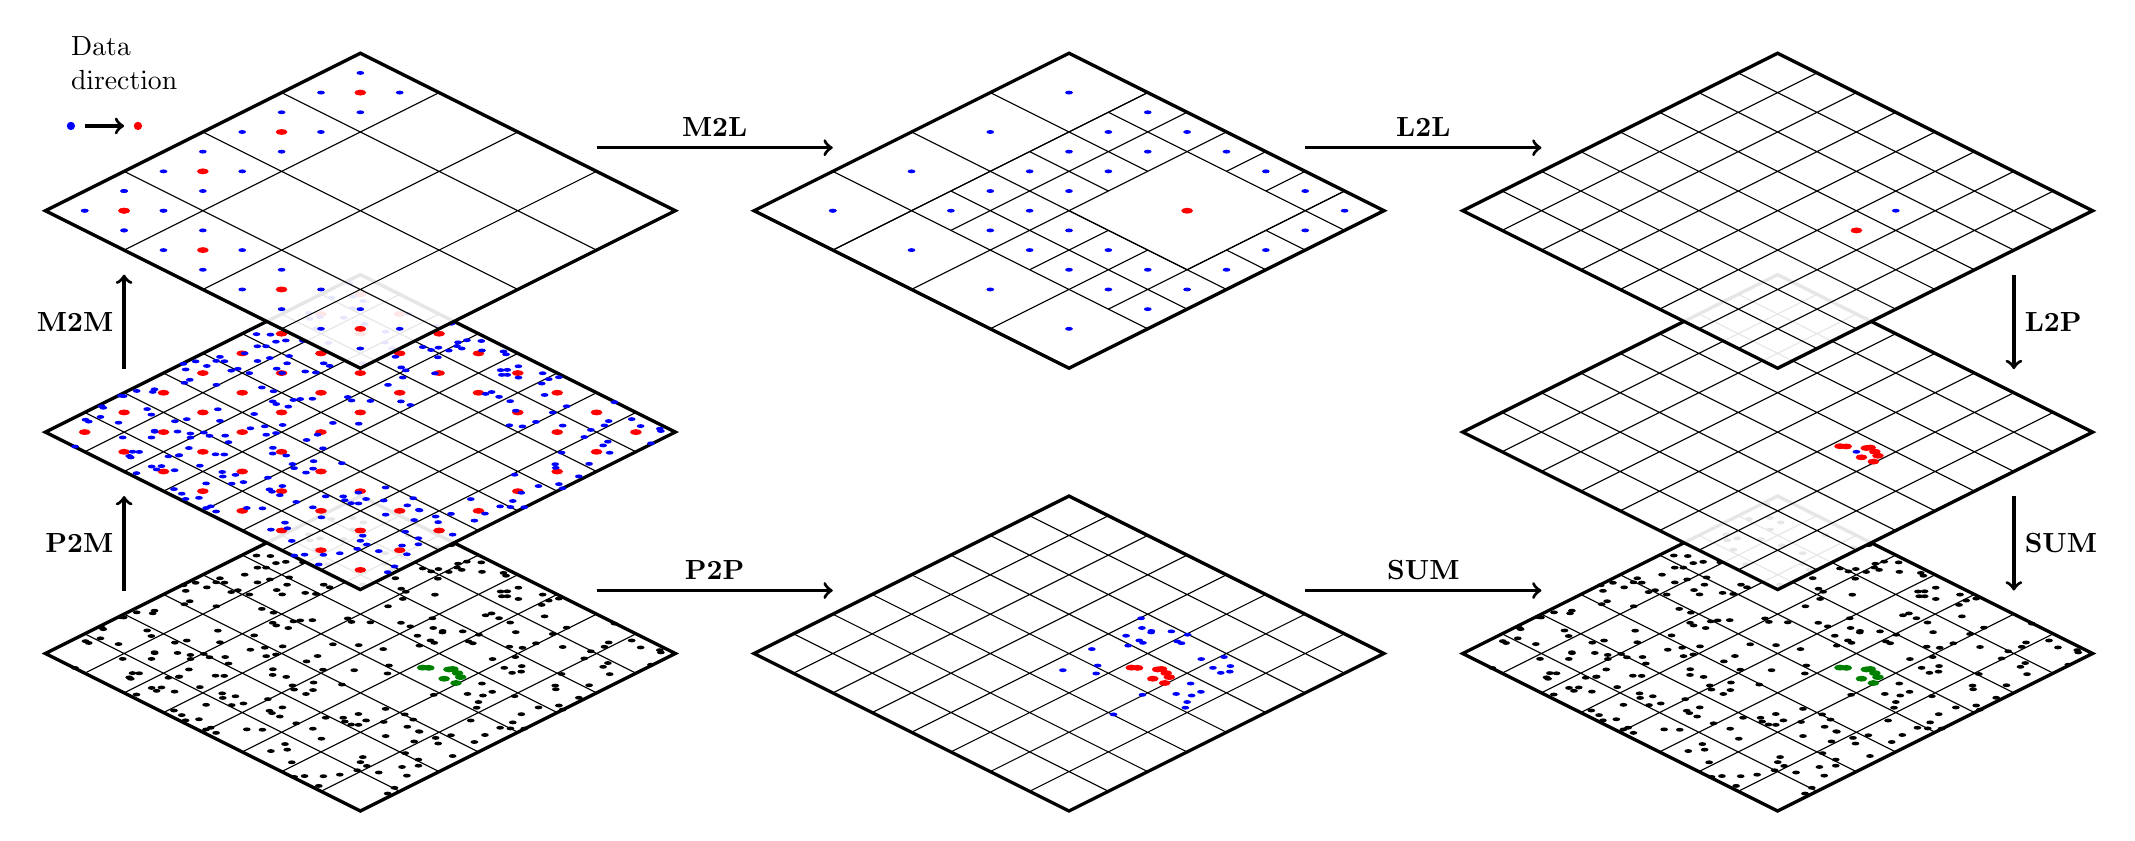
\begin{tikzpicture}
\def\nrand{300}
\def\seed{12}
\def\gridSize{5mm}
\def\gridTotal{4}
% Particles to Multipole
\pgfmathsetseed{\seed}
\begin{scope}[
   		yshift=0,every node/.append style={
    		yslant=0.5,xslant=-1},yslant=0.5,xslant=-1
    ]
    \fill[white,fill opacity=.9] (0,0) rectangle (4,4);
    \draw[black,very thick] (0,0) rectangle (4,4);
	\draw[step=\gridSize, black] (0,0) grid (\gridTotal,\gridTotal);
	\foreach \i in {1,2,...,\nrand}{
    	\pgfmathsetmacro{\x}{(rand)*2+2}
    	\pgfmathsetmacro{\y}{(rand)*2+2}
		% COLOR 
		\ifthenelse{\( \lengthtest{\x cm>2cm} \AND \lengthtest{\x cm<2.5cm} \)}
		{	
			\ifthenelse{ \( \lengthtest{\y cm>1cm} \AND \lengthtest{\y cm<1.5cm} \)}
			{\node at (\x,\y) [black!50!green,circle,fill,inner sep=.7pt,minimum size=3pt]{};}
			{\node at (\x,\y) [circle,fill,inner sep=.7pt]{};}
		}
		{\node at (\x,\y) [circle,fill,inner sep=.7pt]{};}
	}
\end{scope}
\pgfmathsetseed{\seed}
\begin{scope}[
   		yshift=80,every node/.append style={
    		yslant=0.5,xslant=-1},yslant=0.5,xslant=-1
    ]
    \fill[white,fill opacity=.9] (0,0) rectangle (4,4);
    \draw[black,very thick] (0,0) rectangle (4,4);
	\draw[step=5mm, black] (0,0) grid (\gridTotal,\gridTotal);
	\foreach \x in {0,1,...,7}{\foreach \y in {0,1,...,7}{
		\ifthenelse{\( \x<3 \OR \x>5 \)}
		{
			\node at (\x*\gridSize+\gridSize/2,\y*\gridSize+\gridSize/2)[red,circle,fill,inner sep=.7pt,minimum size=3pt]{};
		}
		{	\ifthenelse{ \( \y<1 \OR \y>3 \)}
			{
			\node at (\x*\gridSize+\gridSize/2,\y*\gridSize+\gridSize/2)[red,circle,fill,inner sep=.7pt,minimum size=3pt]{};	
			}{}
		}
	}}
	\foreach \i in {1,2,...,\nrand}{
    	\pgfmathsetmacro{\x}{(rand)*2+2}
    	\pgfmathsetmacro{\y}{(rand)*2+2}
    	\ifthenelse{\( \lengthtest{\x cm<1.5cm} \OR \lengthtest{\x cm>3cm} \)}
		{\node at (\x,\y) [blue,circle,fill,inner sep=.7pt]{};}
		{	\ifthenelse{ \( \lengthtest{\y cm<.5cm} \OR \lengthtest{\y cm>2cm} \)}
			{\node at (\x,\y) [blue,circle,fill,inner sep=.7pt]{};}
			{}
		}
  	}
\end{scope}
\begin{scope}[
   		yshift=160,every node/.append style={
    		yslant=0.5,xslant=-1},yslant=0.5,xslant=-1
    ]
    \fill[white,fill opacity=.9] (0,0) rectangle (4,4);
    \draw[black,very thick] (0,0) rectangle (4,4);
	\draw[step=10mm, black] (0,0) grid (4,4);
	\foreach \x in {0,1}{\foreach \y in {0,...,7}{
		\node at (\x*\gridSize+\gridSize/2,\y*\gridSize+\gridSize/2)[blue,circle,fill,inner sep=.7pt]{};
	}}
	\foreach \x in {0,...,7}{\foreach \y in {6,7}{
		\node at (\x*\gridSize+\gridSize/2,\y*\gridSize+\gridSize/2)[blue,circle,fill,inner sep=.7pt]{};
	}}

	\foreach \x in {0}{\foreach \y in {0,...,3}{				  
		\node at (\x*\gridSize*2+\gridSize,\y*\gridSize*2+\gridSize) [red,circle,fill,inner sep=.7pt,minimum size=3pt]{};
	}}
	\foreach \x in {0,...,3}{\foreach \y in {3}{				  
		\node at (\x*\gridSize*2+\gridSize,\y*\gridSize*2+\gridSize) [red,circle,fill,inner sep=.7pt,minimum size=3pt]{};
	}}
\end{scope}

%PARTICLES TO PARTICLES
\pgfmathsetseed{\seed}
\begin{scope}[
   		yshift=0,xshift=9cm,every node/.append style={
    		yslant=0.5,xslant=-1},yslant=0.5,xslant=-1
    ]
    \fill[white,fill opacity=.9] (0,0) rectangle (4,4);
    \draw[black,very thick] (0,0) rectangle (4,4);
	\draw[step=5mm, black] (0,0) grid (4,4);
	\foreach \i in {1,2,...,\nrand}{
    	\pgfmathsetmacro{\x}{(rand)*2+2}
    	\pgfmathsetmacro{\y}{(rand)*2+2}
    	\ifthenelse{\( \lengthtest{\x cm>1.5cm} \AND \lengthtest{\x cm<3cm} \)}
		{	
			\ifthenelse{ \( \lengthtest{\y cm>.5cm} \AND \lengthtest{\y cm<2cm} \)}
			{
				% COLOR 
				\ifthenelse{\( \lengthtest{\x cm>2cm} \AND \lengthtest{\x cm<2.5cm} \)}
				{	
					\ifthenelse{ \( \lengthtest{\y cm>1cm} \AND \lengthtest{\y cm<1.5cm} \)}
					{\node at (\x,\y) [red,circle,fill,inner sep=.7pt,minimum size=3pt]{};}
					{\node at (\x,\y) [blue,circle,fill,inner sep=.7pt]{};}
				}
				{\node at (\x,\y) [blue,circle,fill,inner sep=.7pt]{};}
			}{}
		}{}
    	%\node at (\x,\y) [circle,fill,inner sep=.7pt]{};
  	}
\end{scope}
%MULTIPOLE TO MULTIPOLE
\begin{scope}[
   		yshift=160,xshift=9cm,every node/.append style={
    		yslant=0.5,xslant=-1},yslant=0.5,xslant=-1
    ]
    \fill[white,fill opacity=.9] (0,0) rectangle (4,4);
    \draw[black,very thick] (0,0) rectangle (4,4);
    \draw[step=10mm, black] (0,3) grid (4,4);
	\draw[step=10mm, black] (0,0) grid (1,3);
	\draw[step=5mm, black] (1,0) grid (2,3);
	\draw[step=5mm, black] (2,2) grid (4,3);
	\draw[step=5mm, black] (2,0) grid (4,.5);
	\draw[step=5mm, black] (3.5,0) grid (4,2);
	% add rectangle
	\draw[black] (2,.5) rectangle (3.5,2);
	% Big part 
	\foreach \x in {0}{\foreach \y in {0,...,3}{				  
		\node at (\x*\gridSize*2+\gridSize,\y*\gridSize*2+\gridSize) [blue,circle,fill,inner sep=.7pt]{};
	}}
	\foreach \x in {0,...,3}{\foreach \y in {3}{				  
		\node at (\x*\gridSize*2+\gridSize,\y*\gridSize*2+\gridSize) [blue,circle,fill,inner sep=.7pt]{};
	}}
	% Smaller one 
	\foreach \x in {2,3}{\foreach \y in {0,...,3}{
		\node at (\x*\gridSize+\gridSize/2,\y*\gridSize+\gridSize/2)[blue,circle,fill,inner sep=.7pt]{};
	}}

	\foreach \x in {2,...,7}{\foreach \y in {4,5}{
		\node at (\x*\gridSize+\gridSize/2,\y*\gridSize+\gridSize/2)[blue,circle,fill,inner sep=.7pt]{};
	}}

	\foreach \x in {7}{\foreach \y in {0,...,3}{
		\node at (\x*\gridSize+\gridSize/2,\y*\gridSize+\gridSize/2)[blue,circle,fill,inner sep=.7pt]{};
	}}
	\foreach \x in {4,5,6}{\foreach \y in {0}{
		\node at (\x*\gridSize+\gridSize/2,\y*\gridSize+\gridSize/2)[blue,circle,fill,inner sep=.7pt]{};
	}}
	\node at (5*\gridSize+\gridSize/2,2*\gridSize+\gridSize/2) [red,circle,fill,inner sep=.7pt,minimum size=3pt]{};
\end{scope}

% Multipole to Particles 
\pgfmathsetseed{\seed}
\begin{scope}[
   		yshift=0,xshift=18cm,every node/.append style={
    		yslant=0.5,xslant=-1},yslant=0.5,xslant=-1
    ]
    \fill[white,fill opacity=.9] (0,0) rectangle (4,4);
    \draw[black,very thick] (0,0) rectangle (4,4);
	\draw[step=5mm, black] (0,0) grid (4,4);
	\foreach \i in {1,2,...,\nrand}{
    	\pgfmathsetmacro{\x}{(rand)*2+2}
    	\pgfmathsetmacro{\y}{(rand)*2+2}
		% COLOR 
		\ifthenelse{\( \lengthtest{\x cm>2cm} \AND \lengthtest{\x cm<2.5cm} \)}
		{	
			\ifthenelse{ \( \lengthtest{\y cm>1cm} \AND \lengthtest{\y cm<1.5cm} \)}
			{\node at (\x,\y) [black!50!green,circle,fill,inner sep=.7pt,minimum size=3pt]{};}
			{\node at (\x,\y) [circle,fill,inner sep=.7pt]{};}
		}
		{\node at (\x,\y) [circle,fill,inner sep=.7pt]{};}
	}
\end{scope}
\pgfmathsetseed{\seed}
\begin{scope}[
   		yshift=80,xshift=18cm,every node/.append style={
    		yslant=0.5,xslant=-1},yslant=0.5,xslant=-1
    ]
    \fill[white,fill opacity=.9] (0,0) rectangle (4,4);
    \draw[black,very thick] (0,0) rectangle (4,4);
	\draw[step=5mm, black] (0,0) grid (4,4);

	\foreach \i in {1,2,...,\nrand}{
    	\pgfmathsetmacro{\x}{(rand)*2+2}
    	\pgfmathsetmacro{\y}{(rand)*2+2}
    	\ifthenelse{\( \lengthtest{\x cm>1.5cm} \AND \lengthtest{\x cm<3cm} \)}
		{	
			\ifthenelse{ \( \lengthtest{\y cm>.5cm} \AND \lengthtest{\y cm<2cm} \)}
			{
				% COLOR 
				\ifthenelse{\( \lengthtest{\x cm>2cm} \AND \lengthtest{\x cm<2.5cm} \)}
				{	
					\ifthenelse{ \( \lengthtest{\y cm>1cm} \AND \lengthtest{\y cm<1.5cm} \)}
					{\node at (\x,\y) [red,circle,fill,inner sep=.7pt,minimum size=3pt]{};}
					{}
				}{}
			}{}
		}{}
	}
	\node at (4*\gridSize+\gridSize/2,2*\gridSize+\gridSize/2) [blue,circle,fill,inner sep=.7pt]{};
\end{scope}
%% MULTIPOLE TO LOCAL
\begin{scope}[
   		yshift=160,xshift=18cm,every node/.append style={
    		yslant=0.5,xslant=-1},yslant=0.5,xslant=-1
    ]
    \fill[white,fill opacity=.9] (0,0) rectangle (4,4);
    \draw[black,very thick] (0,0) rectangle (4,4);
	\draw[step=5mm, black] (0,0) grid (4,4);
	\node at (4*\gridSize+\gridSize/2,2*\gridSize+\gridSize/2) [red,circle,fill,inner sep=.7pt,minimum size=3pt]{};

	\node at (5*\gridSize+\gridSize/2,2*\gridSize+\gridSize/2) [blue,circle,fill,inner sep=.7pt]{};
\end{scope}
% ARROWS AND TEXT
\draw[->,very thick] (-3,2.8) -- (-3,4) node[midway,left] {\textbf{P2M}};
\draw[->,very thick] ([yshift=80]-3,2.8) -- ([yshift=80]-3,4) node[midway,left] {\textbf{M2M}};

\draw[->,very thick] ([yshift=160]3,2.8) -- ([yshift=160]6,2.8) node[midway,above] {\textbf{M2L}};
\draw[->,very thick] ([yshift=160,xshift=9cm]3,2.8) -- ([yshift=160,xshift=9cm]6,2.8) node[midway,above] {\textbf{L2L}};

\draw[<-,very thick] ([yshift=80]21,2.8) -- ([yshift=80]21,4) node[midway,right] {\textbf{L2P}};
\draw[<-,very thick] (21,2.8) -- (21,4) node[midway,right] {\textbf{SUM}};

\draw[->,very thick] (3,2.8) -- (6,2.8) node[midway,above] {\textbf{P2P}};
\draw[->,very thick] ([xshift=9cm]3,2.8) -- ([xshift=9cm]6,2.8) node[midway,above] {\textbf{SUM}};


\draw[->,very thick] (-3.5,8.7cm) node[xshift=-5pt,blue,circle,fill,inner sep=.7pt,minimum size=3pt] (a) {} -- 
 (-3,8.7cm) node[xshift=5pt,red,circle,fill,inner sep=.7pt,minimum size=3pt] (b) {};
\node[align=left] at (-3,9.5cm) {Data\\direction};


\end{tikzpicture}
}
\caption{Fast Multipole Method schematics. Particles to Multipole (P2M), Multipole to Multipole (M2M), Multipole to Particles (M2P), Multipole to Local (M2L), Local to Local (L2L) and Particles to Particles (P2P). Schematic inspired from \cite{yokota2011treecode}}
\end{figure}

This method is based on Taylor series.
The gravitation function of equation~\ref{eq:gravitation} can be approximate on a particle at position $\vec{r}$ by the gravitation computed at the centroid at position $\vec{r_c}$: 
\begin{equation}
 \vec{f}(\vec{r}) = \vec{f}(\vec{r_c}) + ||\frac{\partial\vec{f}}{\partial\vec{r}}||\cdot (\vec{r} - \vec{r_c}) + \frac{1}{2} (\vec{r}-\vec{r_c})^\intercal \cdot   ||\frac{\partial\vec{f}}{\partial\vec{r} \partial\vec{r}}|| \cdot (\vec{r} - \vec{r_c})
 \end{equation}

 From equation~\ref{eq:gravitation} we compute the term $||\frac{\partial\vec{f}}{\partial\vec{r}}||$:s
 \begin{equation}
\frac{\partial\vec{f}}{\partial\vec{r}} =
- \sum_p \frac{m_p}{|\vec{r_c}-\vec{r_p}|^3}
\begin{bmatrix}
1 - \frac{3(x_c-x_p)(x_c-x_p)}{|\overline{r_c}-\overline{r_p}|^2} & -\frac{3(y_c-y_p)(x_c-x_p)}{|\overline{r_c}-\overline{r_p}|^2}  & -\frac{3(z_c-z_p)(x_c-x_p)}{|\vec{r_c}-\vec{r_p}|^2}  \\
-\frac{3(x_c-x_p)(y_c-y_p)}{|\vec{r_c}-\vec{r_p}|^2}  & 1 - \frac{3(y_c-y_p)(y_c-y_p)}{|\vec{r_c}-\vec{r_p}|^2} &  -\frac{3(z_c-z_p)(y_c-y_p)}{|\vec{r_c}-\vec{r_p}|^2}\\
- \frac{3(x_c-x_p)(z_c-z_p)}{|\vec{r_c}-\vec{r_p}|^2}   &  -\frac{3(y_c-y_p)(z_c-z_p)}{|\vec{r_c}-\vec{r_p}|^2} &  1- \frac{3(z_c-z_p)(z_c-z_p)}{|\vec{r_c}-\vec{r_p}|^2} \\
\end{bmatrix}
 \end{equation}

And we propose a compact version of the matrix with: 
 
\begin{equation}
 ||\frac{\partial f^a}{\partial r^b}|| = -\sum_c \frac{m_c}{|\vec{r}-\vec{r_c}|^3} \Big[ \delta_{ab} - \frac{3.(r^a-r_c^a)(r^b-r_c^b)}{|\vec{r}-\vec{r_c}|^2} \Big] 
\end{equation}

With $\delta_{ab}$ the kronecker delta:
\begin{equation}
\delta_{ab} = 
\begin{cases}
    1, & \text{if $a = b$}.\\
    0, & \text{if $a\neq b$}.
  \end{cases}
\end{equation}

We note that $a$ and $b$ variate from 0 to 2 and $r^0=x$, $r^1=y$, and $r^2=z$ as usual sense. 

For the term $||\frac{\partial\vec{f}}{\partial\vec{r} \partial\vec{r}}||$ we give the compact version by:
\begin{equation}
||\frac{\partial^2 f^a}{\partial r^b \partial r^c}|| =
- \sum_c \frac{3 m_c}{|\vec{r}-\vec{r_c}|^5} \left[\frac{5(r^a-r_c^a)(r^b-r_c^b)(r^c-r_c^c)}{|\vec{r}-\vec{r_c}|^2} - \left( \delta_{ab} (r^c-r_c^c)+\delta_{bc} (r^a-r_c^a)+\delta_{ac} (r^b-r_c^b) \right) \right] 
 \end{equation} 

 \begin{figure}
 \end{figure}

The method is summed up in figure with the different equations.
We consider Centers Of Mass, COM, to be the centroid of particles based on their position. 
In several steps the information is first transmitted to the COMs, computing their position and mass. 


\subsection{Problems} 
The previous equations are generic and describe the behavior of SPH method. 
In order to check our 

\subsubsection{Sod shock tube}

\subsubsection{Sedov blast wave}

\subsubsection{Fluid flow}

\subsubsection{Astrophysics: neutron stars coalescence}

The final aim of our tests is to simulate astrophysical events. 
We are interested in one of the most important event recently discovered. 
Last year the Laser Interferometer Gravitational Wave, LIGO, detected the first gravitational wave generated by binary neutron stars merging \cite{abbott2017gw170817} and also more complexes event with Binary Black Holes coalescence in \cite{abbott2017gw170814}.


\paragraph{Solving Lane-Emden Equation}

We need to determine the density function based on the radius. 

As we consider the star as a polytropic fluid, we use the equation of Lane-Emden which is a form of the Poisson equation: 

\begin{equation}\label{eq_LaneEmden}
  \frac{d^2\theta}{d \xi^2}+ \frac{2}{\xi}\frac{d\theta}{d\xi}+\theta^n = 0
\end{equation}

With $\xi$ and $\theta$ two dimensionless variables. 
There is only exact solutions for a polytropic index $n = 0.5$, $1$ and $2$.
In our work we use a polytropic index of $1$ which can correspond to a NS simulation.

For $n=1$ the solution of equation \ref{eq_LaneEmden} is: 

\begin{equation}
\theta(\xi)=\frac{sin(\xi)}{\xi}
\end{equation}

We note $\xi_1 = \pi$, the first value of $\xi$ as $\theta(\xi) = 0$.
$\theta(\xi)$ is also defined as: 
\begin{equation}
 \theta(\xi) = \Big(\frac{\rho(\xi)}{\rho_c}\Big)^{\frac{1}{n}}  = \frac{\rho(\xi)}{\rho_c}
\end{equation}

With $\rho_c$ the internal density of the star and $\rho$ the density at a determined radius. $\xi$ is defined as:  
$$ \xi = Ar = \sqrt{\frac{4\pi G}{K(n+1)}\rho_c^{(n-1)/n}} \times r = \sqrt{\frac{2\pi G}{K}}\times r \mbox{ (for } n=1 \mbox{)}$$

With $K$ a proportionality constant.

From the previous equations we can write the stellar radius $R$ as:
\begin{equation}
R = \sqrt{\frac{K(n+1)}{4\pi G}}\rho_c^{(1-n)/2}\xi_1 = \sqrt{ \frac{K}{2\pi G} } \times \xi_1
\end{equation} 

(We note that for $n=1$ the radius does not depend of the central density.)

If, for example, we use dimensionless units as $G=R=M=1$ (for the other results we use CGS with $G = 6.674 \times 10^{-8} cm^3g^{-1}s^{-2}$) 
We can compute K as: 
\begin{equation}
\label{eq:constant}
K = \frac{R^2  2 \pi G}{\xi_1^2}
\end{equation}

\begin{center}

\begin{tabular}{c|c|c|c|c|}
 & $NS_1$ & $NS_2$ & $NS_3$ & $NS_4$ \\ 
\hline 
Radius (cm) & $R=G=M=1$ & 1500000 & 1400000 & 960000 \\ 
\hline 
K & 0.636619 & 95598.00 & 83576.48 & 39156.94\\ 
\hline 
\end{tabular}

\end{center} 

Then we deduce the density function of $r$ as :

$$\rho(\xi) = \frac{sin(A\times r)}{A \times r} \times \rho_c \mbox{ with } A = \sqrt{\frac{2\pi G}{K}}
$$

As we know the total Mass $M$, the radius $R$ and the gravitational constant $G$ we can compute the central density as: 

$$ \rho_c = \frac{M A^3}{4 \pi (sin(AR)-ARcos(AR)) } $$

Then we normalize the results to fit $R = M = G = 1$: $K' = K/(R^2G) $, $m_i' = m_i/M $, $h_i' = h_i / R$, $\vec{x_i}' = \vec{x_i}/R$ 

\section{Conclusion}



%%%%%%%%%%%%%%%%%%%%%%%%%%%%%%%%%%%%%%%%%%%%%%%%%%%%%%%%%%%%%%%%%%%%%
%																	%
%	CHAPTER TWO, HARDWARE IN HPV									%
%																	%
%%%%%%%%%%%%%%%%%%%%%%%%%%%%%%%%%%%%%%%%%%%%%%%%%%%%%%%%%%%%%%%%%%%%%
%%%%%%%%%%%%%%%%%%%%%%%%%%%%%%%%%%%%%%%%%%%%%%%%%%%%%%%%%%%%%%%%%%%%%
%                                                                   %
% CHAPTER FIVE: COMPUTATIONAL WALL: LANGFORD PROBLEM                %
%                                                                   %
%%%%%%%%%%%%%%%%%%%%%%%%%%%%%%%%%%%%%%%%%%%%%%%%%%%%%%%%%%%%%%%%%%%%%

\chapter{Computational Wall: Langford Problem}

\section{Introduction}
Our aim is to determine the behavior of accelerators compared to classical processor in case of irregular-computationally heavy problems.
For this purpose we choose the Langford problem which is an academic problem of combinatorial counting.
We show the optimizations made to the regular processor algorithm to efficiently implement this application on GPU. 
We compare the two approaches from classical processor to GPU implementation. 
The results are then presented to show the acceleration using the whole ROMEO supercomputer.
This study shows two approaches to the Langford problem.
The Miller's algorithm, irregular tree backtracking and the the Godfrey's method which is use in order to beat a time record on this problem.\\

C. Dudley Langford gave his name to a classic permutation problem ~\cite{Gard56, Simp83}.  
While observing his son manipulating blocks of different colors, he noticed that it was possible to arrange three pairs of different colored blocks (yellow, red and blue) in such a way that only one block separates the red pair - noted as pair 1 - , two blocks separate the blue pair - noted as pair 2 - and finally three blocks separate the yellow one - noted as pair 3 - , see figure~\ref{fig:lang}.\\

\begin{figure}[htbp]    
\begin{center}    
%\includegraphics[scale=0.45]{\locpath/figures/langford/lgf_cubes}   
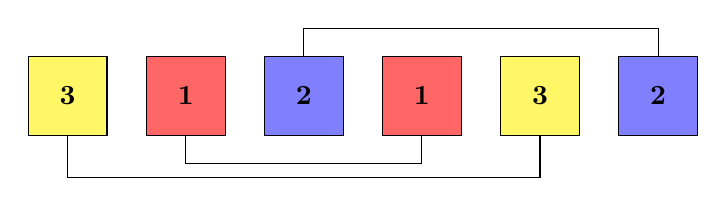
\begin{tikzpicture}
\node (rect) at (0,0) [fill=yellow!60,draw,minimum width=1cm,minimum height=1cm] (p3_1) {\textbf{3}};
\node (rect) at (1.5,0) [fill=red!60,draw,minimum width=1cm,minimum height=1cm] (p1_1) {\textbf{1}};
\node (rect) at (3,0) [fill=blue!50,draw,minimum width=1cm,minimum height=1cm] (p2_1) {\textbf{2}};
\node (rect) at (4.5,0) [fill=red!60,draw,minimum width=1cm,minimum height=1cm] (p1_2) {\textbf{1}};
\node (rect) at (6,0) [fill=yellow!60,draw,minimum width=1cm,minimum height=1cm] (p3_2) {\textbf{3}};
\node (rect) at (7.5,0) [fill=blue!50,draw,minimum width=1cm,minimum height=1cm] (p2_2) {\textbf{2}};
\draw (p3_1.south) -- ([yshift=-15pt]p3_1.south) -- ([yshift=-15pt]p3_2.south) -- (p3_2.south) ;
\draw (p2_1.north) -- ([yshift=10pt]p2_1.north) -- ([yshift=10pt]p2_2.north) -- (p2_2.north) ;
\draw (p1_1.south) -- ([yshift=-10pt]p1_1.south) -- ([yshift=-10pt]p1_2.south) -- (p1_2.south) ;
\end{tikzpicture}  
\end{center}
\caption{L(2,3) arrangement} \label{fig:lang}  
\end{figure}
  
This problem has been generalized to any number $n$ of colors and any number $s$ of blocks having the same color. 
$L(s,n)$ consists in searching for the number of solutions to the Langford problem, up to a symmetry. % ... excepted symmetric ones. 
In November 1967, Martin Gardner presented $L(2,4)$ (two cubes and four colors) as being part of a collection of small mathematical games and he stated that $L(2,n)$ has solutions for all $n$ such that:
\begin{equation}
\text{ solutions for: }
\begin{cases}
n= 4k \\ 
n = 4k-1
\end{cases}
 k \in \mathbb{N}^+
\end{equation}
The central resolution method consists in placing the pairs of cubes, one after the other, on the free places and backtracking if no place is available (see figure~\ref{backtrack} for detailed algorithm).

\begin{table}[t!]
\centering
\[
\begin{tabular}{c r r r}
  \hline
  Instance & Solutions & Method & Computation time\\
  \hline
  \hline
  L(2,3) & 1 &  Miller algorithm & - \\
  L(2,4) & 1 & & - \\ 
  ... & ... & & ...  \\
  L(2,16) & 326,721,800 & & 120 hours  \\
  %\cline{1-3}
  L(2,19) & 256,814,891,280 & & 2.5 years (1999) DEC Alpha \\
  \hline
  \hline
  L(2,20) & 2,636,337,861,200 & Godfrey algorithm & 1 week \\
  %\cline{1-3}
  L(2,23) & 3,799,455,942,515,488 & &  4 days with CONFIIT \\
  %\cline{1-3}
  L(2,24) & 46,845,158,056,515,936 & & 3 months with CONFIIT \\
  L(2,27) & 111,683,611,098,764,903,232 & & 2 days on ROMEO \\
  L(2,28) & 1,607,383,260,609,382,393,152 & & 23 days on ROMEO \\
  \hline
\end{tabular}
\]
\caption{Solutions and time for Langford problem using different methods}
\label{tab:result_base}
\end{table}

The Langford problem has been approached in different ways: discrete mathematics results, specific algorithms, specific encoding, constraint satisfaction problem (CSP), inclusion-exclusion~\ldots~\cite{Mil00,apes-26,Smi00,larsen2009counting}.
In 2004, the last solved instance, $L(2,24)$, was computed by our team \cite{CReSTIC-711} using a specific algorithm. 
Table \ref{tab:result_base} presents the latest results and number of solutions. 
$L(2,27)$ and $L(2,28)$ have just been computed but no details were given. 

The most efficient known algorithms are: the Miller backtrack method, the Godfrey algebraic method and the Larsen inclusion-exclusion method.
The Miller one is based on backtracking and can be modeled as a CSP; it allowed us to move the limit of explicits solutions building up to $L(2,21)$ but combinatorial explosion did not allow us to go further. 
Then, we use the Godfrey method to achieve $L(2,24)$ more quickly and then recompute $L(2,27)$ and $L(2,28)$, presently known as the last instances.
The Larsen method is based on inclusion-exclusion \cite{larsen2009counting}; although this method is effective, practically the Godfrey one is better. 
The latest known work on the Langford Problem is a GPU implementation proposed in \cite{ASS_LGF} in 2015. Unfortunately this study does not provide any performance considerations but just gives the number of solution of $L(2,27)$ and $L(2,28)$.

\section{Miller algorithm}

In this part we present our multi-GPU cluster implementation of the Miller's algorithm. 
This algorithm is very irregular and the repartition have to be done at runtime on our accelerators. 

First, we introduce the backtrack method. 
Then we present our implementation in order to fit the GPUs architecture. 
The last section presents our results. 

\subsection{CSP}

Combinatorial problems are NP-complete \cite{GJ79} and can be described as SATISFIABILITY problems (SAT) using a polynomial transformation. 
They can be transformed into CSP formalism.
A Constraint Satisfaction Problem (CSP), first introduced by Montanari \cite{Mon74}, is defined as a triple $<X,D,C>$ where:
\begin{equation}
\begin{cases}
X=\{X_1,...,X_n\}\text{: a finite set of variables} \\ 
D=\{D_1,...,D_n\}\text{: their finite domains of values}\\
C=\{C_1,...,C_p\}\text{: a finite set of constraints}
\end{cases}
\end{equation}

The goal in this formalism is to assign values in $D$ to $n$-uple $X$ respecting all the $C$ $p$-uple constraints.
This approach is a large field of research. \cite{arbelaez2014gpu} developed \textit{local search} and compares GPU to CPU. 
This first work brings to light that GPU is a real contributor to the global computation speed. \cite{campeotto2014exploring} proposes a solver using \textit{propagator} on a GPU architecture to solve CSP problems. 
\cite{jenkins2011lessons} cares about GPU weak points, loading bandwidth and global memory latency.

%\subsection{CSP parallel resolution}
%\label{sec:CSP_resolution}

Considering a basic approach, combinatorial problems formed into CSP can be represented as a tree search. Each level corresponds to a given variable, with values in its domain. Leaves of the tree correspond to a complete assignment (all variables are set). If it meets all the constraints this assignment is called an acceptor state. Depending on the constraints set, the satisfiability evaluation can be made either on complete or partial assignment.
%
%There are many ways to browse the tree and find the solutions: \emph{backtracking}, \emph{forward-checking}, \emph{backjumping}, etc. 
%We limit our method to the naive \emph{backtrack} resolution. We chose to evaluate the variables and their values in a static order; in a depth-first manner, the solution is built incrementally and if a partial assignment can be aborted, the branch is cut. A solution is found each time a leaf is reached.
%% presents a backtrack search with the previous CSP representation.
%
%The recommendation for performance on GPU accelerator is to use non test-based programs.
%Due to its irregularity, the basic \emph{backtracking} algorithm is suppose not to suit the GPU architecture.
%Thus a vectorized version is given when evaluating the assignments at the leaves' level, with one of the two following ways: assignments can be prepared on each tree node or totally set on final leaves before testing the satisfiability of the built solution, Fig.\ref{fig:algos}.
%
%\begin{figure}[htbf]
%\begin{minipage}[b]{0.45\linewidth}
%\begin{verbatim}
%for variable_1 
%   assignment
%   for variable_2
%      assignment
%      ...
%         for variable_n
%            assignment
%            test
%\end{verbatim}
%\end{minipage}
%\begin{minipage}[b]{0.45\linewidth}
%\begin{verbatim}
%for variable_1 
%   for variable_2
%   ...
%      for variable_n
%         assignments
%         test
%         
%         
%\end{verbatim}
%\end{minipage} 
%\caption{CSP regularized algorithms}
%\label{fig:algos}
%\end{figure} 
%
%With this method it is necessary to browse the entire tree but this requires using all the search space and it is too time-consuming.
%
%In order to overcome this we divide the work between CPU and GPU. The CPU generates some levels of the tree and creates tasks. Then GPU and CPU cores divide up the workload in order to achieve the generation on the latest levels of the tree. With this method, inconsistent branches can be cut on highest level and GPU/CPU cores only compute possibly consistent tasks.
%
%This representation enables a server-client model to distribute the tasks: the server generates independent sub-problems at a chosen depth in the tree, treated by clients. 
%Each client decomposes the sub-problem into tasks, distributed over the GPU/CPU cores, Fig.\ref{fig:parallel}.
%
%\begin{figure}[htbf]
%\centering 
%\includegraphics[scale=0.9]{figures/graphe_repartition}   
%\caption{Server client distribution} \label{fig:parallel}    
%\end{figure} 
%
%With this method numerous branches have been cut from the main tree during generation stage and GPU/CPU tasks are faster due to their lower depth. Despite the combinatorial explosion of this kind of problem, we can consider solving CSP in a massively parallel manner on multiGPU clusters.

\subsection{Backtrack resolution}

As presented above the Langford problem is known to be a highly irregular combinatorial problem. 
We first present here the general tree representation and the ways we regularize the computation for GPUs.
Then we show how to parallelize the resolution over a multi-GPU cluster.

\subsubsection{Langford's problem tree representation}
\label{sec:LGF_resolution}
%In~\cite{HKS02}, we propose to formalize the Langford problem as a CSP  ({\it Constraint Satisfaction Problem}), first introduced by Montanari in \cite{Mon74}, and show that an efficient parallel resolution is possible. 
As explained, CSP formalized problems can be transformed into tree evaluations. %represented as trees. 
%The tree Here we intend to develop a specific algorithm taking into account the conclusion of our previous studies (memory management of memory and load balance) and transfer the tasks resolution into GPUs.\\
%\begin{figure}[htb]
%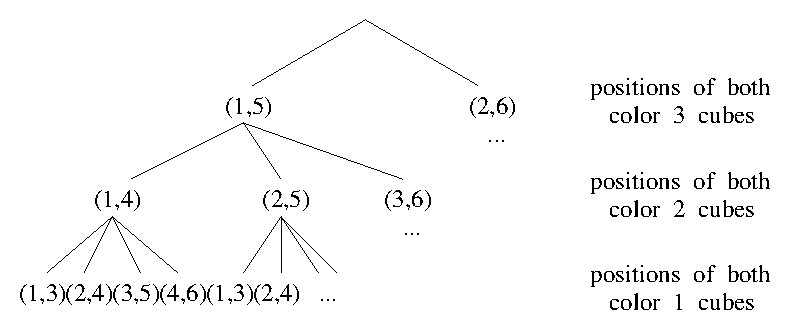
\includegraphics[scale=.65]{\locpath/figures/langford/arbre_en}
%\end{figure}
\begin{figure}[t!]
\centering
\resizebox {\columnwidth} {!} {
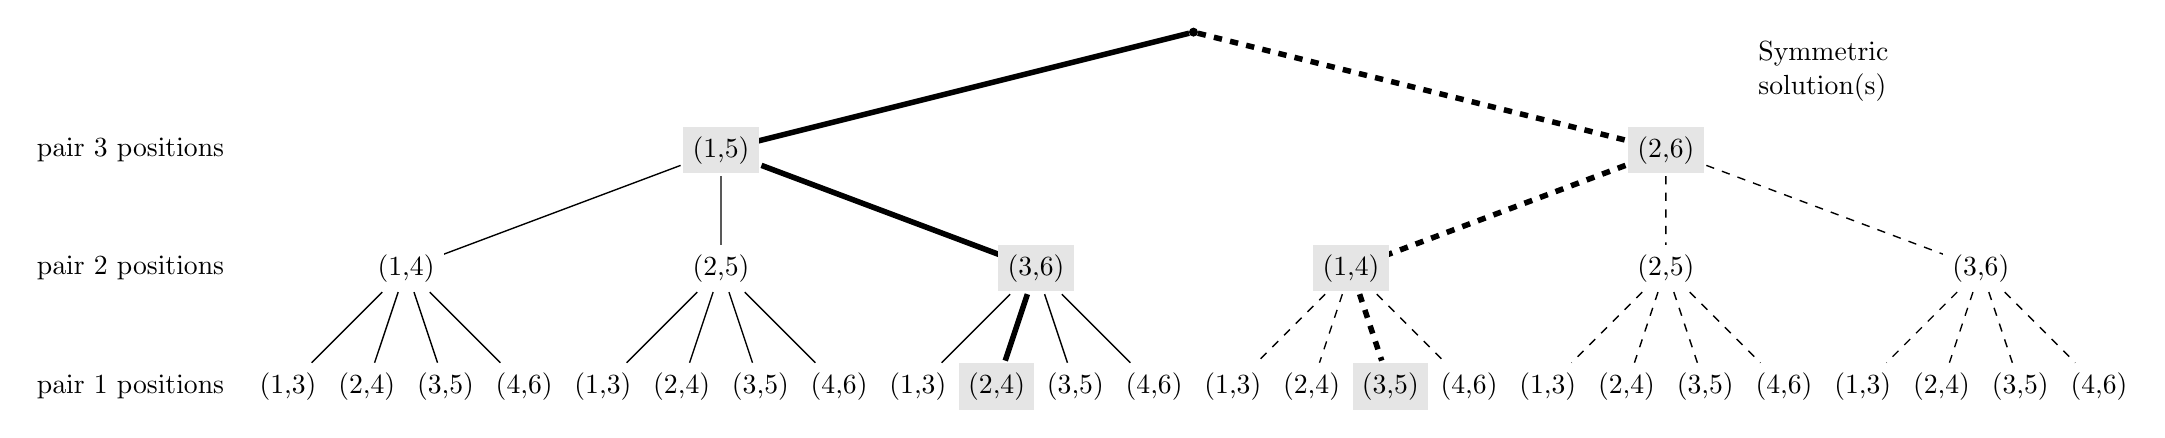
\begin{tikzpicture}[sibling distance=12cm]
\node at (-13.5,-1.5) {pair 3 positions};
\node at (-13.5,-3) {pair 2 positions};
\node at (-13.5,-4.5) {pair 1 positions};
\node [align=left] at (8,-.5) {Symmetric\\solution(s)};
\node  [circle,draw,fill,inner sep=1] {}
  child [line width=2pt] { [sibling distance=4cm] node [fill=black!10] {(1,5)}
    child [line width=.5pt] { [sibling distance=10mm] node [fill=white] {(1,4)}
      child {node {(1,3)}}
      child {node {(2,4)}}
      child {node {(3,5)}}
      child {node {(4,6)}}
    }
    child [line width=.5pt] { [sibling distance=10mm] node [fill=white] {(2,5)}
      child {node {(1,3)}}
      child {node {(2,4)}}
      child {node {(3,5)}}
      child {node {(4,6)}}
    }
    child { [sibling distance=10mm] node [fill=black!10] {(3,6)}
      child [line width=.5pt] {node {(1,3)}}
      child {node [fill=black!10] {(2,4)}}
      child [line width=.5pt] {node {(3,5)}}
      child [line width=.5pt] {node {(4,6)}}
    }
  }
  child [dashed,line width=2pt] { [sibling distance=4cm] node [fill=black!10] {(2,6)}
    child { [sibling distance=10mm] node [fill=black!10] {(1,4)}
      child [line width=.5pt] {node {(1,3)}}
      child [line width=.5pt] {node {(2,4)}}
      child {node [fill=black!10] {(3,5)}}
      child [line width=.5pt] {node {(4,6)}}
    }
    child [line width=.5pt] { [sibling distance=10mm] node [fill=white] {(2,5)}
      child {node {(1,3)}}
      child {node {(2,4)}}
      child {node {(3,5)}}
      child {node {(4,6)}}
    }
    child [line width=.5pt] { [sibling distance=10mm] node [fill=white] {(3,6)}
      child {node {(1,3)}}
      child {node {(2,4)}}
      child {node {(3,5)}}
      child {node {(4,6)}}
    }
  }
;
\end{tikzpicture}
}
\caption{Search tree for $L(2,3)$}
\label{fig:arbre}
\end{figure}
In order to solve $L(2,n)$, we consider a tree of height $n$: see example of $L(2,3)$ in figure~\ref{fig:arbre}.

\begin{itemize}   
\item[-] Every level of the tree corresponds to a color.
\item[-] Each node of the tree corresponds to the placement of a pair of cubes without worrying about the other colors. Color $p$ is represented at depth $n-p+1$, where the first node corresponds to the first possible placement (positions 1 and $p+2$) and $i^{th}$ node corresponds to the placement of the first cube of color $p$ in position $i, \ i \in [1, \ 2n-1-p]$.
\item[-] Solutions are leaves generated without any placement conflict.
\item[-] As we consider the solution up to a symmetry, the left part is represented dashed and is in fact not traversed.
\end{itemize}

There are many ways to browse the tree and find the solutions: \emph{backtracking}, \emph{forward-checking}, \emph{backjumping}, etc \cite{prosser93hybrid}. 
We limit our study to the naive \emph{backtrack} resolution and choose to evaluate the variables and their values in a static order; in a depth-first manner, the solutions are built incrementally and if a partial assignment can be aborted, the branch is cut. A solution is found each time a leaf is reached.
% presents a backtrack search with the previous CSP representation.

The recommendation for performance on GPU accelerators is to use non test-based programs.
Due to its irregularity, the basic \emph{backtracking} algorithm, presented on figure~\ref{backtrack}, is not supposed to suit the GPU architecture.
Thus a vectorized version is given when evaluating the assignments at the leaves' level, with one of the two following ways: assignments can be prepared on each tree node or totally set on final leaves before testing the satisfiability of the built solution (figure~\ref{regularized}).

\begin{figure}[t!]
\begin{minipage}[b]{0.45\linewidth}
\footnotesize
\begin{verbatim}
while not done do
 test pair            <- test
 if successful then 
   if max depth then
     count solution
     higher pair	                  
   else
     lower pair       <- remove
 else
   higher pair        <- add
\end{verbatim}
\caption{Backtrack algorithm}\label{backtrack}
\end{minipage}
\begin{minipage}[b]{0.45\linewidth}
\footnotesize
\begin{verbatim}
for pair 1 positions
  assignment                   <- add
  for pair 2 positions
    assignment                 <- add
    for ...
      for pair n positions
        assignment             <- add
        if final test ok then  
          count solution
\end{verbatim}
\caption{Regularized algorithm}\label{regularized}
\end{minipage}
\end{figure}

\subsubsection{Data representation}

\begin{figure}[t!]
\begin{minipage}[b]{0.40\linewidth}
\centering
\includegraphics[width=\columnwidth]{\locpath/figures/langford/positions_lgf}
\caption{ Bitwise representation of pairs positions in $L(2,3)$} \label{fig:comb1}
\end{minipage}
\hfill
\begin{minipage}[b]{0.55\linewidth}
\centering
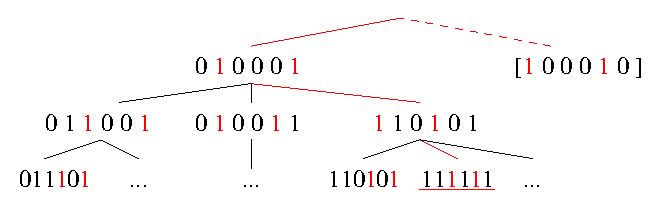
\includegraphics[width=\columnwidth]{\locpath/figures/langford/pos_lgf_v2}
\caption{Bitwise representation of the Langford $L(2,3)$ placement tree}\label{fig:pos_lgf}
\end{minipage}
\end{figure}

In order to count every Langford problem solution, we first identify all possible combinations for one color without worrying about the other ones. 
Each possible combination is coded within an integer, one bit to 1 corresponding to a cube presence, a 0 to its absence. This is what we called a \emph{mask}.
This way figure~\ref{fig:comb1} presents the possible combinations to place the one, two and three weight cubes for the $L(2,3)$ Langford instance.

Furthermore the masks can be used to evaluate the partial placements of a chosen set of colors: all the 1 correspond to occupied positions; the assignment is consistent \emph{iff} there are as many 1 as the number of cubes set for the assignment. 

With the aim to find solutions, we just have to go all over the tree and \emph{sum} one combination of each of the colors: a solution is found \emph{iff} all the bits of the sum are set to 1. 

Each route on the tree can be evaluated individually and independently; then it can be evaluated as a thread on the GPU.
This way the problem is massively parallel and can be, indeed, computed on GPU. figure~\ref{fig:pos_lgf} represents the tree masks' representation.

\subsubsection{Specific operations and algorithms}

Three main operations are required in order to perform the tree search. 
%The first one, allowing to check if a pair can be added to a given partial assignment, is only necessary for the original backtrack scheme.
%The second one, used for both backtrack and regularized methods, aims to add a pair to a given assignment. 
The first one, used for both backtrack and regularized methods, aims to add a pair to a given assignment. 
The second one, allowing to check if a pair can be added to a given partial assignment, is only necessary for the original backtrack scheme.
The last one is used for testing if a global assignment is an available solution: it is involved in the regularized version of the Miller algorithm.

\begin{figure}[t!]
\begin{minipage}[b]{0.5\linewidth}
\centering
\includegraphics[scale=.5]{\locpath/figures/langford/test_gen}
\caption{Testing and adding position} \label{fig:test_et}
\end{minipage}
\begin{minipage}[b]{0.5\linewidth}
\centering 
\includegraphics[scale=.75]{\locpath/figures/langford/graphe_repartition}   
\caption{Server client distribution} \label{fig:parallel} 
\end{minipage}
\end{figure}

\paragraph{Add a pair: }
Top of figure~\ref{fig:test_et} presents the way to add a pair to a given assignment.
With a \emph{binary OR}, the new mask contains the combination of the original mask and of the added pair.
This operation can be performed even if the position is not available for the pair (however the resulting mask is inconsistent). 

\paragraph{Test a pair position: }
On the bottom part of the same figure, we test the positioning of a pair on a given mask. 
For this, it is necessary to perform a \emph{binary AND} between the mask and the pair.
\begin{itemize}
	\item[] $=0$: \emph{success}, the pair can be placed here
	\item[] $\neq0$: \emph{error}, try another position
\end{itemize}

\paragraph{Final validity test: }
The last operation is for \emph{a posteriori} checking. For example the mask $101111$, corresponding to a leaf of the tree, is inconsistent and should not be counted among the solutions.
The final placement mask corresponds to a solution \emph{iff} all the places are occupied, which can be tested as $\neg mask = 0$. % \rightarrow solution$ else $inconsistent$.
%We performed a \emph{binary not} on the mask. If there is a zero, so the mask is inconsistent, result will be different of zero. If the mask is full of $1$, result is zero, so we can add one to the number of solutions.
\\

Using this data representation, 
we implemented both \emph{backtrack} and \emph{regularized} versions of the Miller algorithm, as presented in figure~\ref{backtrack} and \ref{regularized}.
% C'est là que je veux changer la structure ....
%: the original backtrack for CPU computation and the regularized one for GPUs.
%As we have seen above, the regularized algorithm is unsuitable due to combinatorial explosion, that is why we use the hybrid method on a distributed architecture.
\\
The next section presents the way we hybridize these two schemes in order to get an efficient parallel implementation of the Miller algorithm.

%%%%%%%%%%%%%%%%%%%%%%%%%%%%%%%%%%%%%%%%
\subsection{Hybrid parallel implementation}
\label{section:parallel_backtrack}
This part presents our methodology to implement Miller's method on a multiGPU cluster.

\paragraph{Tasks generation: }
In order to parallelize the resolution we have to generate tasks. 
Considering the tree representation, we construct tasks by fixing the different values of a first set of variables [pairs] up to a given level. Choosing the development level allows to generate as many tasks as necessary. This leads to a \textit{Finite number of Irregular and Independent Tasks} (\emph{FIIT} applications \cite{krajecki1999object}). 

\paragraph{Cluster parallelization: } 
The generated tasks are independent and we spread them in a client-server manner: a server generates them and makes them available for clients. As we consider the cluster as a set of CPU-GPU(s) machines, the clients are these machines. 
At the machines level, the role of the CPU is, first, to generate work for the GPU(s): it has to generate sub-tasks, by continuing the tree development as if it were a second-level server, and the GPU(s) can be considered as second-level client(s). \\
The sub-tasks generation, at the CPU level, can be made in parallel by the CPU cores. Depending on the GPUs number and their computation power the sub-tasks generation rhythm may be adapted, to maintain a regular workload both for the CPU cores and GPU threads: some CPU cores, not involved in the sub-tasks generation, could be made available for sub-tasks computing.\\
This leads to the 3-level parallelism scheme presented in figure~\ref{fig:parallel}, where $p$, $q$ and $r$ respectively correspond to: ($p$) the server-level tasks generation depth, ($q$) the client-level sub-tasks generation one, ($r$) the remaining depth in the tree evaluation, \textit{i.e.} the number of remaining variables to be set before reaching the leaves.  

\paragraph{\emph{Backtrack} and \emph{regularized} methods hybridization: } 
The Backtrack version of the Miller algorithm suits CPU execution and allows to cut branches during the tree evaluation, reducing the search space and limiting the combinatorial explosion effects. A regularized version had to be developed, since GPUs execution requires synchronous execution of the threads, with as few branching divergence as possible; however this method imposes to browse the entire search space and is too time-consuming. \\
We propose to hybridize the two methods in order to take advantage of both of them for the multiGPU parallel execution: 
for tasks and sub-tasks generated at sever and client levels, the tree development by the CPU cores is made using the backtrack method, cutting branches as soon as possible [and generating only possible tasks]; when computing the sub-tasks generated at client-level, the CPU cores involved in the sub-tasks resolution use the backtrack method and the GPU threads the regularized one. 

%With this method it is necessary to browse the entire tree but this requires using all the search space and it is too time-consuming.

%In order to overcome this we divide the work between CPU and GPU. The CPU generates some levels of the tree and creates tasks. Then GPU and CPU cores divide up the workload in order to achieve the generation on the latest levels of the tree. 
%With this method, inconsistent branches can be cut on highest level and GPU/CPU cores only compute possibly consistent tasks.

%This representation enables a server-client model to distribute the tasks: the server generates independent sub-problems at a chosen depth in the tree, treated by clients. 
%Each client decomposes the sub-problem into tasks, distributed over the GPU/CPU cores, Fig.~\ref{fig:parallel}.

%By doing so numerous branches have been cut from the main tree during generation stage and GPU/CPU tasks are faster due to their lower depth. Despite the combinatorial explosion of this kind of problem, we can consider solve it in a massively parallel manner on multiGPU clusters.
 
%The tree representation allows to generate tasks at a chosen level, which leads to a \textit{Finite number of Irregular and Independent Tasks} (\emph{FIIT} applications \cite{krajecki1999object}).
%We set up a server-client distribution. The server, client and GPU parts have their own development depth, respectively $p$, $q$ and $r$, $p+q+r=n$, Fig.~\ref{fig:parallel}.
%\begin{itemize}
%\item \texttt{Server} generates sub-problems by placing $p$ pairs on masks with the $backtrack$ algorithm.
%\item \texttt{Client} starts with a mask generated by the server and produces tasks by adding $q$ pairs in the initial mask, with the $backtrack$ algorithm. Then the client creates specific tasks by pre-computing the available positions for placing pairs. For example with the $10100110$ mask the second pair can be placed on only two positions, $01001000$ and $00001001$, that match positions 2-5 and 5-8. Instead of browsing all the 5 positions and test, the GPU just has to try 2 positions for this pair. Thus we greatly reduce the GPU load computation.
%\item \texttt{CPUs and GPUs} can compute in competition. Whereas CPUs use standard backtrack, GPUs generate leaves using the regularized method and adding successive pairs on their masks without any test.  
%\end{itemize}

\subsection{Experiments tuning}

In order to take advantage of all the computing power of the GPU we have to refine the way we use them: this section presents the experimental study required to choose optimal settings. This tuning allowed us to prove our proposal on significant instances of the Langford problem.

\paragraph{Registers, blocks and grid: }

In order to use all GPUs capabilities, the first way was to fill the blocks and grid. To maximize occupancy (ratio between active warps and the total number of warps) NVIDIA suggests to use 1024 threads per block to improve GPU performances and proposes a CUDA occupancy calculator\footnote{\url{http://developer.download.nvidia.com/compute/cuda/CUDA_Occupancy_calculator.xls}}. But, confirmed by the Volkov's results\cite{Volkov}, we experimented that better performances may be obtained using lower occupancy. Indeed, another critical criterion is the inner GPU registers occupation. 
The optimal number of registers ($57$ registers) is obtained by setting 9 pairs placed on the client for $L(2,15)$, thus 6 pairs are remaining for GPU computation.

\begin{figure}[t!]
\centering
\includegraphics[scale=.4]{\locpath/figures/langford/graphe_15_9}
\caption{Time depending on grid and block size on $n=15$}
\label{f7}
\end{figure}

In order to tune the blocks and grid sizes, we performed tests on the ROMEO architecture. 
%0 With this value we obtained an optimized number of registers by thread . 
Figure~\ref{f7} represents the time in relation with the number of blocks per grid and the number of threads per block. 
The most relevant result, observed as a local minimum on the 3D surface, is obtained near 64 or 96 threads per block; for the grid size, the limitation is relative to the GPU global memory size.
It can be noted that we do not need shared memory because their are no data exchanges between threads. 
This allows us to use the total available memory for the L1 cache for each thread.

\paragraph{Streams:}
A client has to prepare work for GPU. There are four main steps: generate the tasks, load them into the device memory, process the task on the GPU and then get the results.

\begin{figure}[t!]
\begin{minipage}[b]{0.48\linewidth}
\centering
\includegraphics[width=\columnwidth]{\locpath/figures/langford/streams.jpeg}
\caption{Computing time depending on streams number}
\label{fig:streams}
\end{minipage}
\hfill
\begin{minipage}[b]{0.48\linewidth}
\centering
\includegraphics[width=\columnwidth]{\locpath/figures/langford/graphe_cores.pdf}
\caption{CPU cores optimal distribution for GPU feeding}\label{cores_rep}
\end{minipage}
\end{figure}

CPU-GPU memory transfers cause huge time penalties (about 400 cycles latency for transfers between CPU memory and GPU \emph{device memory}). 
At first, we had no overlapping between memory transfer and kernel computation because the tasks generation on CPU was too long compared to the kernel computation.
To reduce the tasks generation time we used OpenMP in order to use the eight available CPU cores.
Thus CPU computation was totally hidden by memory transfers and GPU kernel computation. We tried using up to 7 streams; as shown by figure~\ref{fig:streams}, using only two simultaneous streams did not improve efficiency because the four steps did not overlap completely; the best performances were obtained with three streams; the slow increase in the next values is caused by synchronization overhead and CUDA streams management.

\paragraph{Setting up the server, client and GPU depths: }
We now have to set the depths of each actor, server $(p)$, client $(q)$ and GPU $(r)$ (see figure~\ref{fig:parallel}).

First we set the $r = 5$ for large instances because of the GPU limitation in terms of registers by threads, exacerbated by the use of numerous $64bits$ integers. For $r \geq 6$, we get too many registers (64) and for $r \leq 4$ the GPU computation is too fast compared to the memory load overhead.

Clients are the buffers between the server and the GPUs: 
$q = n - p- r$.
So we have conducted tests by varying the server depth, $p$. The best result is obtained for $p=3$ and performance decreases quickly for higher values. This can be explained since more levels on the server generates smaller tasks; thus GPU use is not long enough to overlap memory exchanges.
% because with more levels on the server, tasks are smaller and then the GPU work is not long enough in view of memory exchanges.

\paragraph{CPU: Feed the GPUs and compute}
The first work of CPU cores is to prepare tasks for GPU so that we can generate overlapping between memory load and kernel computation. 
In this configuration using eight cores to generate GPU tasks under-uses CPU computation power. 
It is the reason why we propose to use some of the CPU cores to take part of the sub-problems treatment. 
Figure~\ref{cores_rep} represents computation time in relation with different task distributions between CPU and GPU.
We experimentally demonstrated that only 4 or 5 CPU cores are enough to feed GPU, the other ones can be used to perform backtrack resolution in competition with GPUs.

\subsection{Results}

\paragraph{Regularized method results}
We now show the results obtained for our massively parallel scheme using the previous optimizations, comparing the computation times of successive instances of the Langford problem. 
These tests were performed on 20 nodes of the ROMEO supercomputer, hence 40 CPU/GPU machines.

The previous limit with Miller's algorithm was $L(2,19)$, obtained in 1999 after 2.5 years of sequential effort and at the same time after 2 months with a distributed approach\cite{Mil00}. 
Our computation scheme allowed us to obtain it in less than 4 hours (Table \ref{tab:result_base_regu}), this being not only due to Moore law progress.\\
Note that the computation is 1.6 faster with CPU+GPU together than using 8 CPU cores. 
In addition, the GPUs compute $200000\times$ more nodes of the search tree than the CPUs, with a faster time.

\begin{table}[t!]
\begin{subfigure}[b]{0.5\linewidth}
\centering
\begin{tabular}{l r r r}
					\hline
					$n$ & CPU (8c) &  GPU (4c) +  &  \hspace*{-.8em}CPU (4c) \\
					\hline
					\hline
					15	& 2.5 & 1.5 & \\
					16  & 21.2 &14.3 & \\
					17  & 200.3 &120.5 &\\
					18  & 1971.0 &1178.2 &\\
					19  & 22594.2 & 13960.8 & \\ 
					\hline
\end{tabular}
\caption{Regularized method (seconds)}
\label{tab:result_base_regu}
\end{subfigure}
\begin{subfigure}[b]{0.5\linewidth}
\centering
\begin{tabular}{ l r r r }
					\hline
					$n$ & CPU (8c) &  GPU (4c) +  &  \hspace*{-.8em}CPU (4c) \\
					\hline
					\hline
					17  & 29.8 & 7.3&\\
					18  & 290.0 & 73.6&\\
					19  & 3197.5 & 803.5& \\
					20  & -- & 9436.9 &\\
					21  & -- & 118512.4& \\ 
					\hline
\end{tabular}	
\caption{Backtrack  (seconds)}
\label{tab:result_backtrack}
\end{subfigure}
\caption{Comparison between multi-core processors and GPUs for regularized and backtrack method}
\end{table}

The computation time between two different consecutive instances being multiplied by $10$ approximately, this could allow us to obtain $L(2,20)$ in a reasonable time.


\paragraph{Backtracking on GPUs}

It appears at first sight that using backtracking on GPUs without any regularization is a bad idea due to threads synchronization issues.
But in order to compare CPU and GPU computation power in the same conditions we decide to implement the original backtrack method on GPU (see figure~\ref{backtrack}) with only minor modifications.
In these conditions we observe very efficient work of the NVIDIA scheduler, which perfectly handles threads de-synchronization.
Thus we use the same server-client distribution as in \ref{section:parallel_backtrack}, each client generates masks for both CPU and GPU cores. 
The workload is then statically distributed on GPU and CPU cores.
Executing the backtrack algorithm on a randomly chosen set of sub-problems allowed us to set the GPU/CPU distribution ratio experimentally to 80/20\%.

The experiments were performed on 129 nodes of the ROMEO supercomputer, hence 258 CPU/GPU machines and one node for the server. 
Table \ref{tab:result_backtrack} shows the results with this configuration. 
This method first allowed us to perform the computation of $L(2,19)$ in less than 15 minutes, $15\times$ faster than with the regularized method; then, we pushed the limitations of the Miller algorithm up to $L(2,20)$ in less than 3 hours and even $L(2,21)$ in about $33$ hours\footnote{Even if this instance has no interest since it is known to have no solution}.

This exhibits the ability of the GPU scheduler to manage highly irregular tasks. 
It proves that GPUs are adapted even to solve combinatorial problems, which they were not supposed to be.

\section{Godfrey's algebraic method}
The previous part presents the Miller algorithm for the Langford problem, this method cannot achieve bigger instances than the $L(2,21)$.\\
An algebraic representation of the Langford problem has been proposed by M. Godfrey in 2002.
In order to break the limitation of $L(2,24)$ we already used this very efficient problem specific method.
In this part we describe this algorithm and optimizations, and then our implementation on multiGPU clusters.
\subsection{Method description}
Consider $L(2,3)$ and $X=(X_1,X_2,X_3,X_4,X_5,X_6)$. 
It proposes to modelize $L(2,3)$ by: 
\begin{equation}
\begin{aligned}
F(X,3) = & (X_1X_3+X_2X_4+X_3X_5+X_4X_6)\times \\
& (X_1X_4+X_2X_5+X_3X_6)\times\\
& (X_1X_5+X_2X_6)
\end{aligned}
\end{equation}
In this approach each term represents a position of both cubes of a given color and a solution to the problem corresponds to a term developed as $(X_1X_2X_3X_4X_5X_6)$; thus the number of solutions is equal to the coefficient of this monomial in the development. 
More generally, the solutions to $L(2,n)$ can be deduced from $(X_1X_2X_3X_4X_5...X_{2n})$ terms in the development of $F(X,n)$.

If \ \ $G(X,n) = X_1 ... X_{2n} F(X,n)$ then it has been shown that: 

\begin{equation}
\sum\limits_{(x_1,...,x_{2n}) \in \{-1,1\}^{2n}} G(X,n)_{(x_1,...,x_{2n})} =  2^{2n+1}L(2,n)
\end{equation}

So \hspace*{2cm}
\begin{equation}
\sum\limits_{(x_1,...,x_{2n}) \in \{-1,1\}^{2n}} \big( \prod\limits_{i=1}^{2n} x_i \big) \prod\limits_{i=1}^{n} \sum\limits_{k=1}^{2n-i-1} x_kx_{k+i+1} = 2^{2n+1} L(2,n)
\end{equation}

\noindent That allows to get $L(2,n)$ from polynomial evaluations.
The computational complexity of $L(2,n)$ is of $O(4^n\times n^2)$ and an efficient big integer arithmetic is necessary. 
This principle can be optimized by taking into account the symmetries of the problem and using the Gray code: these optimizations are described below.

\subsection{Optimizations}
Some works focused on finding optimizations for this arithmetic method\cite{CReSTIC-1154}. 
Here we explain the symmetric and computation optimizations used in our algorithm.

\subsubsection{Evaluation parity: }
As $[F(-X,n) = F(X,n)]$, $G$ is not affected by a global sign change. 
In the same way the global sign does not change if we change the sign of each pair or impair variable.

Using these optimizations we can set the value of two variables and accordingly divide the computation time and result size by four.

\subsubsection{Symmetry summing: }
In this problem we have to count each solution up to a symmetry; thus for the first pair of cubes we can stop the computation at half of the available positions considering 

\noindent $S'_1(x) = \sum_{k=1}^{n-1}x_kx_{k+2}$ instead of $S_1(x) = \sum_{k=1}^{2n-2} x_kx_{k+2}$.
The result is divided by 2. 

\subsubsection{Sums order: }
Each evaluation of $ S_i(x) = \sum_{k=1}^{2n-i-1} x_kx_{k+i+1} $, before multiplying might be very important regarding to the computation time for this sum. 
Changing only one value of $ x_i $ at a time, we can recompute the sum using the previous one without global re-computation. 
Indeed, we order the evaluations of the outer sum using Gray code sequence. 
Then the computation time is considerably reduced.  

Based on all these improvements and optimizations we can use the Godfrey method in order to solve huge instances of the Langford problem. 
The next section develops the main issues of our multiGPU architecture implementation. 

\subsection{Implementation details}
In this part we present the specific adaptations required to implement the Godfrey method on a multiGPU architecture.

\subsubsection{Optimized big integer arithmetic: }

In each step of computation, the value of each $S_i$ can reach $2n-i-1$ in absolute value, and their product can reach $\frac{(2n-2)!}{(n-2)!}$. 
As we have to sum the $S_i$ product on $2^{2n}$ values, in the worst case we have to store a value up to $2^{2n}\frac{(2n-2)!}{(n-2)!}$, which corresponds to $10^{61}$ for $n=28$, with about 200 bits.

So we need few big integer arithmetic functions. After testing existing libraries like GMP for CPU or CUMP for GPU, we came to the conclusion that they implement a huge number of functionalities and are not really optimized for our specific problem implementation: product of "small" values and sum of "huge" values. 

Finally, we developed a light CPU and GPU library adapted to our needs.
In the sum for example, as maintaining carries has an important time penalty, we have chosen to delay the spread of carries by using buffers: carries are accumulated and spread only when useful (for example when the buffer is full).
Figure~\ref{fig:big-integer} represents this big integer handling.
\begin{figure}[htbp]
\centering
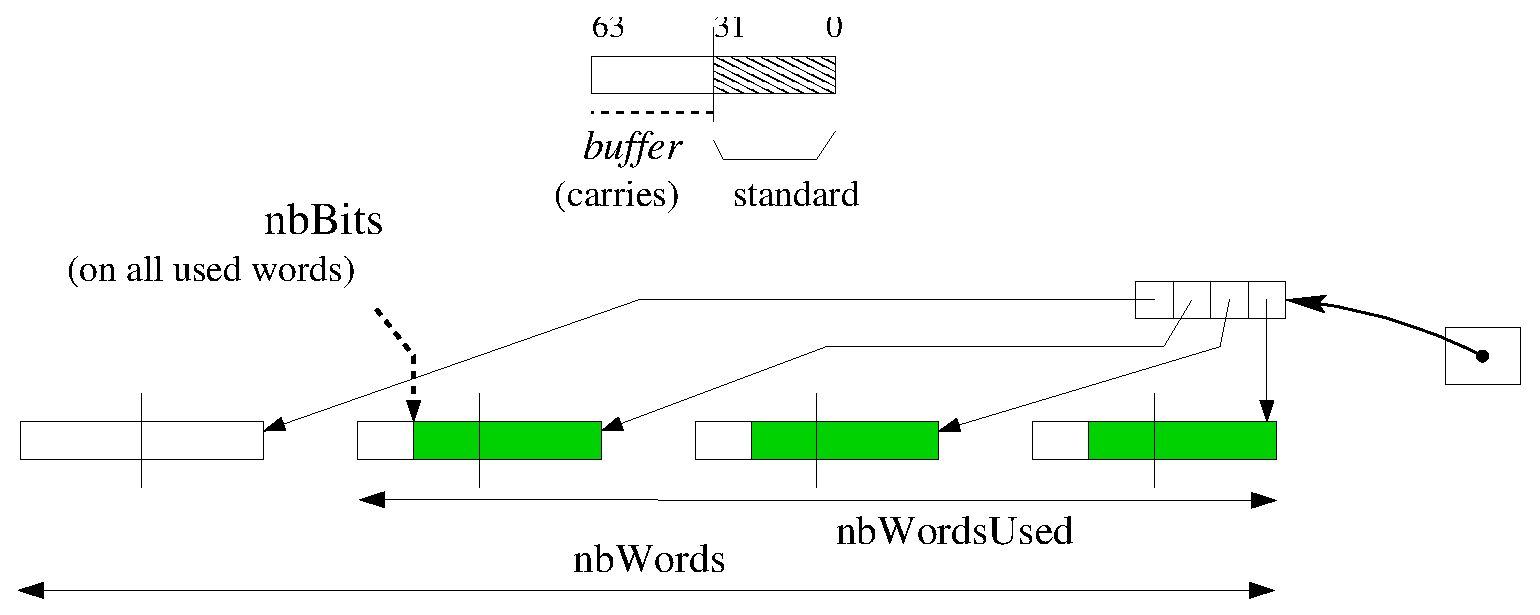
\includegraphics[scale=.5]{\locpath/figures/langford/lgf_grands_entiers}
\caption{Big integer representation, 64 bits words}
\label{fig:big-integer}
\end{figure}


\subsubsection{Gray sequence in memory: }
The Gray sequence cannot be stored in an array because it would be too large (it would contain $2^{2n}$ byte values). This is the reason why only one part of the Gray code sequence is stored in memory and the missing terms are directly computed from the known ones using arithmetic considerations.
The size of the stored part of the Gray code sequence is chosen to be as large as possible to be contained in the processor's cache memory, the L1 cache for the GPUs threads: so the accesses are fastened and the computation of the Gray code is optimized.
For an efficient use of the E5-2650 v2 ROMEO's CPUs, which disposes of 20 MB of level-3 cache, the CPU Gray code sequence is developed recursively up to depth 25. For the K20Xm ROMEO's GPUs, which dispose of 8 KB of constant memory, the sequence is developed up to depth 15. The rest of the memory is used for the computation itself. 
%As the Gray sequence is not entirely stored in memory, 
%As we show, all the gray sequence is not in memory, in order to compute the next value when the array is exceeded a modulus method is used for recompute the next value.

\subsubsection{Tasks generation and computation: }
\label{sec:tasks}

In order to perform the computation of the polynomial, two variables can be set among the $2n$ available. For the tasks generation we choose a number $p$ of variables to generate $2^p$ tasks by developing the evaluation tree to depth $p$.\\
 
 
The tasks are spread over the cluster, either synchronously or asynchronously.

\paragraph{Synchronous computation: }
A first experiment was carried out with an MPI distribution of the tasks of the previous model. 
Each MPI process finds its tasks list based on its process \textit{id}; then converting each task number into binary gives the task's initialization. 
The processes work independently; finally the root process ($id=0$) gathers all the computed numbers of solutions and sums them.

\paragraph{Asynchronous computation: }
\label{section:asynchronous}
In this case the tasks can be computed independently. 
As with the synchronous computation, the tasks' initializations are retrieved from their number. 
Each machine can get a task,  compute it, and then store its result; then when all the tasks have been computed, the partial sums are added together and the total result is provided. 

%In this case if a task is cancel due to machine error or another problem, it can be restart without compromising the end of execution.

%\subsubsection{Efficient computation}
%The computation of any task can be summarized in the four following steps:
%\begin{itemize}
%\item First it is necessary to initialize the task: with depth level $p$, $X_1=X_2=1$ and the next $p$ variables are assigned to $1$ or $-1$ depending on the task's id. The following ones are set to $1$ for example.
%\item Secondly it is necessary to set the value of each $S_i$ with the sum of $X_kX_{k + i + 1}$.
%\item Then CPU and GPU, concurrently working, go through all of the Gray sequence on the remaining $2n-p-2$ variables, by updating the $S_i$ and sum their product at each step.
%\item Finally the CPU cores computed results are summed over a shared variable; the GPU sub-tasks results are copied back and then summed with the global result.
%\end{itemize}

\subsection{Experimental settings}
This part presents the experimental context and methodology, and the way the experiments were carried out.
This study has similar goals as for the Miller's resolution experiments.

\subsubsection{Experimental methodology: }
We present here the way the experimental settings were chosen.
Firstly we define the tasks distribution, secondly we set the number of threads per GPU block; finally, we set the CPU/GPU distribution.

\paragraph{Tasks distribution depth: }
This value being set it is important to get a high number of blocks to maintain sufficient GPU load.
Thus we have to determine the best number of tasks for the distribution. As presented in part \ref{sec:tasks} the number $p$ of bits determines $2^p$ tasks. On the one hand, too many tasks are a limitation for the GPU that cannot store all the tasks in its 6GB memory. On the other hand, not enough tasks means longer tasks and too few blocks to fill the GPU grid. figure~\ref{fig:graphe_prof} shows that for the $L(2,23)$ instance the best task number is with generation depth 28.

\paragraph{Number of threads per block: }
In order to take advantage of the GPU computation power, we have to determine the threads/block distribution. Inspired by our experiments with Miller's algorithm we know that the best value may appear at lower occupancy. We perform tests on a given tasks set varying the threads/block number and grid size associated. 
Figure~\ref{fig:graphe_threads} presents the tests performed on the $n=20$ problem: the best distribution is around $128$ threads per block. 
\begin{figure}[t!]
\centering 
\includegraphics[scale=.55]{\locpath/figures/langford/graphe_threads}
\caption{$L(2,20)$, number of threads per block}
\label{fig:graphe_threads}
\end{figure}

\begin{figure}[t!]
\begin{subfigure}[b]{0.5\linewidth}
\centering 
\includegraphics[scale=.5]{\locpath/figures/langford/graphe_prof}
\caption{Influence on server generation depth}
\label{fig:graphe_prof}
\end{subfigure}
\begin{subfigure}[b]{0.5\linewidth}
\centering
\includegraphics[scale=.5]{\locpath/figures/langford/graphe_cpu_gpu}
\caption{Influence of tasks repartition}
\label{fig:graphe_rep}
\end{subfigure}
\caption{Influences of repartitions of depths and CPU-GPU tasks}
\end{figure}

\subsubsection{CPU vs GPU distribution: }
The GPU and CPU computation algorithm will approximately be the same. 
In order to take advantage of all the computational power of both components we have to balance tasks between CPU and GPU. 
We performed tests by changing the CPU/GPU distribution based on simulations on a chosen set of tasks.  
Figure~\ref{fig:graphe_rep} shows that the best distribution is obtained when the GPU handles 65\% of the tasks. 
This optimal load repartition directly results from the intrinsics computational power of each component; this repartition should be adapted if using a more powerful GPU like Tesla K40 or K80.

\subsubsection{Computing context: }

As presented in part~\ref{sec:part1_ROMEO}, we used the ROMEO supercomputer to perform our tests and computations.
%We use the same supercomputer to perform that computation that we use for the Miller method (section \ref{sec:context}), the ROMEO cluster which use Slurm as node reservation software.
On this supercomputer SLURM\cite{slurm} is used as a reservation and job queue manager.
This software allows two reservation modes: a static one-job limited reservation or the opportunity to dynamically submit several jobs in a Best-Effort manner.

\paragraph{Static distribution: }
In this case we used the synchronous distribution presented in \ref{section:asynchronous}. 
We submited a reservation with the number of MPI processes and the number of cores per process.
This method is useful to get the results quickly if we can get at once a large amount of computation resources. It was used to perform the computation of small problems, and even for $L(2,23)$ and $L(2,24)$.\\
As an issue, it has to be noted that it is difficult to quickly obtain a very large reservation on such a shared cluster, since many projects are currently running. 

\paragraph{Best effort: }
SLURM allows to submit tasks in the specific Best-Effort queue, which does not count in the user \textit{fair-share}. In this queue, if a node is free and nobody is using it, the reservation is set for a job in the best effort queue for a minimum time reservation. 
If another user asks for a reservation and requests this node, the best effort job is killed (with, for example, a SIGTERM signal). This method, based on asynchronous computation, enables a maximal use of the computational resources without blocking for a long time the entire cluster.
%This global computation process is fault-tolerant since no result is provided for aborted tasks, that are computed again.

For $L(2,27)$ and even more for $L(2,28)$ the total time required is too important to use the whole machine off a challenge period, thus we chose to compute in a Best-Effort manner.
In order to fit with this submission method we chose a reasonable time-per-task, sufficient to optimize the treatments with low loading overhead, but not too long so that killed tasks are not too penalizing for the global computation time. We empirically chose to run 15-20 minute tasks and thus we considered $p=15$ for $n=27$ and $p=17$ for $n=28$. 

The best effort based algorithm is presented on figure~\ref{fig:graphe_besteffort}.
The task handler maintains a maximum of 256 tasks in the queue; in addition the entire process is designed to be fault-tolerant since killed tasks have to be launched again.
When finished, the tasks generate an output containing the number of solutions and computation time, that is stored as a file or database entry. 
At the end the outputs of the different tasks are merged and the global result can be provided.  

\begin{figure}[t!]
\centering
\includegraphics[scale=.6]{\locpath/figures/langford/best_effort}
\caption{Best-effort distribution}
\label{fig:graphe_besteffort}
\end{figure}

%\begin{algorithm}[htbp]
%\caption{Server distribution}
%\begin{algorithmic} 
%\STATE \textbf{Variables :}
%\STATE $TQ$: tasks queue, task = integer
%\STATE $FQ$: finished tasks queue, task = integer
%\STATE $BEQ$: number of elements in the Best-Effort queue
%\STATE $N$: number of tasks
%\STATE $result$: final result
%\STATE $nbMachines$: Best-Effort queue jobs limitation
%\STATE 
%\STATE \textbf{Begin}
%\STATE $TQ\leftarrow$generate\_tasks($N$)
%\WHILE{$\#FQ \neq N$}
%\IF{$BEQ < nbMachines$}
%\STATE Start($TQ.next$)
%\ENDIF
%\ENDWHILE
%\STATE $result\leftarrow$sum($FQ$)
%\STATE \textbf{End}
%\end{algorithmic}
%\label{algo:server}
%\end{algorithm}
%
%\begin{algorithm}[htbp]
%\caption{Client task handling}
%\begin{algorithmic}
%\STATE \textbf{Variables :}
%\STATE $TQ$: tasks queue, task = integer
%\STATE $FQ$: finished tasks queue, task = integer
%\STATE $n$: number of this task
%\STATE 
%\STATE \textbf{Signal handler :}
%\IF{$SIGKILL$}
%\STATE put $n$ in the $TQ$
%\ENDIF
%\STATE 
%\STATE \textbf{Begin}
%\STATE $solution\leftarrow$compute($N$)
%\IF{$Error$}
%\STATE put $n$ in $TQ$
%\ELSE
%\STATE put $solution$ in $FQ$
%\ENDIF
%\STATE \textbf{End}
%\end{algorithmic}
%\label{algo:client}
%\end{algorithm}

\subsection{Results}
After these optimizations and implementation tuning steps, we conducted tests on the ROMEO supercomputer using best-effort queue to solve $L(2,27)$ and $L(2,28)$. 
We started the experiment after an update of the supercomputer, that implied a cluster shutdown. 
Then the machine was restarted and was about 50\% idle for the duration of our challenge. 
The computation lasted less than 2 days for $L(2,27)$ and 23 days for $L(2,28)$. 
The following describes performances considerations.

\textbf{Computing effort -} 
For $L(2,27)$, the effective computation time of the 32,768 tasks was about 30 million seconds (345.4 days), and 165,000" elapsed time (1.9 days); the average time of the tasks was 911", with a standard deviation of 20\%.
For the $L(2,28)$ 131,072 tasks the total computation time was about 1365 days (117 million seconds), as 23 day elapsed time; the tasks lasted 1321" on average with a 12\% standard deviation.

\textbf{Best-effort overhead -} 
With $L(2,27)$ we used a specific database to maintain information concerning the tasks: 617 tasks were aborted [by regular user jobs] before finishing (1.9\%), with an average computing time of 766" (43\% of the maximum requested time for a task). This consumed 472873", which overhead represents 1.6\% of the effective computing effort.

\textbf{Cluster occupancy -}
Figure~\ref{fig:graphe_15minutes_27} presents the tasks resolution over the two computation days for $L(2,27)$.
The experiment elapse time was 164700" (1.9 days). Compared to the effective computation time, we used an average of 181.2 machines (CPU-GPU couples): this represents 69.7\% of the entire cluster.
 
Figure~\ref{fig:graphe_15minutes_28} presents the tasks resolution flow during the 23 days computation for $L(2,28)$. We used about 99 machines, which represents 38\% of the 230 available nodes.

\begin{figure}[t!]
\begin{subfigure}[b]{0.5\linewidth}
\centering
\includegraphics[scale=.6]{\locpath/figures/langford/graphe_15minutes_petit}
\caption{$L(2,27)$ tasks grouped by 15" slots}
\label{fig:graphe_15minutes_27}
\end{subfigure}
\begin{subfigure}[b]{0.5\linewidth}
\centering
\includegraphics[scale=.6]{\locpath/figures/langford/graphe_15minutes_petit_28}
\caption{$L(2,28)$ tasks grouped by 1 hour slots}
\label{fig:graphe_15minutes_28}
\end{subfigure}
\caption{Task repartition for $L(2,27)$ and $L(2,28)$ }
\end{figure}

For $L(2,27)$, these results confirm that the computation took great advantage of the low occupancy of the cluster during the experiment. 
This allowed us to obtain a weak best-effort overhead, and an important cluster occupancy. 
Unfortunately for $L(2,28)$ on such a long period we got a lower part of the supercomputer dedicated to our computational project.
Thus we are confident in good perspectives for the $L(2,31)$ instance if computed on an even larger cluster or several distributed clusters. 

\section{Conclusion}

This study presents two methods to solve the Langford pairing problem on multi-GPU clusters. 
In its first part the Miller's algorithm is presented. 
Then to break the problem limitations we show optimizations and implementation of Godfrey's algorithm.

\subsection{CSP resolution method}
As any combinatorial problem can be represented as a CSP, the Miller algorithm can be seen as general resolution scheme based on the backtrack tree browsing. 
A three-level tasks generation allows to fit the multiGPU architecture. 
MPI or Best-Effort are used to spread tasks over the cluster, OpenMP for the CPU cores distribution and then CUDA to take advantage of the GPU computation power.
We were able to compute $L(2,20)$ with this regularized method and to get an even better time with the basic backtrack. 
This proves the proposed approach and also exhibits that the GPU scheduler is very efficient at managing highly divergent threads.

\subsection{MultiGPU clusters and best-effort}
In addition and with the aim to beat the Langford limit we present a new implementation of the Godfrey method using GPUs as accelerators. 
In order to use the supercomputer ROMEO, which is shared by a large scientific community, we have implemented a distribution that does not affect the machine load, using a best-effort queue. The computation is fault-tolerant and totally asynchronous.

\paragraph{Langford problem results: }
This study enabled us to compute $L(2,27)$ and $L(2,28)$ in respectively less than 2 days and 23 days on the University of Reims ROMEO supercomputer. 
The total number of solutions is: 

\hspace{3cm} L(2,27) = 111,683,611,098,764,903,232

\hspace{3cm} L(2,28) = 1,607,383,260,609,382,393,152

\paragraph{GPU benefit: }
This study shows the benefit of using GPUs as accelerators for combinatorial problems. 
In Miller's algorithm they handle 80\% of the computation effort and 65\% in Godfrey's.\\
As a near-term prospect, we want to scale and show that it is possible to use the order of 1000 or more GPUs for pure combinatorial problems.\\
The next step of this work is to generalize the method to optimization problems. 
This adds an order of complexity since shared information has to be maintained over a multiGPU cluster. 

We can conclude that even on irregular problems accelerators like GPU can be use and show better results than classical processors. 
 


%%%%%%%%%%%%%%%%%%%%%%%%%%%%%%%%%%%%%%%%%%%%%%%%%%%%%%%%%%%%%%%%%%%%%
%																	%
%	CHAPTER THREE, SOFTWARE AND API									%
%																	%
%%%%%%%%%%%%%%%%%%%%%%%%%%%%%%%%%%%%%%%%%%%%%%%%%%%%%%%%%%%%%%%%%%%%%

\documentclass[11pt,a4paper]{book}
\usepackage[utf8]{inputenc}
\usepackage[english]{babel}
\usepackage{amsmath}
\usepackage{amsfonts}
\usepackage{amssymb}
\usepackage{graphicx}
\usepackage{url}
\usepackage{python}
\usepackage{algpseudocode,algorithm}
\usepackage{tikz}
%\usepackage{todonotes}
\usepackage{makeidx}
\usepackage{enumitem}
\usepackage{array}
\usepackage{makecell}
\usepackage{xcolor}
\usetikzlibrary{positioning}
\usetikzlibrary{decorations.pathreplacing}
\usetikzlibrary{patterns}


\newcommand\todo[1]{\textcolor{red}{#1}}
\newcommand{\locpath}{../..}

\usepackage[left=2.5cm,right=2.5cm,top=2cm,bottom=2.5cm]{geometry}

% Thesis title
%\title{Energy Efficiency, Exascale and Complex Systems}
\title{Vers l'Exascale: Des Probl\`emes Th\'eoriques aux Probl\`emes Appliqu\'es\\
The Way to Exascale: From Theorics to Applied Problems}
% Author
\author{Julien Loiseau}
% Date 
\date{\today}

\makeindex

\begin{document}
\setcounter{chapter}{2}

\documentclass[11pt,a4paper]{book}
\usepackage[utf8]{inputenc}
\usepackage[english]{babel}
\usepackage{amsmath}
\usepackage{amsfonts}
\usepackage{amssymb}
\usepackage{graphicx}
\usepackage{url}
\usepackage{python}
\usepackage{algpseudocode,algorithm}
\usepackage{tikz}
%\usepackage{todonotes}
\usepackage{makeidx}
\usepackage{enumitem}
\usepackage{array}
\usepackage{makecell}
\usepackage{xcolor}
\usetikzlibrary{positioning}
\usetikzlibrary{decorations.pathreplacing}
\usetikzlibrary{patterns}


\newcommand\todo[1]{\textcolor{red}{#1}}
\newcommand{\locpath}{../..}

\usepackage[left=2.5cm,right=2.5cm,top=2cm,bottom=2.5cm]{geometry}

% Thesis title
%\title{Energy Efficiency, Exascale and Complex Systems}
\title{Vers l'Exascale: Des Probl\`emes Th\'eoriques aux Probl\`emes Appliqu\'es\\
The Way to Exascale: From Theorics to Applied Problems}
% Author
\author{Julien Loiseau}
% Date 
\date{\today}

\makeindex

\begin{document}
\setcounter{chapter}{2}

\input{\locpath/chapters/part1/chap3}

\bibliographystyle{alpha}
\bibliography{\locpath/biblio/biblio_langford,\locpath/biblio/biblio_graph,\locpath/biblio/biblio_sph,\locpath/biblio/biblio_hpc}

\end{document}


\bibliographystyle{alpha}
\bibliography{\locpath/biblio/biblio_langford,\locpath/biblio/biblio_graph,\locpath/biblio/biblio_sph,\locpath/biblio/biblio_hpc}

\end{document}


\chapter*{Conclusion}
This part detailed the state of the art theory, hardware and software in High Performance Computing and the tools we need to detail our experiences.

In the first chapter we introduced the models for computation and memory. 
We also detailed the main laws of HPC. 

The second chapter was an overview of hardware architectures in HPC. 
The one that seems to be the most promising regarding computational power and energy consumption seems to be hybrid architectures. 
Supercomputers equipped with classical processors accelerated by devices like GPGPUs, Xeon Phi or, for tomorrow supercomputers, FPGAs. 

In the third section we showed that the tools to target such complex architecture are ready. 
They provide the developer a two or three layer development model with MPI for distribution over processes, OpenMP/PThreads for tasks between the processor's cores and CUDA/OpenCL/OpenMP/OpenACC to target the accelerator. 

We also showed in the last part that the benchmarks proposed to rank those architectures are based on regular computation. 
They are node facing realistic domain scientists code behavior. 
The question that arise is: How the hybrid architecture will handle irregularity in term of computation and communication? 
This question will be developed in the next part through one example for irregular computation and another for irregular communication using accelerators. 




% Chapter Two 
\part{Complex systems}
%\chapter*{Introduction}

%%%%%%%%%%%%%%%%%%%%%%%%%%%%%%%%%%%%%%%%%%%%%%%%%%%%%%%%%%%%%%%%%%%%%
%                                                                   %
% CHAPTER ONE, INTRODUCTION.                                        % 
%                                                                   %
%%%%%%%%%%%%%%%%%%%%%%%%%%%%%%%%%%%%%%%%%%%%%%%%%%%%%%%%%%%%%%%%%%%%%

%%%%%%%%%%%%%%%%%%%%%%%%%%%%%%%%%%%%%%%%%%%%%%%%%%%%%%%%%%%%%%%%%%%%%
%                                                                   %
%	CHAPTER ONE, CHOICES AND SPH                                    %
%                                                                   %
%%%%%%%%%%%%%%%%%%%%%%%%%%%%%%%%%%%%%%%%%%%%%%%%%%%%%%%%%%%%%%%%%%%%%
\chapter{General problem}

\section{Introduction}
In this section we give details on our choices for the generic application confronted to both computation and communication walls on irregular context. 
This problem, Smoothed Particle Hydrodynamics, is described on the physics aspect and the difficulties involved in the resolution on supercomputers.  

\section{Combining irregular behaviors}


\section{Smoothed Particle Hydrodynamics}

\subsection{General description}
Smoothed Particle Hydrodynamics (SPH) is an explicit numerical mesh-free Lagrangian method used to solve hydrodynamical partial differential equations (PDEs) by discretized it into a set of fluid elements called particles. 
This computational method was invented for the purpose of astrophysics simulations by Monaghan, Gingold and Lucy in 1977 \cite{lucy1977numerical,gingold1977smoothed}. 
This first SPH work conserved mass and they later proposed a method which also conserves linear and angular moment \cite{gingold1982kernel}. 
The method was extended for general fluid simulation and many more fields from ballistics to oceanography. 
The development of new reliable, parallel and distributed tools for this method is a challenge for future HPC architectures with the upcoming Exascale systems.

\begin{figure}
\centering
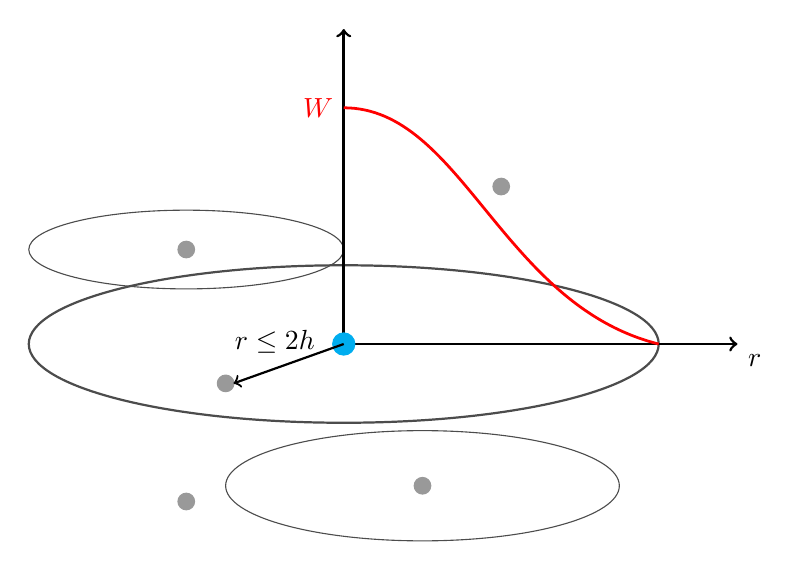
\begin{tikzpicture}
	
	% Others and their ellipse
	\draw [fill,black!40] (.5,1.5) circle (.3em);
	\draw [fill,black!40] (0,0) circle (.3em);
	\draw [fill,black!40] (0,3.2) circle (.3em);
	\draw[black!70] (0,3.2) ellipse (2 and .5);
	\draw [fill,black!40] (3,.2) circle (.3em);
	\draw[black!70] (3,.2) ellipse (2.5 and .7);
	\draw [fill,black!40] (4,4) circle (.3em);
	% Ellipses 
	\draw[line width=.8pt,black!70] (2,2) ellipse (4 and 1);
	% Axes
	\draw[->,line width=1pt] (2,2) -- (7,2) node[anchor=north west] {$r$};
	\draw[->,line width=1pt] (2,2) -- (2,6);
	% bezier for kernel 
	\draw[red,line width=1pt]  (6,2) .. controls (4,2.5) and (3.5,5) .. (2,5) node[red,anchor=east] {$W$};
	% main particle, at the end to cover
	\draw [fill,cyan] (2,2) circle (.4em);
	% Arrows 
	\draw[->,line width=.8pt] (2,2) -- (.6,1.5) node[midway, above,xshift=-.5em] {$r\leq2h$};
\end{tikzpicture}
%\includegraphics[scale=.4]{\locpath/figures/flecsph/sph.pdf}
\caption{SPH kernel $W$ and smoothing length $h$ representation}
\label{fig:sph_base}
\end{figure}

The method, as illustrated in Fig.~\ref{fig:sph_base}, computes the evolution of physical quantities for every particle regarding its neighbors in the radius of its smoothing length $h$. 
The particles in this radius are then valued according to their distance using a smoothing function $W$, also called a kernel. 
The fundamental SPH formulation for any physical quantity $A$ is then to compute with all the neighbors of $b$ of a particle by:
\begin{equation}
A(\vec{r}) \simeq \sum_b \frac{m_b}{\rho_b} A(\vec{r}_b) W ( |\vec{r}-\vec{r}_b|,h)
\end{equation}

On a physics aspect, this method has several advantages:
It can handle deformations, low densities, vacuum, and makes particle tracking easier. 
It also conserves mass, linear and angular momenta, and energy by its construction that implies independence of the numerical resolution. 
Another strong benefit of using SPH is its exact advection of fluid properties. 
Furthermore, the particle structure of SPH easily combines with tree methods for solving Newtonian gravity through N-body simulations.
As a mesh-free method, it avoids the need of grid to calculate the spatial derivatives. 

However, there are cons to consider using SPH: 
It is restricted to low-order rate of convergence on certain PDE formulations; 
It requires careful setup of initial distribution of particles; 
Further, it can be struggle to resolve turbulence-dominated flows and special care must be taken when handling high gradients such as shocks and surface structure of neutron stars.
Many works are leading to handle more cases and to push the limitations of this method \cite{dai2017dual,lind2016incompressible,ren2016dual}.

In this work, we are solving Lagrangian conservation equations (Euler equations) for mass, energy and momentum of an ideal fluid ~\cite{Landau1959}  such that:
\begin{equation}
\frac{d \rho}{d t} = - \rho \nabla \cdot \vec{v}, \quad
\frac{d u}{d t} = \left( \frac{P}{\rho^2} \right) \frac{d \rho}{d t}, \quad
\frac{d \vec{v}}{d t} = - \frac{\nabla P}{\rho}
\end{equation}
with $\rho$ the density, $P$ the pressure, $u$ the internal energy and $v$ the velocity, where $d/dt = \partial_t + \vec{v} \cdot \nabla$ which is convective derivative.

By using the volume element $V_b = m_b / \rho_b$, we can formulate the Newtonian SPH scheme~\cite{rosswog2009} such that
\begin{equation}
\label{eq:rho}
\rho_a = \sum_b m_b W_{ab} (h_a)
\end{equation}
\begin{equation}
\frac{d u_a}{dt} = \frac{P_a}{\rho_a^2} \sum_b m_b \vec{v}_{ab} \cdot \nabla_a W_{ab} 
\end{equation}
\begin{equation}
\frac{d \vec{v}_a}{d t} = - \sum_b m_b \left(\frac{P_a}{\rho_a^2} + \frac{P_b}{\rho_b^2} \right) \nabla_a W_{ab}
\end{equation}
where $W_{ab} = W(| \vec{r}_a - \vec{r}_b |,h)$ is the smoothing kernel. 
The equations we would like to solve allow for emergence of discontinuities from smooth initial data. 
At discontinuities, the entropy increases in shocks. That dissipation occurs inside the shock-front. 
The SPH formulation here is inviscid so we need to handle this dissipation near shocks. 
There are a number of way to handle this problem, but the most widespread approach is to add artificial viscosity (or artificial dissipation) terms in SPH formulation such that:
\begin{equation}
\left(\frac{d u_a}{dt} \right)_{art} = \frac{1}{2} \sum_b m_b \Pi_{ab} \vec{v}_{ab} \cdot \nabla_a W_{ab}
\end{equation}
\begin{equation}
\left(\frac{d\vec{v}_a}{dt} \right)_{art} = - \sum_b m_b \Pi_{ab}\nabla_a W_{ab}
\end{equation}
In general, we can express the equations for internal energy and acceleration with artificial viscosity
\begin{equation}
\label{eq:intern}
\frac{d u_a}{dt} = \sum_b m_b \left(\frac{P_a}{\rho_a^2} + \frac{\Pi_{ab}}{2} \right) \vec{v}_{ab} \cdot \nabla_a W_{ab}
\end{equation}
\begin{equation}
\label{eq:velo}
\frac{d \vec{v}_a}{d t} = - \sum_b m_b \left(\frac{P_a}{\rho_a^2} + \frac{P_b}{\rho_b^2} + \Pi_{ab} \right) \nabla_a W_{ab}
\end{equation}
$\Pi_{ab}$ is the artificial viscosity tensor. 
As long as $\Pi_{ab}$ is symmetric, the conservation of energy, linear and angular momentum is assured by the form of the equation and antisymmetry of the gradient of kernel with respect to the exchange of indices $a$ and $b$. $\Pi_{ab}$ may define different way but here we use~\cite{Monaghan1983} such as: 
\begin{equation}
\Pi_{ab} = \begin{cases}
\frac{- \alpha \bar{c}_{ab} \mu_{ab} + \beta \mu_{ab}^2}{\bar{\rho}_{ab}} & \text{for $\vec{r}_{ab} \cdot \vec{v}_{ab} < 0$} \\
0 & \text{otherwise}
\end{cases}
\end{equation}
\begin{equation}
\mu_{ab} = \frac{\bar{h}_{ab} \vec{r}_{ab} \cdot \vec{v}_{ab}}{r^2_{ab} + \epsilon \bar{h}_{ab}^2}
\end{equation}

Using the usual form $c_s$ as $c_s = \sqrt{\frac{\partial p}{\partial \rho}}$.
The values of $\epsilon$, $\alpha$, and $\beta$ have to be set regarding the problem targeted. 
Here, we use $\epsilon = 0.01h^2$, $\alpha = 1.0$, and $\beta = 2.0$. 

There are many possibilities for the smoothing function, called the kernel. 
As an example the Monaghan's cubic spline kernel is given by:
\begin{equation}
W(\vec{r},h) = \frac{\sigma}{h^D} \begin{cases}
1-\frac{3}{2} q^2 + \frac{3}{4} & \text{if} \indent 0 \leq q \leq 1 \\
\frac{1}{4} (1-q)^3  & \text{if} \indent 1 \leq q \leq 2 \\
0 & \text{otherwise}
\end{cases}
\end{equation}
where $q = r/h$, $r$ the distance between the two particles, $D$ is the number of dimensions and $\sigma$ is a normalization constant with the values:
\begin{equation}
\sigma =  \begin{cases}
\frac{2}{3} & \text{for 1D}  \\
\frac{10}{7 \pi} & \text{for 2D} \\
\frac{1}{\pi} & \text{for 3D}
\end{cases}
\end{equation}

To sum up, the SPH resolution scheme and its routines are presented on algorithm \ref{alg:sph}.
The Equation of State (EOS) and the integration are problem dependent and will be define for each test case in section \ref{sec:applications}. 

\begin{algorithm}
\caption{SPH loop algorithm}\label{alg:sph}
\begin{algorithmic}[1]
\While{not last step}
\State Compute density for each particle (\ref{eq:rho})
\State Compute pressure using EOS 
\State Compute acceleration from pressure forces (\ref{eq:velo})
\State Compute change of internal energy for acceleration (\ref{eq:intern})
\State Advance particles after integration
\EndWhile
\end{algorithmic}
\end{algorithm}

The main downside for the implementation of this method is the requirement for local computation on every particle. 
The particles have to be grouped locally to perform the computation of (\ref{eq:rho}), (\ref{eq:intern}) and (\ref{eq:velo}).
A communication step is needed before and after (\ref{eq:rho}) to get the local physical data to be able to compute (\ref{eq:intern}) and (\ref{eq:velo}).
The tree data structure allows us to perform $O(Nlog(N))$ neighbor search but also add a domain decomposition and distribution layer.

As the SPH method is used in a large panel of fields from astrophysics to fluid mechanic, there are numerous related works. 
We can cite a code developed in the LANL, 2HOT \cite{warren20132hot} that introduced the Hashed Oct Tree structure used in our implementation. 
There is also GADGET-2 \cite{springel2005cosmological}, GIZMO \cite{hopkins2014gizmo} and the most recent publication is GASOLINE \cite{wadsley2017gasoline2} based on PKDGRAV, a specific tree+gravity implementation. 
Several implementations already implement GPU code and tree construction and traversal, one can cite GOTHIC \cite{miki2017gothic}, presenting gravitational tree code accelerated using the latest Fermi, Kepler and Maxwell architectures. But a lot of GPU accelerated work still focused on fluid problems and not on astrophysical problems  \cite{harada2007smoothed,crespo2011gpus}.
We also note that these implementations focus on SPH problems and does not provide a general purpose and multi-physics framework like we intent to provide through FleCSPH and FleCSI. 

\subsection{Gravitation}
For classical problems like fluid flow the gravitation can directly be applied on the particles with the force:
\begin{equation}
	\vec{a_g} = m\vec{g}
\end{equation}

In order to consider astrophysics problems we need to introduice self-gravitation. 
Each particle imply an action on the others base on its distance and mass. 
The equation of gravitation for a particle $i$ with $j$ other particles is: 
\begin{equation}
	\vec{f_a}_i = \sum_j -G \frac{m_i m_j}{|\vec{r_i}-\vec{r_j}|^3} \vec{r_{ij}}
	\label{eq:gravitation}
\end{equation}

This computation involve an $O(N^2)$ complexity and thus is not applicable directly. 
We applied the method called Fast Multipole Method, FMM and discussed in \cite{beatson1997short}.
In this method we compute the gravitation up a approximations. 
The user can refine those approximation changing parameters. 

\begin{figure}
\resizebox {\columnwidth} {!} {
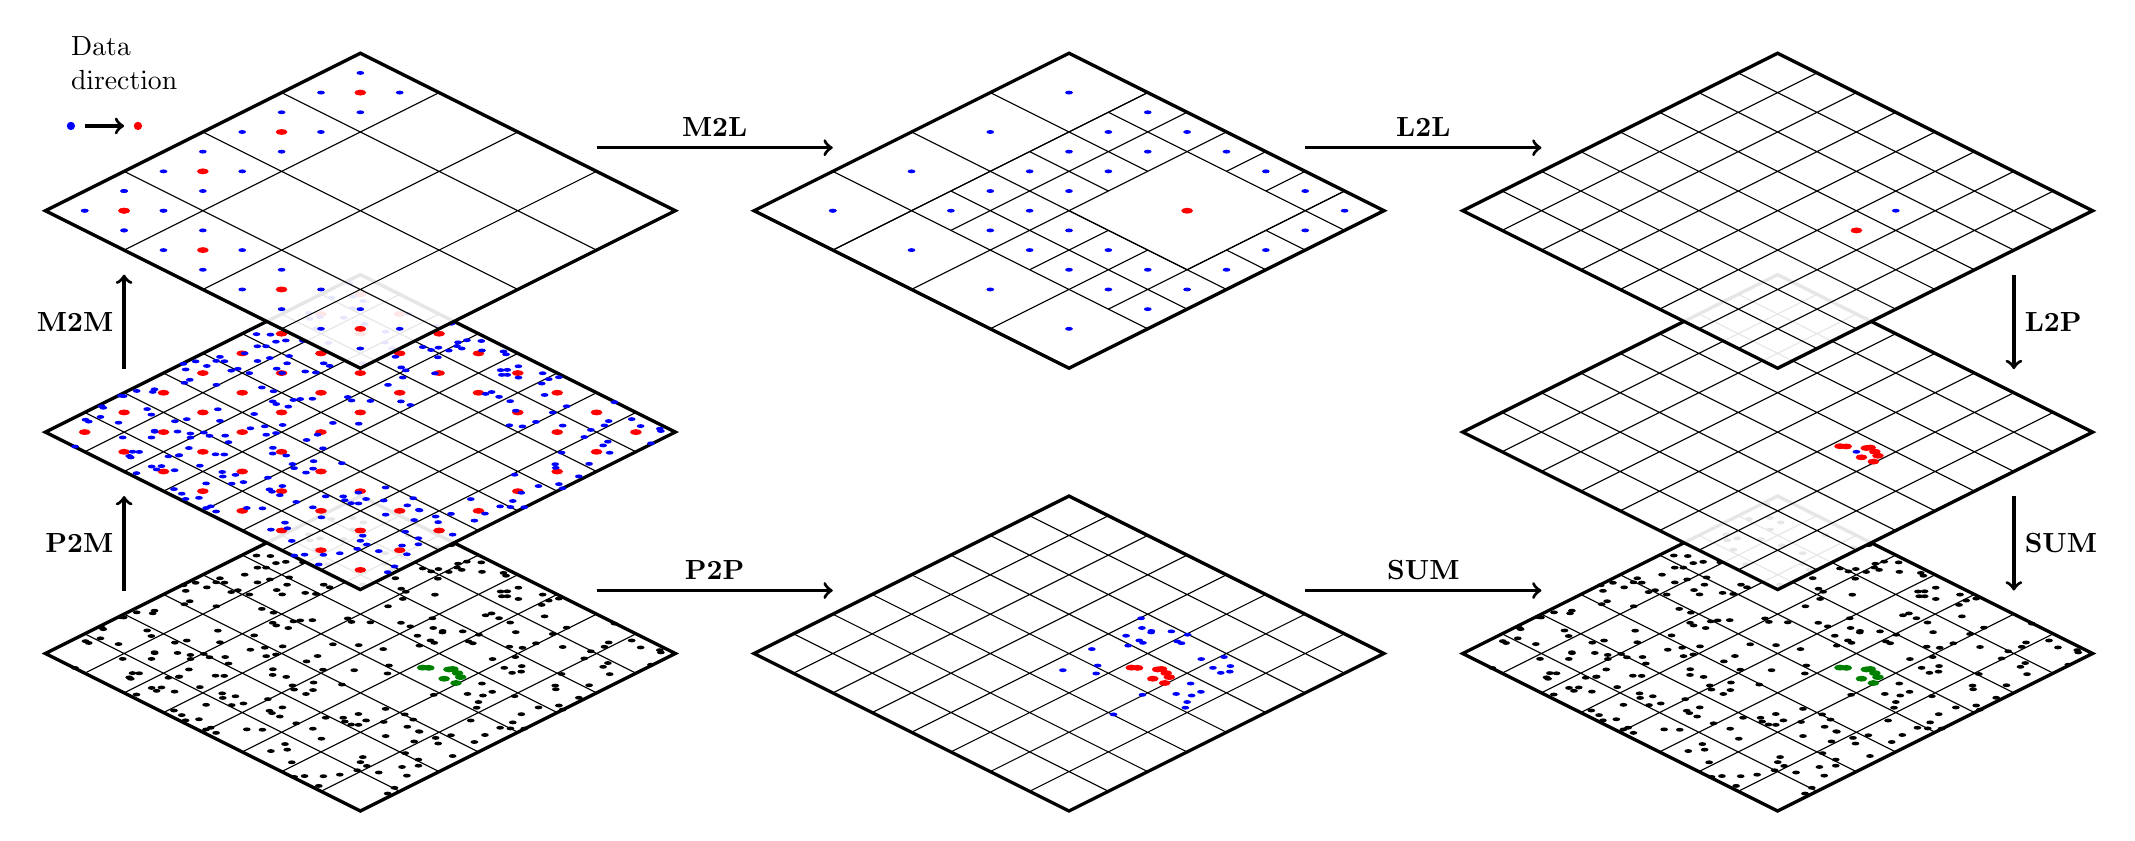
\begin{tikzpicture}
\def\nrand{300}
\def\seed{12}
\def\gridSize{5mm}
\def\gridTotal{4}
% Particles to Multipole
\pgfmathsetseed{\seed}
\begin{scope}[
   		yshift=0,every node/.append style={
    		yslant=0.5,xslant=-1},yslant=0.5,xslant=-1
    ]
    \fill[white,fill opacity=.9] (0,0) rectangle (4,4);
    \draw[black,very thick] (0,0) rectangle (4,4);
	\draw[step=\gridSize, black] (0,0) grid (\gridTotal,\gridTotal);
	\foreach \i in {1,2,...,\nrand}{
    	\pgfmathsetmacro{\x}{(rand)*2+2}
    	\pgfmathsetmacro{\y}{(rand)*2+2}
		% COLOR 
		\ifthenelse{\( \lengthtest{\x cm>2cm} \AND \lengthtest{\x cm<2.5cm} \)}
		{	
			\ifthenelse{ \( \lengthtest{\y cm>1cm} \AND \lengthtest{\y cm<1.5cm} \)}
			{\node at (\x,\y) [black!50!green,circle,fill,inner sep=.7pt,minimum size=3pt]{};}
			{\node at (\x,\y) [circle,fill,inner sep=.7pt]{};}
		}
		{\node at (\x,\y) [circle,fill,inner sep=.7pt]{};}
	}
\end{scope}
\pgfmathsetseed{\seed}
\begin{scope}[
   		yshift=80,every node/.append style={
    		yslant=0.5,xslant=-1},yslant=0.5,xslant=-1
    ]
    \fill[white,fill opacity=.9] (0,0) rectangle (4,4);
    \draw[black,very thick] (0,0) rectangle (4,4);
	\draw[step=5mm, black] (0,0) grid (\gridTotal,\gridTotal);
	\foreach \x in {0,1,...,7}{\foreach \y in {0,1,...,7}{
		\ifthenelse{\( \x<3 \OR \x>5 \)}
		{
			\node at (\x*\gridSize+\gridSize/2,\y*\gridSize+\gridSize/2)[red,circle,fill,inner sep=.7pt,minimum size=3pt]{};
		}
		{	\ifthenelse{ \( \y<1 \OR \y>3 \)}
			{
			\node at (\x*\gridSize+\gridSize/2,\y*\gridSize+\gridSize/2)[red,circle,fill,inner sep=.7pt,minimum size=3pt]{};	
			}{}
		}
	}}
	\foreach \i in {1,2,...,\nrand}{
    	\pgfmathsetmacro{\x}{(rand)*2+2}
    	\pgfmathsetmacro{\y}{(rand)*2+2}
    	\ifthenelse{\( \lengthtest{\x cm<1.5cm} \OR \lengthtest{\x cm>3cm} \)}
		{\node at (\x,\y) [blue,circle,fill,inner sep=.7pt]{};}
		{	\ifthenelse{ \( \lengthtest{\y cm<.5cm} \OR \lengthtest{\y cm>2cm} \)}
			{\node at (\x,\y) [blue,circle,fill,inner sep=.7pt]{};}
			{}
		}
  	}
\end{scope}
\begin{scope}[
   		yshift=160,every node/.append style={
    		yslant=0.5,xslant=-1},yslant=0.5,xslant=-1
    ]
    \fill[white,fill opacity=.9] (0,0) rectangle (4,4);
    \draw[black,very thick] (0,0) rectangle (4,4);
	\draw[step=10mm, black] (0,0) grid (4,4);
	\foreach \x in {0,1}{\foreach \y in {0,...,7}{
		\node at (\x*\gridSize+\gridSize/2,\y*\gridSize+\gridSize/2)[blue,circle,fill,inner sep=.7pt]{};
	}}
	\foreach \x in {0,...,7}{\foreach \y in {6,7}{
		\node at (\x*\gridSize+\gridSize/2,\y*\gridSize+\gridSize/2)[blue,circle,fill,inner sep=.7pt]{};
	}}

	\foreach \x in {0}{\foreach \y in {0,...,3}{				  
		\node at (\x*\gridSize*2+\gridSize,\y*\gridSize*2+\gridSize) [red,circle,fill,inner sep=.7pt,minimum size=3pt]{};
	}}
	\foreach \x in {0,...,3}{\foreach \y in {3}{				  
		\node at (\x*\gridSize*2+\gridSize,\y*\gridSize*2+\gridSize) [red,circle,fill,inner sep=.7pt,minimum size=3pt]{};
	}}
\end{scope}

%PARTICLES TO PARTICLES
\pgfmathsetseed{\seed}
\begin{scope}[
   		yshift=0,xshift=9cm,every node/.append style={
    		yslant=0.5,xslant=-1},yslant=0.5,xslant=-1
    ]
    \fill[white,fill opacity=.9] (0,0) rectangle (4,4);
    \draw[black,very thick] (0,0) rectangle (4,4);
	\draw[step=5mm, black] (0,0) grid (4,4);
	\foreach \i in {1,2,...,\nrand}{
    	\pgfmathsetmacro{\x}{(rand)*2+2}
    	\pgfmathsetmacro{\y}{(rand)*2+2}
    	\ifthenelse{\( \lengthtest{\x cm>1.5cm} \AND \lengthtest{\x cm<3cm} \)}
		{	
			\ifthenelse{ \( \lengthtest{\y cm>.5cm} \AND \lengthtest{\y cm<2cm} \)}
			{
				% COLOR 
				\ifthenelse{\( \lengthtest{\x cm>2cm} \AND \lengthtest{\x cm<2.5cm} \)}
				{	
					\ifthenelse{ \( \lengthtest{\y cm>1cm} \AND \lengthtest{\y cm<1.5cm} \)}
					{\node at (\x,\y) [red,circle,fill,inner sep=.7pt,minimum size=3pt]{};}
					{\node at (\x,\y) [blue,circle,fill,inner sep=.7pt]{};}
				}
				{\node at (\x,\y) [blue,circle,fill,inner sep=.7pt]{};}
			}{}
		}{}
    	%\node at (\x,\y) [circle,fill,inner sep=.7pt]{};
  	}
\end{scope}
%MULTIPOLE TO MULTIPOLE
\begin{scope}[
   		yshift=160,xshift=9cm,every node/.append style={
    		yslant=0.5,xslant=-1},yslant=0.5,xslant=-1
    ]
    \fill[white,fill opacity=.9] (0,0) rectangle (4,4);
    \draw[black,very thick] (0,0) rectangle (4,4);
    \draw[step=10mm, black] (0,3) grid (4,4);
	\draw[step=10mm, black] (0,0) grid (1,3);
	\draw[step=5mm, black] (1,0) grid (2,3);
	\draw[step=5mm, black] (2,2) grid (4,3);
	\draw[step=5mm, black] (2,0) grid (4,.5);
	\draw[step=5mm, black] (3.5,0) grid (4,2);
	% add rectangle
	\draw[black] (2,.5) rectangle (3.5,2);
	% Big part 
	\foreach \x in {0}{\foreach \y in {0,...,3}{				  
		\node at (\x*\gridSize*2+\gridSize,\y*\gridSize*2+\gridSize) [blue,circle,fill,inner sep=.7pt]{};
	}}
	\foreach \x in {0,...,3}{\foreach \y in {3}{				  
		\node at (\x*\gridSize*2+\gridSize,\y*\gridSize*2+\gridSize) [blue,circle,fill,inner sep=.7pt]{};
	}}
	% Smaller one 
	\foreach \x in {2,3}{\foreach \y in {0,...,3}{
		\node at (\x*\gridSize+\gridSize/2,\y*\gridSize+\gridSize/2)[blue,circle,fill,inner sep=.7pt]{};
	}}

	\foreach \x in {2,...,7}{\foreach \y in {4,5}{
		\node at (\x*\gridSize+\gridSize/2,\y*\gridSize+\gridSize/2)[blue,circle,fill,inner sep=.7pt]{};
	}}

	\foreach \x in {7}{\foreach \y in {0,...,3}{
		\node at (\x*\gridSize+\gridSize/2,\y*\gridSize+\gridSize/2)[blue,circle,fill,inner sep=.7pt]{};
	}}
	\foreach \x in {4,5,6}{\foreach \y in {0}{
		\node at (\x*\gridSize+\gridSize/2,\y*\gridSize+\gridSize/2)[blue,circle,fill,inner sep=.7pt]{};
	}}
	\node at (5*\gridSize+\gridSize/2,2*\gridSize+\gridSize/2) [red,circle,fill,inner sep=.7pt,minimum size=3pt]{};
\end{scope}

% Multipole to Particles 
\pgfmathsetseed{\seed}
\begin{scope}[
   		yshift=0,xshift=18cm,every node/.append style={
    		yslant=0.5,xslant=-1},yslant=0.5,xslant=-1
    ]
    \fill[white,fill opacity=.9] (0,0) rectangle (4,4);
    \draw[black,very thick] (0,0) rectangle (4,4);
	\draw[step=5mm, black] (0,0) grid (4,4);
	\foreach \i in {1,2,...,\nrand}{
    	\pgfmathsetmacro{\x}{(rand)*2+2}
    	\pgfmathsetmacro{\y}{(rand)*2+2}
		% COLOR 
		\ifthenelse{\( \lengthtest{\x cm>2cm} \AND \lengthtest{\x cm<2.5cm} \)}
		{	
			\ifthenelse{ \( \lengthtest{\y cm>1cm} \AND \lengthtest{\y cm<1.5cm} \)}
			{\node at (\x,\y) [black!50!green,circle,fill,inner sep=.7pt,minimum size=3pt]{};}
			{\node at (\x,\y) [circle,fill,inner sep=.7pt]{};}
		}
		{\node at (\x,\y) [circle,fill,inner sep=.7pt]{};}
	}
\end{scope}
\pgfmathsetseed{\seed}
\begin{scope}[
   		yshift=80,xshift=18cm,every node/.append style={
    		yslant=0.5,xslant=-1},yslant=0.5,xslant=-1
    ]
    \fill[white,fill opacity=.9] (0,0) rectangle (4,4);
    \draw[black,very thick] (0,0) rectangle (4,4);
	\draw[step=5mm, black] (0,0) grid (4,4);

	\foreach \i in {1,2,...,\nrand}{
    	\pgfmathsetmacro{\x}{(rand)*2+2}
    	\pgfmathsetmacro{\y}{(rand)*2+2}
    	\ifthenelse{\( \lengthtest{\x cm>1.5cm} \AND \lengthtest{\x cm<3cm} \)}
		{	
			\ifthenelse{ \( \lengthtest{\y cm>.5cm} \AND \lengthtest{\y cm<2cm} \)}
			{
				% COLOR 
				\ifthenelse{\( \lengthtest{\x cm>2cm} \AND \lengthtest{\x cm<2.5cm} \)}
				{	
					\ifthenelse{ \( \lengthtest{\y cm>1cm} \AND \lengthtest{\y cm<1.5cm} \)}
					{\node at (\x,\y) [red,circle,fill,inner sep=.7pt,minimum size=3pt]{};}
					{}
				}{}
			}{}
		}{}
	}
	\node at (4*\gridSize+\gridSize/2,2*\gridSize+\gridSize/2) [blue,circle,fill,inner sep=.7pt]{};
\end{scope}
%% MULTIPOLE TO LOCAL
\begin{scope}[
   		yshift=160,xshift=18cm,every node/.append style={
    		yslant=0.5,xslant=-1},yslant=0.5,xslant=-1
    ]
    \fill[white,fill opacity=.9] (0,0) rectangle (4,4);
    \draw[black,very thick] (0,0) rectangle (4,4);
	\draw[step=5mm, black] (0,0) grid (4,4);
	\node at (4*\gridSize+\gridSize/2,2*\gridSize+\gridSize/2) [red,circle,fill,inner sep=.7pt,minimum size=3pt]{};

	\node at (5*\gridSize+\gridSize/2,2*\gridSize+\gridSize/2) [blue,circle,fill,inner sep=.7pt]{};
\end{scope}
% ARROWS AND TEXT
\draw[->,very thick] (-3,2.8) -- (-3,4) node[midway,left] {\textbf{P2M}};
\draw[->,very thick] ([yshift=80]-3,2.8) -- ([yshift=80]-3,4) node[midway,left] {\textbf{M2M}};

\draw[->,very thick] ([yshift=160]3,2.8) -- ([yshift=160]6,2.8) node[midway,above] {\textbf{M2L}};
\draw[->,very thick] ([yshift=160,xshift=9cm]3,2.8) -- ([yshift=160,xshift=9cm]6,2.8) node[midway,above] {\textbf{L2L}};

\draw[<-,very thick] ([yshift=80]21,2.8) -- ([yshift=80]21,4) node[midway,right] {\textbf{L2P}};
\draw[<-,very thick] (21,2.8) -- (21,4) node[midway,right] {\textbf{SUM}};

\draw[->,very thick] (3,2.8) -- (6,2.8) node[midway,above] {\textbf{P2P}};
\draw[->,very thick] ([xshift=9cm]3,2.8) -- ([xshift=9cm]6,2.8) node[midway,above] {\textbf{SUM}};


\draw[->,very thick] (-3.5,8.7cm) node[xshift=-5pt,blue,circle,fill,inner sep=.7pt,minimum size=3pt] (a) {} -- 
 (-3,8.7cm) node[xshift=5pt,red,circle,fill,inner sep=.7pt,minimum size=3pt] (b) {};
\node[align=left] at (-3,9.5cm) {Data\\direction};


\end{tikzpicture}
}
\caption{Fast Multipole Method schematics. Particles to Multipole (P2M), Multipole to Multipole (M2M), Multipole to Particles (M2P), Multipole to Local (M2L), Local to Local (L2L) and Particles to Particles (P2P). Schematic inspired from \cite{yokota2011treecode}}
\end{figure}

This method is based on Taylor series.
The gravitation function of equation~\ref{eq:gravitation} can be approximate on a particle at position $\vec{r}$ by the gravitation computed at the centroid at position $\vec{r_c}$: 
\begin{equation}
 \vec{f}(\vec{r}) = \vec{f}(\vec{r_c}) + ||\frac{\partial\vec{f}}{\partial\vec{r}}||\cdot (\vec{r} - \vec{r_c}) + \frac{1}{2} (\vec{r}-\vec{r_c})^\intercal \cdot   ||\frac{\partial\vec{f}}{\partial\vec{r} \partial\vec{r}}|| \cdot (\vec{r} - \vec{r_c})
 \end{equation}

 From equation~\ref{eq:gravitation} we compute the term $||\frac{\partial\vec{f}}{\partial\vec{r}}||$:s
 \begin{equation}
\frac{\partial\vec{f}}{\partial\vec{r}} =
- \sum_p \frac{m_p}{|\vec{r_c}-\vec{r_p}|^3}
\begin{bmatrix}
1 - \frac{3(x_c-x_p)(x_c-x_p)}{|\overline{r_c}-\overline{r_p}|^2} & -\frac{3(y_c-y_p)(x_c-x_p)}{|\overline{r_c}-\overline{r_p}|^2}  & -\frac{3(z_c-z_p)(x_c-x_p)}{|\vec{r_c}-\vec{r_p}|^2}  \\
-\frac{3(x_c-x_p)(y_c-y_p)}{|\vec{r_c}-\vec{r_p}|^2}  & 1 - \frac{3(y_c-y_p)(y_c-y_p)}{|\vec{r_c}-\vec{r_p}|^2} &  -\frac{3(z_c-z_p)(y_c-y_p)}{|\vec{r_c}-\vec{r_p}|^2}\\
- \frac{3(x_c-x_p)(z_c-z_p)}{|\vec{r_c}-\vec{r_p}|^2}   &  -\frac{3(y_c-y_p)(z_c-z_p)}{|\vec{r_c}-\vec{r_p}|^2} &  1- \frac{3(z_c-z_p)(z_c-z_p)}{|\vec{r_c}-\vec{r_p}|^2} \\
\end{bmatrix}
 \end{equation}

And we propose a compact version of the matrix with: 
 
\begin{equation}
 ||\frac{\partial f^a}{\partial r^b}|| = -\sum_c \frac{m_c}{|\vec{r}-\vec{r_c}|^3} \Big[ \delta_{ab} - \frac{3.(r^a-r_c^a)(r^b-r_c^b)}{|\vec{r}-\vec{r_c}|^2} \Big] 
\end{equation}

With $\delta_{ab}$ the kronecker delta:
\begin{equation}
\delta_{ab} = 
\begin{cases}
    1, & \text{if $a = b$}.\\
    0, & \text{if $a\neq b$}.
  \end{cases}
\end{equation}

We note that $a$ and $b$ variate from 0 to 2 and $r^0=x$, $r^1=y$, and $r^2=z$ as usual sense. 

For the term $||\frac{\partial\vec{f}}{\partial\vec{r} \partial\vec{r}}||$ we give the compact version by:
\begin{equation}
||\frac{\partial^2 f^a}{\partial r^b \partial r^c}|| =
- \sum_c \frac{3 m_c}{|\vec{r}-\vec{r_c}|^5} \left[\frac{5(r^a-r_c^a)(r^b-r_c^b)(r^c-r_c^c)}{|\vec{r}-\vec{r_c}|^2} - \left( \delta_{ab} (r^c-r_c^c)+\delta_{bc} (r^a-r_c^a)+\delta_{ac} (r^b-r_c^b) \right) \right] 
 \end{equation} 

 \begin{figure}
 \end{figure}

The method is summed up in figure with the different equations.
We consider Centers Of Mass, COM, to be the centroid of particles based on their position. 
In several steps the information is first transmitted to the COMs, computing their position and mass. 


\subsection{Problems} 
The previous equations are generic and describe the behavior of SPH method. 
In order to check our 

\subsubsection{Sod shock tube}

\subsubsection{Sedov blast wave}

\subsubsection{Fluid flow}

\subsubsection{Astrophysics: neutron stars coalescence}

The final aim of our tests is to simulate astrophysical events. 
We are interested in one of the most important event recently discovered. 
Last year the Laser Interferometer Gravitational Wave, LIGO, detected the first gravitational wave generated by binary neutron stars merging \cite{abbott2017gw170817} and also more complexes event with Binary Black Holes coalescence in \cite{abbott2017gw170814}.


\paragraph{Solving Lane-Emden Equation}

We need to determine the density function based on the radius. 

As we consider the star as a polytropic fluid, we use the equation of Lane-Emden which is a form of the Poisson equation: 

\begin{equation}\label{eq_LaneEmden}
  \frac{d^2\theta}{d \xi^2}+ \frac{2}{\xi}\frac{d\theta}{d\xi}+\theta^n = 0
\end{equation}

With $\xi$ and $\theta$ two dimensionless variables. 
There is only exact solutions for a polytropic index $n = 0.5$, $1$ and $2$.
In our work we use a polytropic index of $1$ which can correspond to a NS simulation.

For $n=1$ the solution of equation \ref{eq_LaneEmden} is: 

\begin{equation}
\theta(\xi)=\frac{sin(\xi)}{\xi}
\end{equation}

We note $\xi_1 = \pi$, the first value of $\xi$ as $\theta(\xi) = 0$.
$\theta(\xi)$ is also defined as: 
\begin{equation}
 \theta(\xi) = \Big(\frac{\rho(\xi)}{\rho_c}\Big)^{\frac{1}{n}}  = \frac{\rho(\xi)}{\rho_c}
\end{equation}

With $\rho_c$ the internal density of the star and $\rho$ the density at a determined radius. $\xi$ is defined as:  
$$ \xi = Ar = \sqrt{\frac{4\pi G}{K(n+1)}\rho_c^{(n-1)/n}} \times r = \sqrt{\frac{2\pi G}{K}}\times r \mbox{ (for } n=1 \mbox{)}$$

With $K$ a proportionality constant.

From the previous equations we can write the stellar radius $R$ as:
\begin{equation}
R = \sqrt{\frac{K(n+1)}{4\pi G}}\rho_c^{(1-n)/2}\xi_1 = \sqrt{ \frac{K}{2\pi G} } \times \xi_1
\end{equation} 

(We note that for $n=1$ the radius does not depend of the central density.)

If, for example, we use dimensionless units as $G=R=M=1$ (for the other results we use CGS with $G = 6.674 \times 10^{-8} cm^3g^{-1}s^{-2}$) 
We can compute K as: 
\begin{equation}
\label{eq:constant}
K = \frac{R^2  2 \pi G}{\xi_1^2}
\end{equation}

\begin{center}

\begin{tabular}{c|c|c|c|c|}
 & $NS_1$ & $NS_2$ & $NS_3$ & $NS_4$ \\ 
\hline 
Radius (cm) & $R=G=M=1$ & 1500000 & 1400000 & 960000 \\ 
\hline 
K & 0.636619 & 95598.00 & 83576.48 & 39156.94\\ 
\hline 
\end{tabular}

\end{center} 

Then we deduce the density function of $r$ as :

$$\rho(\xi) = \frac{sin(A\times r)}{A \times r} \times \rho_c \mbox{ with } A = \sqrt{\frac{2\pi G}{K}}
$$

As we know the total Mass $M$, the radius $R$ and the gravitational constant $G$ we can compute the central density as: 

$$ \rho_c = \frac{M A^3}{4 \pi (sin(AR)-ARcos(AR)) } $$

Then we normalize the results to fit $R = M = G = 1$: $K' = K/(R^2G) $, $m_i' = m_i/M $, $h_i' = h_i / R$, $\vec{x_i}' = \vec{x_i}/R$ 

\section{Conclusion}


%%%%%%%%%%%%%%%%%%%%%%%%%%%%%%%%%%%%%%%%%%%%%%%%%%%%%%%%%%%%%%%%%%%%%
%                                                                   %
% CHAPTER ONE, Computation wall                                     % 
%                                                                   %
%%%%%%%%%%%%%%%%%%%%%%%%%%%%%%%%%%%%%%%%%%%%%%%%%%%%%%%%%%%%%%%%%%%%%

%%%%%%%%%%%%%%%%%%%%%%%%%%%%%%%%%%%%%%%%%%%%%%%%%%%%%%%%%%%%%%%%%%%%%
%                                                                   %
% CHAPTER FIVE: COMPUTATIONAL WALL: LANGFORD PROBLEM                %
%                                                                   %
%%%%%%%%%%%%%%%%%%%%%%%%%%%%%%%%%%%%%%%%%%%%%%%%%%%%%%%%%%%%%%%%%%%%%

\chapter{Computational Wall: Langford Problem}

\section{Introduction}
Our aim is to determine the behavior of accelerators compared to classical processor in case of irregular-computationally heavy problems.
For this purpose we choose the Langford problem which is an academic problem of combinatorial counting.
We show the optimizations made to the regular processor algorithm to efficiently implement this application on GPU. 
We compare the two approaches from classical processor to GPU implementation. 
The results are then presented to show the acceleration using the whole ROMEO supercomputer.
This study shows two approaches to the Langford problem.
The Miller's algorithm, irregular tree backtracking and the the Godfrey's method which is use in order to beat a time record on this problem.\\

C. Dudley Langford gave his name to a classic permutation problem ~\cite{Gard56, Simp83}.  
While observing his son manipulating blocks of different colors, he noticed that it was possible to arrange three pairs of different colored blocks (yellow, red and blue) in such a way that only one block separates the red pair - noted as pair 1 - , two blocks separate the blue pair - noted as pair 2 - and finally three blocks separate the yellow one - noted as pair 3 - , see figure~\ref{fig:lang}.\\

\begin{figure}[htbp]    
\begin{center}    
%\includegraphics[scale=0.45]{\locpath/figures/langford/lgf_cubes}   
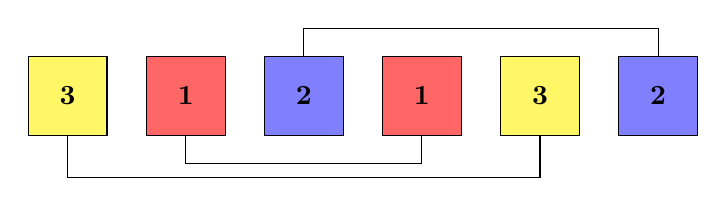
\begin{tikzpicture}
\node (rect) at (0,0) [fill=yellow!60,draw,minimum width=1cm,minimum height=1cm] (p3_1) {\textbf{3}};
\node (rect) at (1.5,0) [fill=red!60,draw,minimum width=1cm,minimum height=1cm] (p1_1) {\textbf{1}};
\node (rect) at (3,0) [fill=blue!50,draw,minimum width=1cm,minimum height=1cm] (p2_1) {\textbf{2}};
\node (rect) at (4.5,0) [fill=red!60,draw,minimum width=1cm,minimum height=1cm] (p1_2) {\textbf{1}};
\node (rect) at (6,0) [fill=yellow!60,draw,minimum width=1cm,minimum height=1cm] (p3_2) {\textbf{3}};
\node (rect) at (7.5,0) [fill=blue!50,draw,minimum width=1cm,minimum height=1cm] (p2_2) {\textbf{2}};
\draw (p3_1.south) -- ([yshift=-15pt]p3_1.south) -- ([yshift=-15pt]p3_2.south) -- (p3_2.south) ;
\draw (p2_1.north) -- ([yshift=10pt]p2_1.north) -- ([yshift=10pt]p2_2.north) -- (p2_2.north) ;
\draw (p1_1.south) -- ([yshift=-10pt]p1_1.south) -- ([yshift=-10pt]p1_2.south) -- (p1_2.south) ;
\end{tikzpicture}  
\end{center}
\caption{L(2,3) arrangement} \label{fig:lang}  
\end{figure}
  
This problem has been generalized to any number $n$ of colors and any number $s$ of blocks having the same color. 
$L(s,n)$ consists in searching for the number of solutions to the Langford problem, up to a symmetry. % ... excepted symmetric ones. 
In November 1967, Martin Gardner presented $L(2,4)$ (two cubes and four colors) as being part of a collection of small mathematical games and he stated that $L(2,n)$ has solutions for all $n$ such that:
\begin{equation}
\text{ solutions for: }
\begin{cases}
n= 4k \\ 
n = 4k-1
\end{cases}
 k \in \mathbb{N}^+
\end{equation}
The central resolution method consists in placing the pairs of cubes, one after the other, on the free places and backtracking if no place is available (see figure~\ref{backtrack} for detailed algorithm).

\begin{table}[t!]
\centering
\[
\begin{tabular}{c r r r}
  \hline
  Instance & Solutions & Method & Computation time\\
  \hline
  \hline
  L(2,3) & 1 &  Miller algorithm & - \\
  L(2,4) & 1 & & - \\ 
  ... & ... & & ...  \\
  L(2,16) & 326,721,800 & & 120 hours  \\
  %\cline{1-3}
  L(2,19) & 256,814,891,280 & & 2.5 years (1999) DEC Alpha \\
  \hline
  \hline
  L(2,20) & 2,636,337,861,200 & Godfrey algorithm & 1 week \\
  %\cline{1-3}
  L(2,23) & 3,799,455,942,515,488 & &  4 days with CONFIIT \\
  %\cline{1-3}
  L(2,24) & 46,845,158,056,515,936 & & 3 months with CONFIIT \\
  L(2,27) & 111,683,611,098,764,903,232 & & 2 days on ROMEO \\
  L(2,28) & 1,607,383,260,609,382,393,152 & & 23 days on ROMEO \\
  \hline
\end{tabular}
\]
\caption{Solutions and time for Langford problem using different methods}
\label{tab:result_base}
\end{table}

The Langford problem has been approached in different ways: discrete mathematics results, specific algorithms, specific encoding, constraint satisfaction problem (CSP), inclusion-exclusion~\ldots~\cite{Mil00,apes-26,Smi00,larsen2009counting}.
In 2004, the last solved instance, $L(2,24)$, was computed by our team \cite{CReSTIC-711} using a specific algorithm. 
Table \ref{tab:result_base} presents the latest results and number of solutions. 
$L(2,27)$ and $L(2,28)$ have just been computed but no details were given. 

The most efficient known algorithms are: the Miller backtrack method, the Godfrey algebraic method and the Larsen inclusion-exclusion method.
The Miller one is based on backtracking and can be modeled as a CSP; it allowed us to move the limit of explicits solutions building up to $L(2,21)$ but combinatorial explosion did not allow us to go further. 
Then, we use the Godfrey method to achieve $L(2,24)$ more quickly and then recompute $L(2,27)$ and $L(2,28)$, presently known as the last instances.
The Larsen method is based on inclusion-exclusion \cite{larsen2009counting}; although this method is effective, practically the Godfrey one is better. 
The latest known work on the Langford Problem is a GPU implementation proposed in \cite{ASS_LGF} in 2015. Unfortunately this study does not provide any performance considerations but just gives the number of solution of $L(2,27)$ and $L(2,28)$.

\section{Miller algorithm}

In this part we present our multi-GPU cluster implementation of the Miller's algorithm. 
This algorithm is very irregular and the repartition have to be done at runtime on our accelerators. 

First, we introduce the backtrack method. 
Then we present our implementation in order to fit the GPUs architecture. 
The last section presents our results. 

\subsection{CSP}

Combinatorial problems are NP-complete \cite{GJ79} and can be described as SATISFIABILITY problems (SAT) using a polynomial transformation. 
They can be transformed into CSP formalism.
A Constraint Satisfaction Problem (CSP), first introduced by Montanari \cite{Mon74}, is defined as a triple $<X,D,C>$ where:
\begin{equation}
\begin{cases}
X=\{X_1,...,X_n\}\text{: a finite set of variables} \\ 
D=\{D_1,...,D_n\}\text{: their finite domains of values}\\
C=\{C_1,...,C_p\}\text{: a finite set of constraints}
\end{cases}
\end{equation}

The goal in this formalism is to assign values in $D$ to $n$-uple $X$ respecting all the $C$ $p$-uple constraints.
This approach is a large field of research. \cite{arbelaez2014gpu} developed \textit{local search} and compares GPU to CPU. 
This first work brings to light that GPU is a real contributor to the global computation speed. \cite{campeotto2014exploring} proposes a solver using \textit{propagator} on a GPU architecture to solve CSP problems. 
\cite{jenkins2011lessons} cares about GPU weak points, loading bandwidth and global memory latency.

%\subsection{CSP parallel resolution}
%\label{sec:CSP_resolution}

Considering a basic approach, combinatorial problems formed into CSP can be represented as a tree search. Each level corresponds to a given variable, with values in its domain. Leaves of the tree correspond to a complete assignment (all variables are set). If it meets all the constraints this assignment is called an acceptor state. Depending on the constraints set, the satisfiability evaluation can be made either on complete or partial assignment.
%
%There are many ways to browse the tree and find the solutions: \emph{backtracking}, \emph{forward-checking}, \emph{backjumping}, etc. 
%We limit our method to the naive \emph{backtrack} resolution. We chose to evaluate the variables and their values in a static order; in a depth-first manner, the solution is built incrementally and if a partial assignment can be aborted, the branch is cut. A solution is found each time a leaf is reached.
%% presents a backtrack search with the previous CSP representation.
%
%The recommendation for performance on GPU accelerator is to use non test-based programs.
%Due to its irregularity, the basic \emph{backtracking} algorithm is suppose not to suit the GPU architecture.
%Thus a vectorized version is given when evaluating the assignments at the leaves' level, with one of the two following ways: assignments can be prepared on each tree node or totally set on final leaves before testing the satisfiability of the built solution, Fig.\ref{fig:algos}.
%
%\begin{figure}[htbf]
%\begin{minipage}[b]{0.45\linewidth}
%\begin{verbatim}
%for variable_1 
%   assignment
%   for variable_2
%      assignment
%      ...
%         for variable_n
%            assignment
%            test
%\end{verbatim}
%\end{minipage}
%\begin{minipage}[b]{0.45\linewidth}
%\begin{verbatim}
%for variable_1 
%   for variable_2
%   ...
%      for variable_n
%         assignments
%         test
%         
%         
%\end{verbatim}
%\end{minipage} 
%\caption{CSP regularized algorithms}
%\label{fig:algos}
%\end{figure} 
%
%With this method it is necessary to browse the entire tree but this requires using all the search space and it is too time-consuming.
%
%In order to overcome this we divide the work between CPU and GPU. The CPU generates some levels of the tree and creates tasks. Then GPU and CPU cores divide up the workload in order to achieve the generation on the latest levels of the tree. With this method, inconsistent branches can be cut on highest level and GPU/CPU cores only compute possibly consistent tasks.
%
%This representation enables a server-client model to distribute the tasks: the server generates independent sub-problems at a chosen depth in the tree, treated by clients. 
%Each client decomposes the sub-problem into tasks, distributed over the GPU/CPU cores, Fig.\ref{fig:parallel}.
%
%\begin{figure}[htbf]
%\centering 
%\includegraphics[scale=0.9]{figures/graphe_repartition}   
%\caption{Server client distribution} \label{fig:parallel}    
%\end{figure} 
%
%With this method numerous branches have been cut from the main tree during generation stage and GPU/CPU tasks are faster due to their lower depth. Despite the combinatorial explosion of this kind of problem, we can consider solving CSP in a massively parallel manner on multiGPU clusters.

\subsection{Backtrack resolution}

As presented above the Langford problem is known to be a highly irregular combinatorial problem. 
We first present here the general tree representation and the ways we regularize the computation for GPUs.
Then we show how to parallelize the resolution over a multi-GPU cluster.

\subsubsection{Langford's problem tree representation}
\label{sec:LGF_resolution}
%In~\cite{HKS02}, we propose to formalize the Langford problem as a CSP  ({\it Constraint Satisfaction Problem}), first introduced by Montanari in \cite{Mon74}, and show that an efficient parallel resolution is possible. 
As explained, CSP formalized problems can be transformed into tree evaluations. %represented as trees. 
%The tree Here we intend to develop a specific algorithm taking into account the conclusion of our previous studies (memory management of memory and load balance) and transfer the tasks resolution into GPUs.\\
%\begin{figure}[htb]
%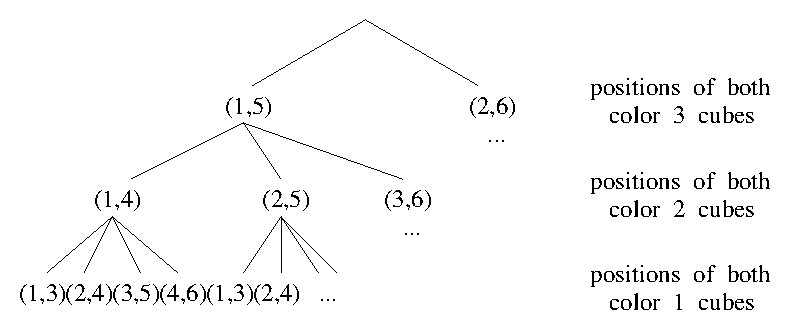
\includegraphics[scale=.65]{\locpath/figures/langford/arbre_en}
%\end{figure}
\begin{figure}[t!]
\centering
\resizebox {\columnwidth} {!} {
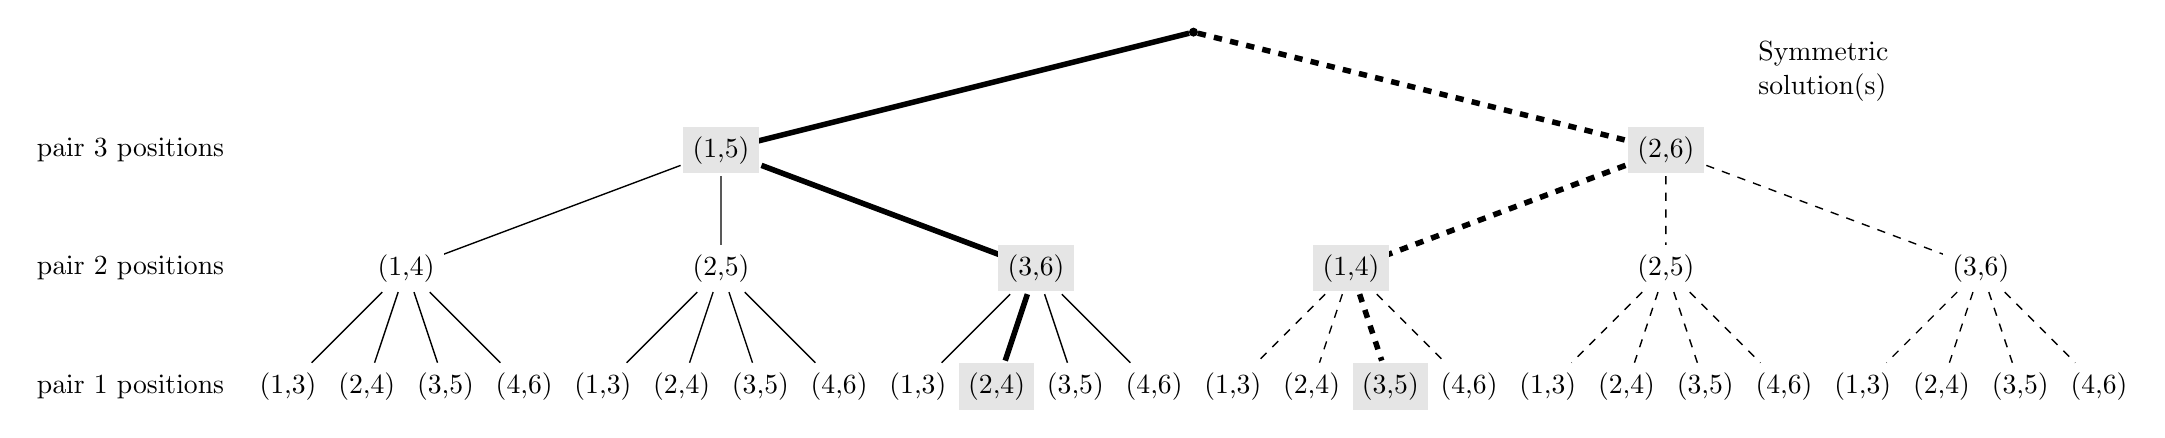
\begin{tikzpicture}[sibling distance=12cm]
\node at (-13.5,-1.5) {pair 3 positions};
\node at (-13.5,-3) {pair 2 positions};
\node at (-13.5,-4.5) {pair 1 positions};
\node [align=left] at (8,-.5) {Symmetric\\solution(s)};
\node  [circle,draw,fill,inner sep=1] {}
  child [line width=2pt] { [sibling distance=4cm] node [fill=black!10] {(1,5)}
    child [line width=.5pt] { [sibling distance=10mm] node [fill=white] {(1,4)}
      child {node {(1,3)}}
      child {node {(2,4)}}
      child {node {(3,5)}}
      child {node {(4,6)}}
    }
    child [line width=.5pt] { [sibling distance=10mm] node [fill=white] {(2,5)}
      child {node {(1,3)}}
      child {node {(2,4)}}
      child {node {(3,5)}}
      child {node {(4,6)}}
    }
    child { [sibling distance=10mm] node [fill=black!10] {(3,6)}
      child [line width=.5pt] {node {(1,3)}}
      child {node [fill=black!10] {(2,4)}}
      child [line width=.5pt] {node {(3,5)}}
      child [line width=.5pt] {node {(4,6)}}
    }
  }
  child [dashed,line width=2pt] { [sibling distance=4cm] node [fill=black!10] {(2,6)}
    child { [sibling distance=10mm] node [fill=black!10] {(1,4)}
      child [line width=.5pt] {node {(1,3)}}
      child [line width=.5pt] {node {(2,4)}}
      child {node [fill=black!10] {(3,5)}}
      child [line width=.5pt] {node {(4,6)}}
    }
    child [line width=.5pt] { [sibling distance=10mm] node [fill=white] {(2,5)}
      child {node {(1,3)}}
      child {node {(2,4)}}
      child {node {(3,5)}}
      child {node {(4,6)}}
    }
    child [line width=.5pt] { [sibling distance=10mm] node [fill=white] {(3,6)}
      child {node {(1,3)}}
      child {node {(2,4)}}
      child {node {(3,5)}}
      child {node {(4,6)}}
    }
  }
;
\end{tikzpicture}
}
\caption{Search tree for $L(2,3)$}
\label{fig:arbre}
\end{figure}
In order to solve $L(2,n)$, we consider a tree of height $n$: see example of $L(2,3)$ in figure~\ref{fig:arbre}.

\begin{itemize}   
\item[-] Every level of the tree corresponds to a color.
\item[-] Each node of the tree corresponds to the placement of a pair of cubes without worrying about the other colors. Color $p$ is represented at depth $n-p+1$, where the first node corresponds to the first possible placement (positions 1 and $p+2$) and $i^{th}$ node corresponds to the placement of the first cube of color $p$ in position $i, \ i \in [1, \ 2n-1-p]$.
\item[-] Solutions are leaves generated without any placement conflict.
\item[-] As we consider the solution up to a symmetry, the left part is represented dashed and is in fact not traversed.
\end{itemize}

There are many ways to browse the tree and find the solutions: \emph{backtracking}, \emph{forward-checking}, \emph{backjumping}, etc \cite{prosser93hybrid}. 
We limit our study to the naive \emph{backtrack} resolution and choose to evaluate the variables and their values in a static order; in a depth-first manner, the solutions are built incrementally and if a partial assignment can be aborted, the branch is cut. A solution is found each time a leaf is reached.
% presents a backtrack search with the previous CSP representation.

The recommendation for performance on GPU accelerators is to use non test-based programs.
Due to its irregularity, the basic \emph{backtracking} algorithm, presented on figure~\ref{backtrack}, is not supposed to suit the GPU architecture.
Thus a vectorized version is given when evaluating the assignments at the leaves' level, with one of the two following ways: assignments can be prepared on each tree node or totally set on final leaves before testing the satisfiability of the built solution (figure~\ref{regularized}).

\begin{figure}[t!]
\begin{minipage}[b]{0.45\linewidth}
\footnotesize
\begin{verbatim}
while not done do
 test pair            <- test
 if successful then 
   if max depth then
     count solution
     higher pair	                  
   else
     lower pair       <- remove
 else
   higher pair        <- add
\end{verbatim}
\caption{Backtrack algorithm}\label{backtrack}
\end{minipage}
\begin{minipage}[b]{0.45\linewidth}
\footnotesize
\begin{verbatim}
for pair 1 positions
  assignment                   <- add
  for pair 2 positions
    assignment                 <- add
    for ...
      for pair n positions
        assignment             <- add
        if final test ok then  
          count solution
\end{verbatim}
\caption{Regularized algorithm}\label{regularized}
\end{minipage}
\end{figure}

\subsubsection{Data representation}

\begin{figure}[t!]
\begin{minipage}[b]{0.40\linewidth}
\centering
\includegraphics[width=\columnwidth]{\locpath/figures/langford/positions_lgf}
\caption{ Bitwise representation of pairs positions in $L(2,3)$} \label{fig:comb1}
\end{minipage}
\hfill
\begin{minipage}[b]{0.55\linewidth}
\centering
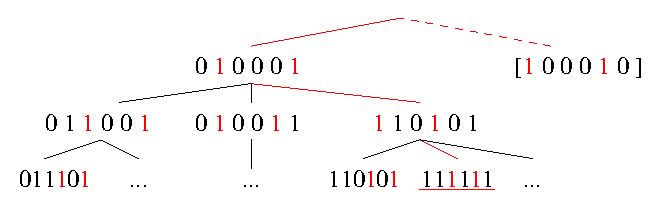
\includegraphics[width=\columnwidth]{\locpath/figures/langford/pos_lgf_v2}
\caption{Bitwise representation of the Langford $L(2,3)$ placement tree}\label{fig:pos_lgf}
\end{minipage}
\end{figure}

In order to count every Langford problem solution, we first identify all possible combinations for one color without worrying about the other ones. 
Each possible combination is coded within an integer, one bit to 1 corresponding to a cube presence, a 0 to its absence. This is what we called a \emph{mask}.
This way figure~\ref{fig:comb1} presents the possible combinations to place the one, two and three weight cubes for the $L(2,3)$ Langford instance.

Furthermore the masks can be used to evaluate the partial placements of a chosen set of colors: all the 1 correspond to occupied positions; the assignment is consistent \emph{iff} there are as many 1 as the number of cubes set for the assignment. 

With the aim to find solutions, we just have to go all over the tree and \emph{sum} one combination of each of the colors: a solution is found \emph{iff} all the bits of the sum are set to 1. 

Each route on the tree can be evaluated individually and independently; then it can be evaluated as a thread on the GPU.
This way the problem is massively parallel and can be, indeed, computed on GPU. figure~\ref{fig:pos_lgf} represents the tree masks' representation.

\subsubsection{Specific operations and algorithms}

Three main operations are required in order to perform the tree search. 
%The first one, allowing to check if a pair can be added to a given partial assignment, is only necessary for the original backtrack scheme.
%The second one, used for both backtrack and regularized methods, aims to add a pair to a given assignment. 
The first one, used for both backtrack and regularized methods, aims to add a pair to a given assignment. 
The second one, allowing to check if a pair can be added to a given partial assignment, is only necessary for the original backtrack scheme.
The last one is used for testing if a global assignment is an available solution: it is involved in the regularized version of the Miller algorithm.

\begin{figure}[t!]
\begin{minipage}[b]{0.5\linewidth}
\centering
\includegraphics[scale=.5]{\locpath/figures/langford/test_gen}
\caption{Testing and adding position} \label{fig:test_et}
\end{minipage}
\begin{minipage}[b]{0.5\linewidth}
\centering 
\includegraphics[scale=.75]{\locpath/figures/langford/graphe_repartition}   
\caption{Server client distribution} \label{fig:parallel} 
\end{minipage}
\end{figure}

\paragraph{Add a pair: }
Top of figure~\ref{fig:test_et} presents the way to add a pair to a given assignment.
With a \emph{binary OR}, the new mask contains the combination of the original mask and of the added pair.
This operation can be performed even if the position is not available for the pair (however the resulting mask is inconsistent). 

\paragraph{Test a pair position: }
On the bottom part of the same figure, we test the positioning of a pair on a given mask. 
For this, it is necessary to perform a \emph{binary AND} between the mask and the pair.
\begin{itemize}
	\item[] $=0$: \emph{success}, the pair can be placed here
	\item[] $\neq0$: \emph{error}, try another position
\end{itemize}

\paragraph{Final validity test: }
The last operation is for \emph{a posteriori} checking. For example the mask $101111$, corresponding to a leaf of the tree, is inconsistent and should not be counted among the solutions.
The final placement mask corresponds to a solution \emph{iff} all the places are occupied, which can be tested as $\neg mask = 0$. % \rightarrow solution$ else $inconsistent$.
%We performed a \emph{binary not} on the mask. If there is a zero, so the mask is inconsistent, result will be different of zero. If the mask is full of $1$, result is zero, so we can add one to the number of solutions.
\\

Using this data representation, 
we implemented both \emph{backtrack} and \emph{regularized} versions of the Miller algorithm, as presented in figure~\ref{backtrack} and \ref{regularized}.
% C'est là que je veux changer la structure ....
%: the original backtrack for CPU computation and the regularized one for GPUs.
%As we have seen above, the regularized algorithm is unsuitable due to combinatorial explosion, that is why we use the hybrid method on a distributed architecture.
\\
The next section presents the way we hybridize these two schemes in order to get an efficient parallel implementation of the Miller algorithm.

%%%%%%%%%%%%%%%%%%%%%%%%%%%%%%%%%%%%%%%%
\subsection{Hybrid parallel implementation}
\label{section:parallel_backtrack}
This part presents our methodology to implement Miller's method on a multiGPU cluster.

\paragraph{Tasks generation: }
In order to parallelize the resolution we have to generate tasks. 
Considering the tree representation, we construct tasks by fixing the different values of a first set of variables [pairs] up to a given level. Choosing the development level allows to generate as many tasks as necessary. This leads to a \textit{Finite number of Irregular and Independent Tasks} (\emph{FIIT} applications \cite{krajecki1999object}). 

\paragraph{Cluster parallelization: } 
The generated tasks are independent and we spread them in a client-server manner: a server generates them and makes them available for clients. As we consider the cluster as a set of CPU-GPU(s) machines, the clients are these machines. 
At the machines level, the role of the CPU is, first, to generate work for the GPU(s): it has to generate sub-tasks, by continuing the tree development as if it were a second-level server, and the GPU(s) can be considered as second-level client(s). \\
The sub-tasks generation, at the CPU level, can be made in parallel by the CPU cores. Depending on the GPUs number and their computation power the sub-tasks generation rhythm may be adapted, to maintain a regular workload both for the CPU cores and GPU threads: some CPU cores, not involved in the sub-tasks generation, could be made available for sub-tasks computing.\\
This leads to the 3-level parallelism scheme presented in figure~\ref{fig:parallel}, where $p$, $q$ and $r$ respectively correspond to: ($p$) the server-level tasks generation depth, ($q$) the client-level sub-tasks generation one, ($r$) the remaining depth in the tree evaluation, \textit{i.e.} the number of remaining variables to be set before reaching the leaves.  

\paragraph{\emph{Backtrack} and \emph{regularized} methods hybridization: } 
The Backtrack version of the Miller algorithm suits CPU execution and allows to cut branches during the tree evaluation, reducing the search space and limiting the combinatorial explosion effects. A regularized version had to be developed, since GPUs execution requires synchronous execution of the threads, with as few branching divergence as possible; however this method imposes to browse the entire search space and is too time-consuming. \\
We propose to hybridize the two methods in order to take advantage of both of them for the multiGPU parallel execution: 
for tasks and sub-tasks generated at sever and client levels, the tree development by the CPU cores is made using the backtrack method, cutting branches as soon as possible [and generating only possible tasks]; when computing the sub-tasks generated at client-level, the CPU cores involved in the sub-tasks resolution use the backtrack method and the GPU threads the regularized one. 

%With this method it is necessary to browse the entire tree but this requires using all the search space and it is too time-consuming.

%In order to overcome this we divide the work between CPU and GPU. The CPU generates some levels of the tree and creates tasks. Then GPU and CPU cores divide up the workload in order to achieve the generation on the latest levels of the tree. 
%With this method, inconsistent branches can be cut on highest level and GPU/CPU cores only compute possibly consistent tasks.

%This representation enables a server-client model to distribute the tasks: the server generates independent sub-problems at a chosen depth in the tree, treated by clients. 
%Each client decomposes the sub-problem into tasks, distributed over the GPU/CPU cores, Fig.~\ref{fig:parallel}.

%By doing so numerous branches have been cut from the main tree during generation stage and GPU/CPU tasks are faster due to their lower depth. Despite the combinatorial explosion of this kind of problem, we can consider solve it in a massively parallel manner on multiGPU clusters.
 
%The tree representation allows to generate tasks at a chosen level, which leads to a \textit{Finite number of Irregular and Independent Tasks} (\emph{FIIT} applications \cite{krajecki1999object}).
%We set up a server-client distribution. The server, client and GPU parts have their own development depth, respectively $p$, $q$ and $r$, $p+q+r=n$, Fig.~\ref{fig:parallel}.
%\begin{itemize}
%\item \texttt{Server} generates sub-problems by placing $p$ pairs on masks with the $backtrack$ algorithm.
%\item \texttt{Client} starts with a mask generated by the server and produces tasks by adding $q$ pairs in the initial mask, with the $backtrack$ algorithm. Then the client creates specific tasks by pre-computing the available positions for placing pairs. For example with the $10100110$ mask the second pair can be placed on only two positions, $01001000$ and $00001001$, that match positions 2-5 and 5-8. Instead of browsing all the 5 positions and test, the GPU just has to try 2 positions for this pair. Thus we greatly reduce the GPU load computation.
%\item \texttt{CPUs and GPUs} can compute in competition. Whereas CPUs use standard backtrack, GPUs generate leaves using the regularized method and adding successive pairs on their masks without any test.  
%\end{itemize}

\subsection{Experiments tuning}

In order to take advantage of all the computing power of the GPU we have to refine the way we use them: this section presents the experimental study required to choose optimal settings. This tuning allowed us to prove our proposal on significant instances of the Langford problem.

\paragraph{Registers, blocks and grid: }

In order to use all GPUs capabilities, the first way was to fill the blocks and grid. To maximize occupancy (ratio between active warps and the total number of warps) NVIDIA suggests to use 1024 threads per block to improve GPU performances and proposes a CUDA occupancy calculator\footnote{\url{http://developer.download.nvidia.com/compute/cuda/CUDA_Occupancy_calculator.xls}}. But, confirmed by the Volkov's results\cite{Volkov}, we experimented that better performances may be obtained using lower occupancy. Indeed, another critical criterion is the inner GPU registers occupation. 
The optimal number of registers ($57$ registers) is obtained by setting 9 pairs placed on the client for $L(2,15)$, thus 6 pairs are remaining for GPU computation.

\begin{figure}[t!]
\centering
\includegraphics[scale=.4]{\locpath/figures/langford/graphe_15_9}
\caption{Time depending on grid and block size on $n=15$}
\label{f7}
\end{figure}

In order to tune the blocks and grid sizes, we performed tests on the ROMEO architecture. 
%0 With this value we obtained an optimized number of registers by thread . 
Figure~\ref{f7} represents the time in relation with the number of blocks per grid and the number of threads per block. 
The most relevant result, observed as a local minimum on the 3D surface, is obtained near 64 or 96 threads per block; for the grid size, the limitation is relative to the GPU global memory size.
It can be noted that we do not need shared memory because their are no data exchanges between threads. 
This allows us to use the total available memory for the L1 cache for each thread.

\paragraph{Streams:}
A client has to prepare work for GPU. There are four main steps: generate the tasks, load them into the device memory, process the task on the GPU and then get the results.

\begin{figure}[t!]
\begin{minipage}[b]{0.48\linewidth}
\centering
\includegraphics[width=\columnwidth]{\locpath/figures/langford/streams.jpeg}
\caption{Computing time depending on streams number}
\label{fig:streams}
\end{minipage}
\hfill
\begin{minipage}[b]{0.48\linewidth}
\centering
\includegraphics[width=\columnwidth]{\locpath/figures/langford/graphe_cores.pdf}
\caption{CPU cores optimal distribution for GPU feeding}\label{cores_rep}
\end{minipage}
\end{figure}

CPU-GPU memory transfers cause huge time penalties (about 400 cycles latency for transfers between CPU memory and GPU \emph{device memory}). 
At first, we had no overlapping between memory transfer and kernel computation because the tasks generation on CPU was too long compared to the kernel computation.
To reduce the tasks generation time we used OpenMP in order to use the eight available CPU cores.
Thus CPU computation was totally hidden by memory transfers and GPU kernel computation. We tried using up to 7 streams; as shown by figure~\ref{fig:streams}, using only two simultaneous streams did not improve efficiency because the four steps did not overlap completely; the best performances were obtained with three streams; the slow increase in the next values is caused by synchronization overhead and CUDA streams management.

\paragraph{Setting up the server, client and GPU depths: }
We now have to set the depths of each actor, server $(p)$, client $(q)$ and GPU $(r)$ (see figure~\ref{fig:parallel}).

First we set the $r = 5$ for large instances because of the GPU limitation in terms of registers by threads, exacerbated by the use of numerous $64bits$ integers. For $r \geq 6$, we get too many registers (64) and for $r \leq 4$ the GPU computation is too fast compared to the memory load overhead.

Clients are the buffers between the server and the GPUs: 
$q = n - p- r$.
So we have conducted tests by varying the server depth, $p$. The best result is obtained for $p=3$ and performance decreases quickly for higher values. This can be explained since more levels on the server generates smaller tasks; thus GPU use is not long enough to overlap memory exchanges.
% because with more levels on the server, tasks are smaller and then the GPU work is not long enough in view of memory exchanges.

\paragraph{CPU: Feed the GPUs and compute}
The first work of CPU cores is to prepare tasks for GPU so that we can generate overlapping between memory load and kernel computation. 
In this configuration using eight cores to generate GPU tasks under-uses CPU computation power. 
It is the reason why we propose to use some of the CPU cores to take part of the sub-problems treatment. 
Figure~\ref{cores_rep} represents computation time in relation with different task distributions between CPU and GPU.
We experimentally demonstrated that only 4 or 5 CPU cores are enough to feed GPU, the other ones can be used to perform backtrack resolution in competition with GPUs.

\subsection{Results}

\paragraph{Regularized method results}
We now show the results obtained for our massively parallel scheme using the previous optimizations, comparing the computation times of successive instances of the Langford problem. 
These tests were performed on 20 nodes of the ROMEO supercomputer, hence 40 CPU/GPU machines.

The previous limit with Miller's algorithm was $L(2,19)$, obtained in 1999 after 2.5 years of sequential effort and at the same time after 2 months with a distributed approach\cite{Mil00}. 
Our computation scheme allowed us to obtain it in less than 4 hours (Table \ref{tab:result_base_regu}), this being not only due to Moore law progress.\\
Note that the computation is 1.6 faster with CPU+GPU together than using 8 CPU cores. 
In addition, the GPUs compute $200000\times$ more nodes of the search tree than the CPUs, with a faster time.

\begin{table}[t!]
\begin{subfigure}[b]{0.5\linewidth}
\centering
\begin{tabular}{l r r r}
					\hline
					$n$ & CPU (8c) &  GPU (4c) +  &  \hspace*{-.8em}CPU (4c) \\
					\hline
					\hline
					15	& 2.5 & 1.5 & \\
					16  & 21.2 &14.3 & \\
					17  & 200.3 &120.5 &\\
					18  & 1971.0 &1178.2 &\\
					19  & 22594.2 & 13960.8 & \\ 
					\hline
\end{tabular}
\caption{Regularized method (seconds)}
\label{tab:result_base_regu}
\end{subfigure}
\begin{subfigure}[b]{0.5\linewidth}
\centering
\begin{tabular}{ l r r r }
					\hline
					$n$ & CPU (8c) &  GPU (4c) +  &  \hspace*{-.8em}CPU (4c) \\
					\hline
					\hline
					17  & 29.8 & 7.3&\\
					18  & 290.0 & 73.6&\\
					19  & 3197.5 & 803.5& \\
					20  & -- & 9436.9 &\\
					21  & -- & 118512.4& \\ 
					\hline
\end{tabular}	
\caption{Backtrack  (seconds)}
\label{tab:result_backtrack}
\end{subfigure}
\caption{Comparison between multi-core processors and GPUs for regularized and backtrack method}
\end{table}

The computation time between two different consecutive instances being multiplied by $10$ approximately, this could allow us to obtain $L(2,20)$ in a reasonable time.


\paragraph{Backtracking on GPUs}

It appears at first sight that using backtracking on GPUs without any regularization is a bad idea due to threads synchronization issues.
But in order to compare CPU and GPU computation power in the same conditions we decide to implement the original backtrack method on GPU (see figure~\ref{backtrack}) with only minor modifications.
In these conditions we observe very efficient work of the NVIDIA scheduler, which perfectly handles threads de-synchronization.
Thus we use the same server-client distribution as in \ref{section:parallel_backtrack}, each client generates masks for both CPU and GPU cores. 
The workload is then statically distributed on GPU and CPU cores.
Executing the backtrack algorithm on a randomly chosen set of sub-problems allowed us to set the GPU/CPU distribution ratio experimentally to 80/20\%.

The experiments were performed on 129 nodes of the ROMEO supercomputer, hence 258 CPU/GPU machines and one node for the server. 
Table \ref{tab:result_backtrack} shows the results with this configuration. 
This method first allowed us to perform the computation of $L(2,19)$ in less than 15 minutes, $15\times$ faster than with the regularized method; then, we pushed the limitations of the Miller algorithm up to $L(2,20)$ in less than 3 hours and even $L(2,21)$ in about $33$ hours\footnote{Even if this instance has no interest since it is known to have no solution}.

This exhibits the ability of the GPU scheduler to manage highly irregular tasks. 
It proves that GPUs are adapted even to solve combinatorial problems, which they were not supposed to be.

\section{Godfrey's algebraic method}
The previous part presents the Miller algorithm for the Langford problem, this method cannot achieve bigger instances than the $L(2,21)$.\\
An algebraic representation of the Langford problem has been proposed by M. Godfrey in 2002.
In order to break the limitation of $L(2,24)$ we already used this very efficient problem specific method.
In this part we describe this algorithm and optimizations, and then our implementation on multiGPU clusters.
\subsection{Method description}
Consider $L(2,3)$ and $X=(X_1,X_2,X_3,X_4,X_5,X_6)$. 
It proposes to modelize $L(2,3)$ by: 
\begin{equation}
\begin{aligned}
F(X,3) = & (X_1X_3+X_2X_4+X_3X_5+X_4X_6)\times \\
& (X_1X_4+X_2X_5+X_3X_6)\times\\
& (X_1X_5+X_2X_6)
\end{aligned}
\end{equation}
In this approach each term represents a position of both cubes of a given color and a solution to the problem corresponds to a term developed as $(X_1X_2X_3X_4X_5X_6)$; thus the number of solutions is equal to the coefficient of this monomial in the development. 
More generally, the solutions to $L(2,n)$ can be deduced from $(X_1X_2X_3X_4X_5...X_{2n})$ terms in the development of $F(X,n)$.

If \ \ $G(X,n) = X_1 ... X_{2n} F(X,n)$ then it has been shown that: 

\begin{equation}
\sum\limits_{(x_1,...,x_{2n}) \in \{-1,1\}^{2n}} G(X,n)_{(x_1,...,x_{2n})} =  2^{2n+1}L(2,n)
\end{equation}

So \hspace*{2cm}
\begin{equation}
\sum\limits_{(x_1,...,x_{2n}) \in \{-1,1\}^{2n}} \big( \prod\limits_{i=1}^{2n} x_i \big) \prod\limits_{i=1}^{n} \sum\limits_{k=1}^{2n-i-1} x_kx_{k+i+1} = 2^{2n+1} L(2,n)
\end{equation}

\noindent That allows to get $L(2,n)$ from polynomial evaluations.
The computational complexity of $L(2,n)$ is of $O(4^n\times n^2)$ and an efficient big integer arithmetic is necessary. 
This principle can be optimized by taking into account the symmetries of the problem and using the Gray code: these optimizations are described below.

\subsection{Optimizations}
Some works focused on finding optimizations for this arithmetic method\cite{CReSTIC-1154}. 
Here we explain the symmetric and computation optimizations used in our algorithm.

\subsubsection{Evaluation parity: }
As $[F(-X,n) = F(X,n)]$, $G$ is not affected by a global sign change. 
In the same way the global sign does not change if we change the sign of each pair or impair variable.

Using these optimizations we can set the value of two variables and accordingly divide the computation time and result size by four.

\subsubsection{Symmetry summing: }
In this problem we have to count each solution up to a symmetry; thus for the first pair of cubes we can stop the computation at half of the available positions considering 

\noindent $S'_1(x) = \sum_{k=1}^{n-1}x_kx_{k+2}$ instead of $S_1(x) = \sum_{k=1}^{2n-2} x_kx_{k+2}$.
The result is divided by 2. 

\subsubsection{Sums order: }
Each evaluation of $ S_i(x) = \sum_{k=1}^{2n-i-1} x_kx_{k+i+1} $, before multiplying might be very important regarding to the computation time for this sum. 
Changing only one value of $ x_i $ at a time, we can recompute the sum using the previous one without global re-computation. 
Indeed, we order the evaluations of the outer sum using Gray code sequence. 
Then the computation time is considerably reduced.  

Based on all these improvements and optimizations we can use the Godfrey method in order to solve huge instances of the Langford problem. 
The next section develops the main issues of our multiGPU architecture implementation. 

\subsection{Implementation details}
In this part we present the specific adaptations required to implement the Godfrey method on a multiGPU architecture.

\subsubsection{Optimized big integer arithmetic: }

In each step of computation, the value of each $S_i$ can reach $2n-i-1$ in absolute value, and their product can reach $\frac{(2n-2)!}{(n-2)!}$. 
As we have to sum the $S_i$ product on $2^{2n}$ values, in the worst case we have to store a value up to $2^{2n}\frac{(2n-2)!}{(n-2)!}$, which corresponds to $10^{61}$ for $n=28$, with about 200 bits.

So we need few big integer arithmetic functions. After testing existing libraries like GMP for CPU or CUMP for GPU, we came to the conclusion that they implement a huge number of functionalities and are not really optimized for our specific problem implementation: product of "small" values and sum of "huge" values. 

Finally, we developed a light CPU and GPU library adapted to our needs.
In the sum for example, as maintaining carries has an important time penalty, we have chosen to delay the spread of carries by using buffers: carries are accumulated and spread only when useful (for example when the buffer is full).
Figure~\ref{fig:big-integer} represents this big integer handling.
\begin{figure}[htbp]
\centering
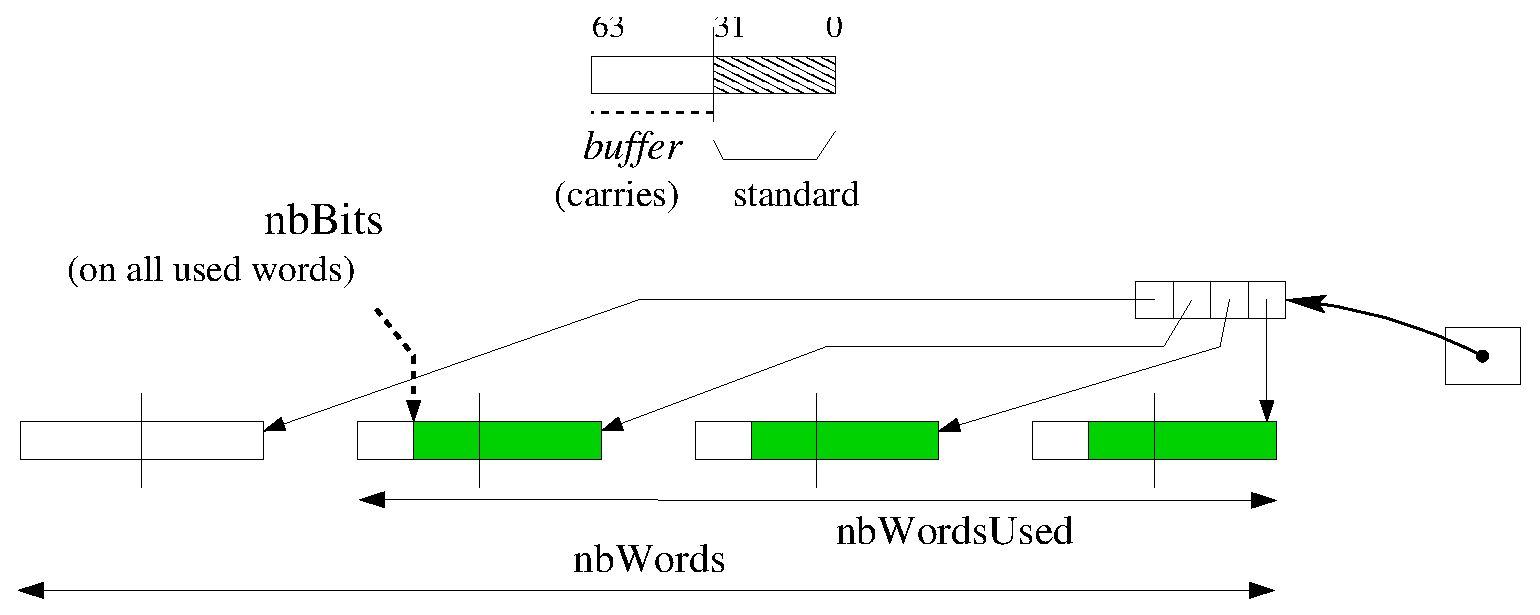
\includegraphics[scale=.5]{\locpath/figures/langford/lgf_grands_entiers}
\caption{Big integer representation, 64 bits words}
\label{fig:big-integer}
\end{figure}


\subsubsection{Gray sequence in memory: }
The Gray sequence cannot be stored in an array because it would be too large (it would contain $2^{2n}$ byte values). This is the reason why only one part of the Gray code sequence is stored in memory and the missing terms are directly computed from the known ones using arithmetic considerations.
The size of the stored part of the Gray code sequence is chosen to be as large as possible to be contained in the processor's cache memory, the L1 cache for the GPUs threads: so the accesses are fastened and the computation of the Gray code is optimized.
For an efficient use of the E5-2650 v2 ROMEO's CPUs, which disposes of 20 MB of level-3 cache, the CPU Gray code sequence is developed recursively up to depth 25. For the K20Xm ROMEO's GPUs, which dispose of 8 KB of constant memory, the sequence is developed up to depth 15. The rest of the memory is used for the computation itself. 
%As the Gray sequence is not entirely stored in memory, 
%As we show, all the gray sequence is not in memory, in order to compute the next value when the array is exceeded a modulus method is used for recompute the next value.

\subsubsection{Tasks generation and computation: }
\label{sec:tasks}

In order to perform the computation of the polynomial, two variables can be set among the $2n$ available. For the tasks generation we choose a number $p$ of variables to generate $2^p$ tasks by developing the evaluation tree to depth $p$.\\
 
 
The tasks are spread over the cluster, either synchronously or asynchronously.

\paragraph{Synchronous computation: }
A first experiment was carried out with an MPI distribution of the tasks of the previous model. 
Each MPI process finds its tasks list based on its process \textit{id}; then converting each task number into binary gives the task's initialization. 
The processes work independently; finally the root process ($id=0$) gathers all the computed numbers of solutions and sums them.

\paragraph{Asynchronous computation: }
\label{section:asynchronous}
In this case the tasks can be computed independently. 
As with the synchronous computation, the tasks' initializations are retrieved from their number. 
Each machine can get a task,  compute it, and then store its result; then when all the tasks have been computed, the partial sums are added together and the total result is provided. 

%In this case if a task is cancel due to machine error or another problem, it can be restart without compromising the end of execution.

%\subsubsection{Efficient computation}
%The computation of any task can be summarized in the four following steps:
%\begin{itemize}
%\item First it is necessary to initialize the task: with depth level $p$, $X_1=X_2=1$ and the next $p$ variables are assigned to $1$ or $-1$ depending on the task's id. The following ones are set to $1$ for example.
%\item Secondly it is necessary to set the value of each $S_i$ with the sum of $X_kX_{k + i + 1}$.
%\item Then CPU and GPU, concurrently working, go through all of the Gray sequence on the remaining $2n-p-2$ variables, by updating the $S_i$ and sum their product at each step.
%\item Finally the CPU cores computed results are summed over a shared variable; the GPU sub-tasks results are copied back and then summed with the global result.
%\end{itemize}

\subsection{Experimental settings}
This part presents the experimental context and methodology, and the way the experiments were carried out.
This study has similar goals as for the Miller's resolution experiments.

\subsubsection{Experimental methodology: }
We present here the way the experimental settings were chosen.
Firstly we define the tasks distribution, secondly we set the number of threads per GPU block; finally, we set the CPU/GPU distribution.

\paragraph{Tasks distribution depth: }
This value being set it is important to get a high number of blocks to maintain sufficient GPU load.
Thus we have to determine the best number of tasks for the distribution. As presented in part \ref{sec:tasks} the number $p$ of bits determines $2^p$ tasks. On the one hand, too many tasks are a limitation for the GPU that cannot store all the tasks in its 6GB memory. On the other hand, not enough tasks means longer tasks and too few blocks to fill the GPU grid. figure~\ref{fig:graphe_prof} shows that for the $L(2,23)$ instance the best task number is with generation depth 28.

\paragraph{Number of threads per block: }
In order to take advantage of the GPU computation power, we have to determine the threads/block distribution. Inspired by our experiments with Miller's algorithm we know that the best value may appear at lower occupancy. We perform tests on a given tasks set varying the threads/block number and grid size associated. 
Figure~\ref{fig:graphe_threads} presents the tests performed on the $n=20$ problem: the best distribution is around $128$ threads per block. 
\begin{figure}[t!]
\centering 
\includegraphics[scale=.55]{\locpath/figures/langford/graphe_threads}
\caption{$L(2,20)$, number of threads per block}
\label{fig:graphe_threads}
\end{figure}

\begin{figure}[t!]
\begin{subfigure}[b]{0.5\linewidth}
\centering 
\includegraphics[scale=.5]{\locpath/figures/langford/graphe_prof}
\caption{Influence on server generation depth}
\label{fig:graphe_prof}
\end{subfigure}
\begin{subfigure}[b]{0.5\linewidth}
\centering
\includegraphics[scale=.5]{\locpath/figures/langford/graphe_cpu_gpu}
\caption{Influence of tasks repartition}
\label{fig:graphe_rep}
\end{subfigure}
\caption{Influences of repartitions of depths and CPU-GPU tasks}
\end{figure}

\subsubsection{CPU vs GPU distribution: }
The GPU and CPU computation algorithm will approximately be the same. 
In order to take advantage of all the computational power of both components we have to balance tasks between CPU and GPU. 
We performed tests by changing the CPU/GPU distribution based on simulations on a chosen set of tasks.  
Figure~\ref{fig:graphe_rep} shows that the best distribution is obtained when the GPU handles 65\% of the tasks. 
This optimal load repartition directly results from the intrinsics computational power of each component; this repartition should be adapted if using a more powerful GPU like Tesla K40 or K80.

\subsubsection{Computing context: }

As presented in part~\ref{sec:part1_ROMEO}, we used the ROMEO supercomputer to perform our tests and computations.
%We use the same supercomputer to perform that computation that we use for the Miller method (section \ref{sec:context}), the ROMEO cluster which use Slurm as node reservation software.
On this supercomputer SLURM\cite{slurm} is used as a reservation and job queue manager.
This software allows two reservation modes: a static one-job limited reservation or the opportunity to dynamically submit several jobs in a Best-Effort manner.

\paragraph{Static distribution: }
In this case we used the synchronous distribution presented in \ref{section:asynchronous}. 
We submited a reservation with the number of MPI processes and the number of cores per process.
This method is useful to get the results quickly if we can get at once a large amount of computation resources. It was used to perform the computation of small problems, and even for $L(2,23)$ and $L(2,24)$.\\
As an issue, it has to be noted that it is difficult to quickly obtain a very large reservation on such a shared cluster, since many projects are currently running. 

\paragraph{Best effort: }
SLURM allows to submit tasks in the specific Best-Effort queue, which does not count in the user \textit{fair-share}. In this queue, if a node is free and nobody is using it, the reservation is set for a job in the best effort queue for a minimum time reservation. 
If another user asks for a reservation and requests this node, the best effort job is killed (with, for example, a SIGTERM signal). This method, based on asynchronous computation, enables a maximal use of the computational resources without blocking for a long time the entire cluster.
%This global computation process is fault-tolerant since no result is provided for aborted tasks, that are computed again.

For $L(2,27)$ and even more for $L(2,28)$ the total time required is too important to use the whole machine off a challenge period, thus we chose to compute in a Best-Effort manner.
In order to fit with this submission method we chose a reasonable time-per-task, sufficient to optimize the treatments with low loading overhead, but not too long so that killed tasks are not too penalizing for the global computation time. We empirically chose to run 15-20 minute tasks and thus we considered $p=15$ for $n=27$ and $p=17$ for $n=28$. 

The best effort based algorithm is presented on figure~\ref{fig:graphe_besteffort}.
The task handler maintains a maximum of 256 tasks in the queue; in addition the entire process is designed to be fault-tolerant since killed tasks have to be launched again.
When finished, the tasks generate an output containing the number of solutions and computation time, that is stored as a file or database entry. 
At the end the outputs of the different tasks are merged and the global result can be provided.  

\begin{figure}[t!]
\centering
\includegraphics[scale=.6]{\locpath/figures/langford/best_effort}
\caption{Best-effort distribution}
\label{fig:graphe_besteffort}
\end{figure}

%\begin{algorithm}[htbp]
%\caption{Server distribution}
%\begin{algorithmic} 
%\STATE \textbf{Variables :}
%\STATE $TQ$: tasks queue, task = integer
%\STATE $FQ$: finished tasks queue, task = integer
%\STATE $BEQ$: number of elements in the Best-Effort queue
%\STATE $N$: number of tasks
%\STATE $result$: final result
%\STATE $nbMachines$: Best-Effort queue jobs limitation
%\STATE 
%\STATE \textbf{Begin}
%\STATE $TQ\leftarrow$generate\_tasks($N$)
%\WHILE{$\#FQ \neq N$}
%\IF{$BEQ < nbMachines$}
%\STATE Start($TQ.next$)
%\ENDIF
%\ENDWHILE
%\STATE $result\leftarrow$sum($FQ$)
%\STATE \textbf{End}
%\end{algorithmic}
%\label{algo:server}
%\end{algorithm}
%
%\begin{algorithm}[htbp]
%\caption{Client task handling}
%\begin{algorithmic}
%\STATE \textbf{Variables :}
%\STATE $TQ$: tasks queue, task = integer
%\STATE $FQ$: finished tasks queue, task = integer
%\STATE $n$: number of this task
%\STATE 
%\STATE \textbf{Signal handler :}
%\IF{$SIGKILL$}
%\STATE put $n$ in the $TQ$
%\ENDIF
%\STATE 
%\STATE \textbf{Begin}
%\STATE $solution\leftarrow$compute($N$)
%\IF{$Error$}
%\STATE put $n$ in $TQ$
%\ELSE
%\STATE put $solution$ in $FQ$
%\ENDIF
%\STATE \textbf{End}
%\end{algorithmic}
%\label{algo:client}
%\end{algorithm}

\subsection{Results}
After these optimizations and implementation tuning steps, we conducted tests on the ROMEO supercomputer using best-effort queue to solve $L(2,27)$ and $L(2,28)$. 
We started the experiment after an update of the supercomputer, that implied a cluster shutdown. 
Then the machine was restarted and was about 50\% idle for the duration of our challenge. 
The computation lasted less than 2 days for $L(2,27)$ and 23 days for $L(2,28)$. 
The following describes performances considerations.

\textbf{Computing effort -} 
For $L(2,27)$, the effective computation time of the 32,768 tasks was about 30 million seconds (345.4 days), and 165,000" elapsed time (1.9 days); the average time of the tasks was 911", with a standard deviation of 20\%.
For the $L(2,28)$ 131,072 tasks the total computation time was about 1365 days (117 million seconds), as 23 day elapsed time; the tasks lasted 1321" on average with a 12\% standard deviation.

\textbf{Best-effort overhead -} 
With $L(2,27)$ we used a specific database to maintain information concerning the tasks: 617 tasks were aborted [by regular user jobs] before finishing (1.9\%), with an average computing time of 766" (43\% of the maximum requested time for a task). This consumed 472873", which overhead represents 1.6\% of the effective computing effort.

\textbf{Cluster occupancy -}
Figure~\ref{fig:graphe_15minutes_27} presents the tasks resolution over the two computation days for $L(2,27)$.
The experiment elapse time was 164700" (1.9 days). Compared to the effective computation time, we used an average of 181.2 machines (CPU-GPU couples): this represents 69.7\% of the entire cluster.
 
Figure~\ref{fig:graphe_15minutes_28} presents the tasks resolution flow during the 23 days computation for $L(2,28)$. We used about 99 machines, which represents 38\% of the 230 available nodes.

\begin{figure}[t!]
\begin{subfigure}[b]{0.5\linewidth}
\centering
\includegraphics[scale=.6]{\locpath/figures/langford/graphe_15minutes_petit}
\caption{$L(2,27)$ tasks grouped by 15" slots}
\label{fig:graphe_15minutes_27}
\end{subfigure}
\begin{subfigure}[b]{0.5\linewidth}
\centering
\includegraphics[scale=.6]{\locpath/figures/langford/graphe_15minutes_petit_28}
\caption{$L(2,28)$ tasks grouped by 1 hour slots}
\label{fig:graphe_15minutes_28}
\end{subfigure}
\caption{Task repartition for $L(2,27)$ and $L(2,28)$ }
\end{figure}

For $L(2,27)$, these results confirm that the computation took great advantage of the low occupancy of the cluster during the experiment. 
This allowed us to obtain a weak best-effort overhead, and an important cluster occupancy. 
Unfortunately for $L(2,28)$ on such a long period we got a lower part of the supercomputer dedicated to our computational project.
Thus we are confident in good perspectives for the $L(2,31)$ instance if computed on an even larger cluster or several distributed clusters. 

\section{Conclusion}

This study presents two methods to solve the Langford pairing problem on multi-GPU clusters. 
In its first part the Miller's algorithm is presented. 
Then to break the problem limitations we show optimizations and implementation of Godfrey's algorithm.

\subsection{CSP resolution method}
As any combinatorial problem can be represented as a CSP, the Miller algorithm can be seen as general resolution scheme based on the backtrack tree browsing. 
A three-level tasks generation allows to fit the multiGPU architecture. 
MPI or Best-Effort are used to spread tasks over the cluster, OpenMP for the CPU cores distribution and then CUDA to take advantage of the GPU computation power.
We were able to compute $L(2,20)$ with this regularized method and to get an even better time with the basic backtrack. 
This proves the proposed approach and also exhibits that the GPU scheduler is very efficient at managing highly divergent threads.

\subsection{MultiGPU clusters and best-effort}
In addition and with the aim to beat the Langford limit we present a new implementation of the Godfrey method using GPUs as accelerators. 
In order to use the supercomputer ROMEO, which is shared by a large scientific community, we have implemented a distribution that does not affect the machine load, using a best-effort queue. The computation is fault-tolerant and totally asynchronous.

\paragraph{Langford problem results: }
This study enabled us to compute $L(2,27)$ and $L(2,28)$ in respectively less than 2 days and 23 days on the University of Reims ROMEO supercomputer. 
The total number of solutions is: 

\hspace{3cm} L(2,27) = 111,683,611,098,764,903,232

\hspace{3cm} L(2,28) = 1,607,383,260,609,382,393,152

\paragraph{GPU benefit: }
This study shows the benefit of using GPUs as accelerators for combinatorial problems. 
In Miller's algorithm they handle 80\% of the computation effort and 65\% in Godfrey's.\\
As a near-term prospect, we want to scale and show that it is possible to use the order of 1000 or more GPUs for pure combinatorial problems.\\
The next step of this work is to generalize the method to optimization problems. 
This adds an order of complexity since shared information has to be maintained over a multiGPU cluster. 

We can conclude that even on irregular problems accelerators like GPU can be use and show better results than classical processors. 
 


%%%%%%%%%%%%%%%%%%%%%%%%%%%%%%%%%%%%%%%%%%%%%%%%%%%%%%%%%%%%%%%%%%%%%
%                                                                   %
% CHAPTER ONE, Communication WALL                                   % 
%                                                                   %
%%%%%%%%%%%%%%%%%%%%%%%%%%%%%%%%%%%%%%%%%%%%%%%%%%%%%%%%%%%%%%%%%%%%%

\documentclass[11pt,a4paper]{book}
\usepackage[utf8]{inputenc}
\usepackage[english]{babel}
\usepackage{amsmath}
\usepackage{amsfonts}
\usepackage{amssymb}
\usepackage{graphicx}
\usepackage{url}
\usepackage{python}
\usepackage{algpseudocode,algorithm}
\usepackage{tikz}
%\usepackage{todonotes}
\usepackage{makeidx}
\usepackage{enumitem}
\usepackage{array}
\usepackage{makecell}
\usepackage{xcolor}
\usetikzlibrary{positioning}
\usetikzlibrary{decorations.pathreplacing}
\usetikzlibrary{patterns}


\newcommand\todo[1]{\textcolor{red}{#1}}
\newcommand{\locpath}{../..}

\usepackage[left=2.5cm,right=2.5cm,top=2cm,bottom=2.5cm]{geometry}

% Thesis title
%\title{Energy Efficiency, Exascale and Complex Systems}
\title{Vers l'Exascale: Des Probl\`emes Th\'eoriques aux Probl\`emes Appliqu\'es\\
The Way to Exascale: From Theorics to Applied Problems}
% Author
\author{Julien Loiseau}
% Date 
\date{\today}

\makeindex

\begin{document}
\setcounter{chapter}{2}

\documentclass[11pt,a4paper]{book}
\usepackage[utf8]{inputenc}
\usepackage[english]{babel}
\usepackage{amsmath}
\usepackage{amsfonts}
\usepackage{amssymb}
\usepackage{graphicx}
\usepackage{url}
\usepackage{python}
\usepackage{algpseudocode,algorithm}
\usepackage{tikz}
%\usepackage{todonotes}
\usepackage{makeidx}
\usepackage{enumitem}
\usepackage{array}
\usepackage{makecell}
\usepackage{xcolor}
\usetikzlibrary{positioning}
\usetikzlibrary{decorations.pathreplacing}
\usetikzlibrary{patterns}


\newcommand\todo[1]{\textcolor{red}{#1}}
\newcommand{\locpath}{../..}

\usepackage[left=2.5cm,right=2.5cm,top=2cm,bottom=2.5cm]{geometry}

% Thesis title
%\title{Energy Efficiency, Exascale and Complex Systems}
\title{Vers l'Exascale: Des Probl\`emes Th\'eoriques aux Probl\`emes Appliqu\'es\\
The Way to Exascale: From Theorics to Applied Problems}
% Author
\author{Julien Loiseau}
% Date 
\date{\today}

\makeindex

\begin{document}
\setcounter{chapter}{2}

\input{\locpath/chapters/part1/chap3}

\bibliographystyle{alpha}
\bibliography{\locpath/biblio/biblio_langford,\locpath/biblio/biblio_graph,\locpath/biblio/biblio_sph,\locpath/biblio/biblio_hpc}

\end{document}


\bibliographystyle{alpha}
\bibliography{\locpath/biblio/biblio_langford,\locpath/biblio/biblio_graph,\locpath/biblio/biblio_sph,\locpath/biblio/biblio_hpc}

\end{document}


\chapter*{Conclusion}
In this part we show the real advantage of accelerators toward classical processor utilization. 
In the two exemples presented in this chapter we confronted the GPU to worst behaviors for many-core architectures: irregular applications. 
In the first one, with the problem of Langford, we worked on an irregular and computationally heavy application that does not requires much communications. 
The second one, the Graph500 BFS, was based on irregular communication over irregular memory usage. 
IN both cases we showed better results using GPU compared to classical multi-core processors. 

\subsection{Computational wall}
We studies the Langford problem under two methods of resolution. 
In the first one, the Miller algorithm, the resolution was based on a tree traversal. 
We showed that even using the irregular algorithm directly on the GPU gave us way better results than on multi-core processors. 
We showed an acceleration of quad times using the GPUs with the backtrack method.

For the second method, the Godfrey algorithm, we presented it to show how we used the GPU in order to beat a new speed record for the last instances $L(2,27)$ and $L(2,28)$.
We used the whole ROMEO supercomputer and were able to recompute them in 23 using best-effort on the cluster, a mean of 38\% of the machine.
This result can be theoretically reduce to 10 days by using the whole cluster in the same time:
 using a linear scaling which is not accurate because augmenting the number of node does not impact communications and will just allow the code to have less registers used. 

\subsection{Communication wall}
Several aspect of the Graph500 BFS makes it a good benchmark. 
The graph generated is completely random and we cannot know in advance the exact number of edges and thus the perfect behavior for distribute the data. 
During the search of the BFS algorithm the memory is completely traversed with an irregular behavior due to the random generation of the graph. 

In order to get performances we imposed regularization over our data.
The Compressed Sparse Row and Compressed Sparse Column compression methods were used and the communications were based on bitmap transfers. 

We showed that despite of the irregularity downside we were able to provide an efficient GPU algorithm, faster that the CPU algorithm and the reference code from Graph500 itself.
We provided an acceleration of two times using our CPU algorithm and quad times using our GPU algorithm.\\


From this first study, on both applications, we shows that the 
The question that arise is now: what will be the behavior of GPUs confronted to both of those aspect ? 
In order to answer this question we present in the next part the Smoothed Particle Hydrodynamics problem on which we base the last part of this study. 
We show that GPUs can also be use in this context, targeting domain scientists codes.
% Chapter Three 
\part{Application}

\chapter*{Introduction}
The first part of the thesis presented the tools needed to understand and target performances in HPC. 
The second part exposed our metric showing the benefit of accelerators, in this case GPUs, over classical processors in two contexts: irregular computation and irregular communication/memory behaviors.
We showed that the accelerators gave a real advantage on those two problems and even allows us to push the limits of performances.
We are confident that hybrid architectures will be the way to reach exascale in 2020 horizon.

In order to validate our previous results and our metric we decided to target another irregular behavior problem embedding both computation and communication/memory wall over an irregular behavior. 
This problem can also be considered as a \textit{realistic}, \textit{production} code as it targets nowadays problems of domain scientists. 
In order to show how accelerators handle real world problems, we searched for an application fulfilling our needs. 
Our choose fell on the Smoothed Particle Hydrodynamics problem applied to fluid and astrophysics simulation. 

We targeted this problem for several reasons. 
We show in the first chapter the computer science implementation issues and limitations.
We present the elements making this application a perfect choice for our metric.
This project is also part of an exchange with the Los Alamos National Laboratory in New Mexico, USA. 
This laboratory is part of the US Department of Energy, DoE, and groups thousands of researchers working on the most advanced nowadays problems.
The Los Alamos National Laboratory, LANL, is also one of the three nuclear research facilities of the US National Nuclear Security Administration (NNSA). 
In summer 2016, I made a first internship of 3 months for a summer school called: \textit{Co-Design Summer School}.
This allowed us to discover a particular class of problems, Smoothed Particle Hydrodynamics and exchange with computer scientists and domain scientists.
We extrapolate after the internship and saw what this problem really means in production context and its utility for our study. 
It makes a perfect example of realistic problem confronting computation and communication wall with irregular behavior. 
In order to characterize what physicists requested for this problem we also had another internship with the LANL in summer 2017 during three months. 

In this part we first present the Smoothed Particle Hydrodynamics method from a physical point of view and drawing a parallel with the computer science problems involved. 
Indeed, a huge amount of time have been spend on the understanding of the physics side to be able to do realistic simulations and thus realistic behavior. 
The second chapter presents a distributed SPH code working for multi-CPU and multi-GPU. 
This program is called FleCSPH. 
Starting from the framework which is the base of FleCSPH, FleCSI, we introduce the algorithm and methods to solve efficiently this problem on classical processor and the acceleration generated adding GPUs. 

%%%%%%%%%%%%%%%%%%%%%%%%%%%%%%%%%%%%%%%%%%%%%%%%%%%%%%%%%%%%%%%%%%%%%
%                                                                   %
%	CHAPTER ONE, CHOICES AND SPH                                    %
%                                                                   %
%%%%%%%%%%%%%%%%%%%%%%%%%%%%%%%%%%%%%%%%%%%%%%%%%%%%%%%%%%%%%%%%%%%%%
%%%%%%%%%%%%%%%%%%%%%%%%%%%%%%%%%%%%%%%%%%%%%%%%%%%%%%%%%%%%%%%%%%%%%
%                                                                   %
%	CHAPTER ONE, CHOICES AND SPH                                    %
%                                                                   %
%%%%%%%%%%%%%%%%%%%%%%%%%%%%%%%%%%%%%%%%%%%%%%%%%%%%%%%%%%%%%%%%%%%%%
\chapter{General problem}

\section{Introduction}
In this section we give details on our choices for the generic application confronted to both computation and communication walls on irregular context. 
This problem, Smoothed Particle Hydrodynamics, is described on the physics aspect and the difficulties involved in the resolution on supercomputers.  

\section{Combining irregular behaviors}


\section{Smoothed Particle Hydrodynamics}

\subsection{General description}
Smoothed Particle Hydrodynamics (SPH) is an explicit numerical mesh-free Lagrangian method used to solve hydrodynamical partial differential equations (PDEs) by discretized it into a set of fluid elements called particles. 
This computational method was invented for the purpose of astrophysics simulations by Monaghan, Gingold and Lucy in 1977 \cite{lucy1977numerical,gingold1977smoothed}. 
This first SPH work conserved mass and they later proposed a method which also conserves linear and angular moment \cite{gingold1982kernel}. 
The method was extended for general fluid simulation and many more fields from ballistics to oceanography. 
The development of new reliable, parallel and distributed tools for this method is a challenge for future HPC architectures with the upcoming Exascale systems.

\begin{figure}
\centering
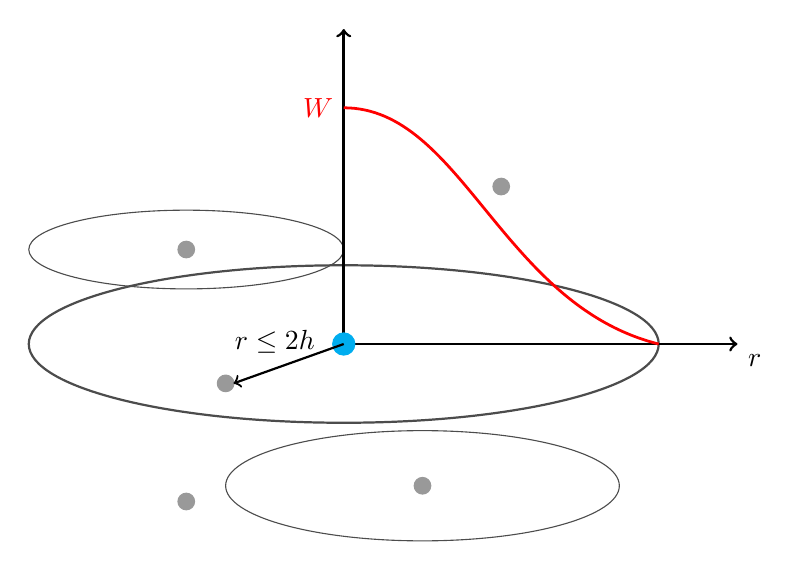
\begin{tikzpicture}
	
	% Others and their ellipse
	\draw [fill,black!40] (.5,1.5) circle (.3em);
	\draw [fill,black!40] (0,0) circle (.3em);
	\draw [fill,black!40] (0,3.2) circle (.3em);
	\draw[black!70] (0,3.2) ellipse (2 and .5);
	\draw [fill,black!40] (3,.2) circle (.3em);
	\draw[black!70] (3,.2) ellipse (2.5 and .7);
	\draw [fill,black!40] (4,4) circle (.3em);
	% Ellipses 
	\draw[line width=.8pt,black!70] (2,2) ellipse (4 and 1);
	% Axes
	\draw[->,line width=1pt] (2,2) -- (7,2) node[anchor=north west] {$r$};
	\draw[->,line width=1pt] (2,2) -- (2,6);
	% bezier for kernel 
	\draw[red,line width=1pt]  (6,2) .. controls (4,2.5) and (3.5,5) .. (2,5) node[red,anchor=east] {$W$};
	% main particle, at the end to cover
	\draw [fill,cyan] (2,2) circle (.4em);
	% Arrows 
	\draw[->,line width=.8pt] (2,2) -- (.6,1.5) node[midway, above,xshift=-.5em] {$r\leq2h$};
\end{tikzpicture}
%\includegraphics[scale=.4]{\locpath/figures/flecsph/sph.pdf}
\caption{SPH kernel $W$ and smoothing length $h$ representation}
\label{fig:sph_base}
\end{figure}

The method, as illustrated in Fig.~\ref{fig:sph_base}, computes the evolution of physical quantities for every particle regarding its neighbors in the radius of its smoothing length $h$. 
The particles in this radius are then valued according to their distance using a smoothing function $W$, also called a kernel. 
The fundamental SPH formulation for any physical quantity $A$ is then to compute with all the neighbors of $b$ of a particle by:
\begin{equation}
A(\vec{r}) \simeq \sum_b \frac{m_b}{\rho_b} A(\vec{r}_b) W ( |\vec{r}-\vec{r}_b|,h)
\end{equation}

On a physics aspect, this method has several advantages:
It can handle deformations, low densities, vacuum, and makes particle tracking easier. 
It also conserves mass, linear and angular momenta, and energy by its construction that implies independence of the numerical resolution. 
Another strong benefit of using SPH is its exact advection of fluid properties. 
Furthermore, the particle structure of SPH easily combines with tree methods for solving Newtonian gravity through N-body simulations.
As a mesh-free method, it avoids the need of grid to calculate the spatial derivatives. 

However, there are cons to consider using SPH: 
It is restricted to low-order rate of convergence on certain PDE formulations; 
It requires careful setup of initial distribution of particles; 
Further, it can be struggle to resolve turbulence-dominated flows and special care must be taken when handling high gradients such as shocks and surface structure of neutron stars.
Many works are leading to handle more cases and to push the limitations of this method \cite{dai2017dual,lind2016incompressible,ren2016dual}.

In this work, we are solving Lagrangian conservation equations (Euler equations) for mass, energy and momentum of an ideal fluid ~\cite{Landau1959}  such that:
\begin{equation}
\frac{d \rho}{d t} = - \rho \nabla \cdot \vec{v}, \quad
\frac{d u}{d t} = \left( \frac{P}{\rho^2} \right) \frac{d \rho}{d t}, \quad
\frac{d \vec{v}}{d t} = - \frac{\nabla P}{\rho}
\end{equation}
with $\rho$ the density, $P$ the pressure, $u$ the internal energy and $v$ the velocity, where $d/dt = \partial_t + \vec{v} \cdot \nabla$ which is convective derivative.

By using the volume element $V_b = m_b / \rho_b$, we can formulate the Newtonian SPH scheme~\cite{rosswog2009} such that
\begin{equation}
\label{eq:rho}
\rho_a = \sum_b m_b W_{ab} (h_a)
\end{equation}
\begin{equation}
\frac{d u_a}{dt} = \frac{P_a}{\rho_a^2} \sum_b m_b \vec{v}_{ab} \cdot \nabla_a W_{ab} 
\end{equation}
\begin{equation}
\frac{d \vec{v}_a}{d t} = - \sum_b m_b \left(\frac{P_a}{\rho_a^2} + \frac{P_b}{\rho_b^2} \right) \nabla_a W_{ab}
\end{equation}
where $W_{ab} = W(| \vec{r}_a - \vec{r}_b |,h)$ is the smoothing kernel. 
The equations we would like to solve allow for emergence of discontinuities from smooth initial data. 
At discontinuities, the entropy increases in shocks. That dissipation occurs inside the shock-front. 
The SPH formulation here is inviscid so we need to handle this dissipation near shocks. 
There are a number of way to handle this problem, but the most widespread approach is to add artificial viscosity (or artificial dissipation) terms in SPH formulation such that:
\begin{equation}
\left(\frac{d u_a}{dt} \right)_{art} = \frac{1}{2} \sum_b m_b \Pi_{ab} \vec{v}_{ab} \cdot \nabla_a W_{ab}
\end{equation}
\begin{equation}
\left(\frac{d\vec{v}_a}{dt} \right)_{art} = - \sum_b m_b \Pi_{ab}\nabla_a W_{ab}
\end{equation}
In general, we can express the equations for internal energy and acceleration with artificial viscosity
\begin{equation}
\label{eq:intern}
\frac{d u_a}{dt} = \sum_b m_b \left(\frac{P_a}{\rho_a^2} + \frac{\Pi_{ab}}{2} \right) \vec{v}_{ab} \cdot \nabla_a W_{ab}
\end{equation}
\begin{equation}
\label{eq:velo}
\frac{d \vec{v}_a}{d t} = - \sum_b m_b \left(\frac{P_a}{\rho_a^2} + \frac{P_b}{\rho_b^2} + \Pi_{ab} \right) \nabla_a W_{ab}
\end{equation}
$\Pi_{ab}$ is the artificial viscosity tensor. 
As long as $\Pi_{ab}$ is symmetric, the conservation of energy, linear and angular momentum is assured by the form of the equation and antisymmetry of the gradient of kernel with respect to the exchange of indices $a$ and $b$. $\Pi_{ab}$ may define different way but here we use~\cite{Monaghan1983} such as: 
\begin{equation}
\Pi_{ab} = \begin{cases}
\frac{- \alpha \bar{c}_{ab} \mu_{ab} + \beta \mu_{ab}^2}{\bar{\rho}_{ab}} & \text{for $\vec{r}_{ab} \cdot \vec{v}_{ab} < 0$} \\
0 & \text{otherwise}
\end{cases}
\end{equation}
\begin{equation}
\mu_{ab} = \frac{\bar{h}_{ab} \vec{r}_{ab} \cdot \vec{v}_{ab}}{r^2_{ab} + \epsilon \bar{h}_{ab}^2}
\end{equation}

Using the usual form $c_s$ as $c_s = \sqrt{\frac{\partial p}{\partial \rho}}$.
The values of $\epsilon$, $\alpha$, and $\beta$ have to be set regarding the problem targeted. 
Here, we use $\epsilon = 0.01h^2$, $\alpha = 1.0$, and $\beta = 2.0$. 

There are many possibilities for the smoothing function, called the kernel. 
As an example the Monaghan's cubic spline kernel is given by:
\begin{equation}
W(\vec{r},h) = \frac{\sigma}{h^D} \begin{cases}
1-\frac{3}{2} q^2 + \frac{3}{4} & \text{if} \indent 0 \leq q \leq 1 \\
\frac{1}{4} (1-q)^3  & \text{if} \indent 1 \leq q \leq 2 \\
0 & \text{otherwise}
\end{cases}
\end{equation}
where $q = r/h$, $r$ the distance between the two particles, $D$ is the number of dimensions and $\sigma$ is a normalization constant with the values:
\begin{equation}
\sigma =  \begin{cases}
\frac{2}{3} & \text{for 1D}  \\
\frac{10}{7 \pi} & \text{for 2D} \\
\frac{1}{\pi} & \text{for 3D}
\end{cases}
\end{equation}

To sum up, the SPH resolution scheme and its routines are presented on algorithm \ref{alg:sph}.
The Equation of State (EOS) and the integration are problem dependent and will be define for each test case in section \ref{sec:applications}. 

\begin{algorithm}
\caption{SPH loop algorithm}\label{alg:sph}
\begin{algorithmic}[1]
\While{not last step}
\State Compute density for each particle (\ref{eq:rho})
\State Compute pressure using EOS 
\State Compute acceleration from pressure forces (\ref{eq:velo})
\State Compute change of internal energy for acceleration (\ref{eq:intern})
\State Advance particles after integration
\EndWhile
\end{algorithmic}
\end{algorithm}

The main downside for the implementation of this method is the requirement for local computation on every particle. 
The particles have to be grouped locally to perform the computation of (\ref{eq:rho}), (\ref{eq:intern}) and (\ref{eq:velo}).
A communication step is needed before and after (\ref{eq:rho}) to get the local physical data to be able to compute (\ref{eq:intern}) and (\ref{eq:velo}).
The tree data structure allows us to perform $O(Nlog(N))$ neighbor search but also add a domain decomposition and distribution layer.

As the SPH method is used in a large panel of fields from astrophysics to fluid mechanic, there are numerous related works. 
We can cite a code developed in the LANL, 2HOT \cite{warren20132hot} that introduced the Hashed Oct Tree structure used in our implementation. 
There is also GADGET-2 \cite{springel2005cosmological}, GIZMO \cite{hopkins2014gizmo} and the most recent publication is GASOLINE \cite{wadsley2017gasoline2} based on PKDGRAV, a specific tree+gravity implementation. 
Several implementations already implement GPU code and tree construction and traversal, one can cite GOTHIC \cite{miki2017gothic}, presenting gravitational tree code accelerated using the latest Fermi, Kepler and Maxwell architectures. But a lot of GPU accelerated work still focused on fluid problems and not on astrophysical problems  \cite{harada2007smoothed,crespo2011gpus}.
We also note that these implementations focus on SPH problems and does not provide a general purpose and multi-physics framework like we intent to provide through FleCSPH and FleCSI. 

\subsection{Gravitation}
For classical problems like fluid flow the gravitation can directly be applied on the particles with the force:
\begin{equation}
	\vec{a_g} = m\vec{g}
\end{equation}

In order to consider astrophysics problems we need to introduice self-gravitation. 
Each particle imply an action on the others base on its distance and mass. 
The equation of gravitation for a particle $i$ with $j$ other particles is: 
\begin{equation}
	\vec{f_a}_i = \sum_j -G \frac{m_i m_j}{|\vec{r_i}-\vec{r_j}|^3} \vec{r_{ij}}
	\label{eq:gravitation}
\end{equation}

This computation involve an $O(N^2)$ complexity and thus is not applicable directly. 
We applied the method called Fast Multipole Method, FMM and discussed in \cite{beatson1997short}.
In this method we compute the gravitation up a approximations. 
The user can refine those approximation changing parameters. 

\begin{figure}
\resizebox {\columnwidth} {!} {
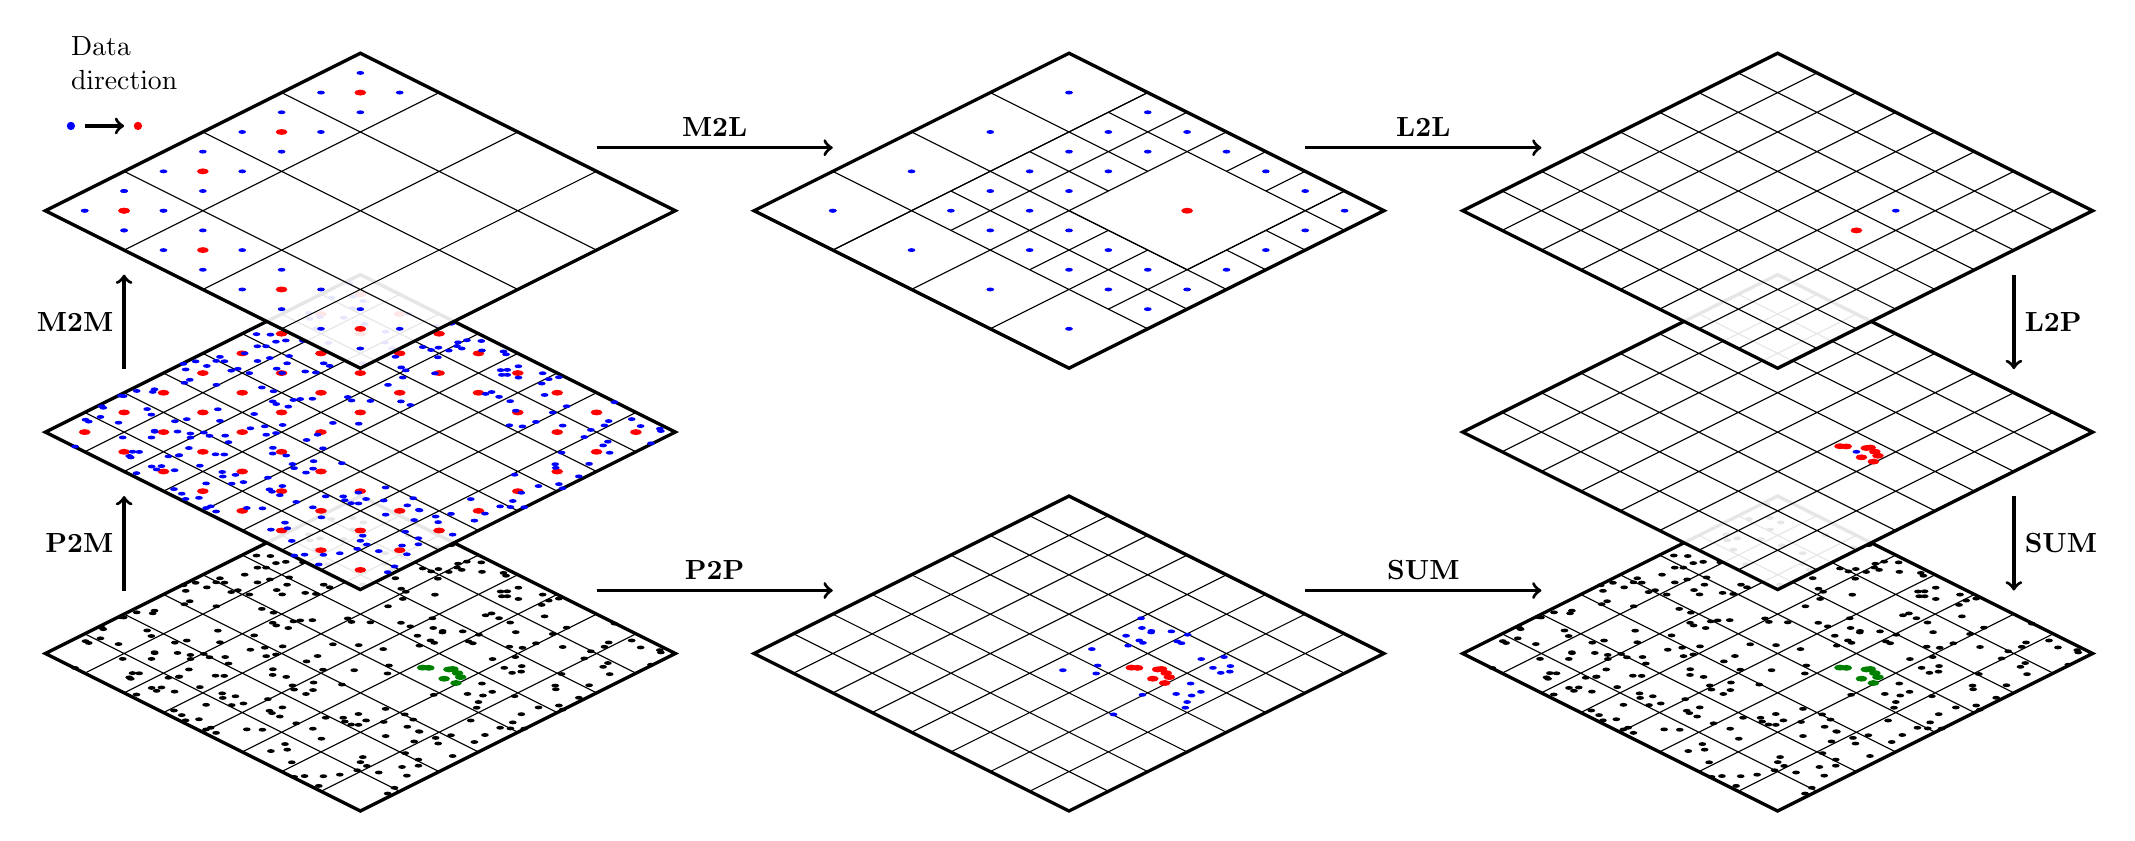
\begin{tikzpicture}
\def\nrand{300}
\def\seed{12}
\def\gridSize{5mm}
\def\gridTotal{4}
% Particles to Multipole
\pgfmathsetseed{\seed}
\begin{scope}[
   		yshift=0,every node/.append style={
    		yslant=0.5,xslant=-1},yslant=0.5,xslant=-1
    ]
    \fill[white,fill opacity=.9] (0,0) rectangle (4,4);
    \draw[black,very thick] (0,0) rectangle (4,4);
	\draw[step=\gridSize, black] (0,0) grid (\gridTotal,\gridTotal);
	\foreach \i in {1,2,...,\nrand}{
    	\pgfmathsetmacro{\x}{(rand)*2+2}
    	\pgfmathsetmacro{\y}{(rand)*2+2}
		% COLOR 
		\ifthenelse{\( \lengthtest{\x cm>2cm} \AND \lengthtest{\x cm<2.5cm} \)}
		{	
			\ifthenelse{ \( \lengthtest{\y cm>1cm} \AND \lengthtest{\y cm<1.5cm} \)}
			{\node at (\x,\y) [black!50!green,circle,fill,inner sep=.7pt,minimum size=3pt]{};}
			{\node at (\x,\y) [circle,fill,inner sep=.7pt]{};}
		}
		{\node at (\x,\y) [circle,fill,inner sep=.7pt]{};}
	}
\end{scope}
\pgfmathsetseed{\seed}
\begin{scope}[
   		yshift=80,every node/.append style={
    		yslant=0.5,xslant=-1},yslant=0.5,xslant=-1
    ]
    \fill[white,fill opacity=.9] (0,0) rectangle (4,4);
    \draw[black,very thick] (0,0) rectangle (4,4);
	\draw[step=5mm, black] (0,0) grid (\gridTotal,\gridTotal);
	\foreach \x in {0,1,...,7}{\foreach \y in {0,1,...,7}{
		\ifthenelse{\( \x<3 \OR \x>5 \)}
		{
			\node at (\x*\gridSize+\gridSize/2,\y*\gridSize+\gridSize/2)[red,circle,fill,inner sep=.7pt,minimum size=3pt]{};
		}
		{	\ifthenelse{ \( \y<1 \OR \y>3 \)}
			{
			\node at (\x*\gridSize+\gridSize/2,\y*\gridSize+\gridSize/2)[red,circle,fill,inner sep=.7pt,minimum size=3pt]{};	
			}{}
		}
	}}
	\foreach \i in {1,2,...,\nrand}{
    	\pgfmathsetmacro{\x}{(rand)*2+2}
    	\pgfmathsetmacro{\y}{(rand)*2+2}
    	\ifthenelse{\( \lengthtest{\x cm<1.5cm} \OR \lengthtest{\x cm>3cm} \)}
		{\node at (\x,\y) [blue,circle,fill,inner sep=.7pt]{};}
		{	\ifthenelse{ \( \lengthtest{\y cm<.5cm} \OR \lengthtest{\y cm>2cm} \)}
			{\node at (\x,\y) [blue,circle,fill,inner sep=.7pt]{};}
			{}
		}
  	}
\end{scope}
\begin{scope}[
   		yshift=160,every node/.append style={
    		yslant=0.5,xslant=-1},yslant=0.5,xslant=-1
    ]
    \fill[white,fill opacity=.9] (0,0) rectangle (4,4);
    \draw[black,very thick] (0,0) rectangle (4,4);
	\draw[step=10mm, black] (0,0) grid (4,4);
	\foreach \x in {0,1}{\foreach \y in {0,...,7}{
		\node at (\x*\gridSize+\gridSize/2,\y*\gridSize+\gridSize/2)[blue,circle,fill,inner sep=.7pt]{};
	}}
	\foreach \x in {0,...,7}{\foreach \y in {6,7}{
		\node at (\x*\gridSize+\gridSize/2,\y*\gridSize+\gridSize/2)[blue,circle,fill,inner sep=.7pt]{};
	}}

	\foreach \x in {0}{\foreach \y in {0,...,3}{				  
		\node at (\x*\gridSize*2+\gridSize,\y*\gridSize*2+\gridSize) [red,circle,fill,inner sep=.7pt,minimum size=3pt]{};
	}}
	\foreach \x in {0,...,3}{\foreach \y in {3}{				  
		\node at (\x*\gridSize*2+\gridSize,\y*\gridSize*2+\gridSize) [red,circle,fill,inner sep=.7pt,minimum size=3pt]{};
	}}
\end{scope}

%PARTICLES TO PARTICLES
\pgfmathsetseed{\seed}
\begin{scope}[
   		yshift=0,xshift=9cm,every node/.append style={
    		yslant=0.5,xslant=-1},yslant=0.5,xslant=-1
    ]
    \fill[white,fill opacity=.9] (0,0) rectangle (4,4);
    \draw[black,very thick] (0,0) rectangle (4,4);
	\draw[step=5mm, black] (0,0) grid (4,4);
	\foreach \i in {1,2,...,\nrand}{
    	\pgfmathsetmacro{\x}{(rand)*2+2}
    	\pgfmathsetmacro{\y}{(rand)*2+2}
    	\ifthenelse{\( \lengthtest{\x cm>1.5cm} \AND \lengthtest{\x cm<3cm} \)}
		{	
			\ifthenelse{ \( \lengthtest{\y cm>.5cm} \AND \lengthtest{\y cm<2cm} \)}
			{
				% COLOR 
				\ifthenelse{\( \lengthtest{\x cm>2cm} \AND \lengthtest{\x cm<2.5cm} \)}
				{	
					\ifthenelse{ \( \lengthtest{\y cm>1cm} \AND \lengthtest{\y cm<1.5cm} \)}
					{\node at (\x,\y) [red,circle,fill,inner sep=.7pt,minimum size=3pt]{};}
					{\node at (\x,\y) [blue,circle,fill,inner sep=.7pt]{};}
				}
				{\node at (\x,\y) [blue,circle,fill,inner sep=.7pt]{};}
			}{}
		}{}
    	%\node at (\x,\y) [circle,fill,inner sep=.7pt]{};
  	}
\end{scope}
%MULTIPOLE TO MULTIPOLE
\begin{scope}[
   		yshift=160,xshift=9cm,every node/.append style={
    		yslant=0.5,xslant=-1},yslant=0.5,xslant=-1
    ]
    \fill[white,fill opacity=.9] (0,0) rectangle (4,4);
    \draw[black,very thick] (0,0) rectangle (4,4);
    \draw[step=10mm, black] (0,3) grid (4,4);
	\draw[step=10mm, black] (0,0) grid (1,3);
	\draw[step=5mm, black] (1,0) grid (2,3);
	\draw[step=5mm, black] (2,2) grid (4,3);
	\draw[step=5mm, black] (2,0) grid (4,.5);
	\draw[step=5mm, black] (3.5,0) grid (4,2);
	% add rectangle
	\draw[black] (2,.5) rectangle (3.5,2);
	% Big part 
	\foreach \x in {0}{\foreach \y in {0,...,3}{				  
		\node at (\x*\gridSize*2+\gridSize,\y*\gridSize*2+\gridSize) [blue,circle,fill,inner sep=.7pt]{};
	}}
	\foreach \x in {0,...,3}{\foreach \y in {3}{				  
		\node at (\x*\gridSize*2+\gridSize,\y*\gridSize*2+\gridSize) [blue,circle,fill,inner sep=.7pt]{};
	}}
	% Smaller one 
	\foreach \x in {2,3}{\foreach \y in {0,...,3}{
		\node at (\x*\gridSize+\gridSize/2,\y*\gridSize+\gridSize/2)[blue,circle,fill,inner sep=.7pt]{};
	}}

	\foreach \x in {2,...,7}{\foreach \y in {4,5}{
		\node at (\x*\gridSize+\gridSize/2,\y*\gridSize+\gridSize/2)[blue,circle,fill,inner sep=.7pt]{};
	}}

	\foreach \x in {7}{\foreach \y in {0,...,3}{
		\node at (\x*\gridSize+\gridSize/2,\y*\gridSize+\gridSize/2)[blue,circle,fill,inner sep=.7pt]{};
	}}
	\foreach \x in {4,5,6}{\foreach \y in {0}{
		\node at (\x*\gridSize+\gridSize/2,\y*\gridSize+\gridSize/2)[blue,circle,fill,inner sep=.7pt]{};
	}}
	\node at (5*\gridSize+\gridSize/2,2*\gridSize+\gridSize/2) [red,circle,fill,inner sep=.7pt,minimum size=3pt]{};
\end{scope}

% Multipole to Particles 
\pgfmathsetseed{\seed}
\begin{scope}[
   		yshift=0,xshift=18cm,every node/.append style={
    		yslant=0.5,xslant=-1},yslant=0.5,xslant=-1
    ]
    \fill[white,fill opacity=.9] (0,0) rectangle (4,4);
    \draw[black,very thick] (0,0) rectangle (4,4);
	\draw[step=5mm, black] (0,0) grid (4,4);
	\foreach \i in {1,2,...,\nrand}{
    	\pgfmathsetmacro{\x}{(rand)*2+2}
    	\pgfmathsetmacro{\y}{(rand)*2+2}
		% COLOR 
		\ifthenelse{\( \lengthtest{\x cm>2cm} \AND \lengthtest{\x cm<2.5cm} \)}
		{	
			\ifthenelse{ \( \lengthtest{\y cm>1cm} \AND \lengthtest{\y cm<1.5cm} \)}
			{\node at (\x,\y) [black!50!green,circle,fill,inner sep=.7pt,minimum size=3pt]{};}
			{\node at (\x,\y) [circle,fill,inner sep=.7pt]{};}
		}
		{\node at (\x,\y) [circle,fill,inner sep=.7pt]{};}
	}
\end{scope}
\pgfmathsetseed{\seed}
\begin{scope}[
   		yshift=80,xshift=18cm,every node/.append style={
    		yslant=0.5,xslant=-1},yslant=0.5,xslant=-1
    ]
    \fill[white,fill opacity=.9] (0,0) rectangle (4,4);
    \draw[black,very thick] (0,0) rectangle (4,4);
	\draw[step=5mm, black] (0,0) grid (4,4);

	\foreach \i in {1,2,...,\nrand}{
    	\pgfmathsetmacro{\x}{(rand)*2+2}
    	\pgfmathsetmacro{\y}{(rand)*2+2}
    	\ifthenelse{\( \lengthtest{\x cm>1.5cm} \AND \lengthtest{\x cm<3cm} \)}
		{	
			\ifthenelse{ \( \lengthtest{\y cm>.5cm} \AND \lengthtest{\y cm<2cm} \)}
			{
				% COLOR 
				\ifthenelse{\( \lengthtest{\x cm>2cm} \AND \lengthtest{\x cm<2.5cm} \)}
				{	
					\ifthenelse{ \( \lengthtest{\y cm>1cm} \AND \lengthtest{\y cm<1.5cm} \)}
					{\node at (\x,\y) [red,circle,fill,inner sep=.7pt,minimum size=3pt]{};}
					{}
				}{}
			}{}
		}{}
	}
	\node at (4*\gridSize+\gridSize/2,2*\gridSize+\gridSize/2) [blue,circle,fill,inner sep=.7pt]{};
\end{scope}
%% MULTIPOLE TO LOCAL
\begin{scope}[
   		yshift=160,xshift=18cm,every node/.append style={
    		yslant=0.5,xslant=-1},yslant=0.5,xslant=-1
    ]
    \fill[white,fill opacity=.9] (0,0) rectangle (4,4);
    \draw[black,very thick] (0,0) rectangle (4,4);
	\draw[step=5mm, black] (0,0) grid (4,4);
	\node at (4*\gridSize+\gridSize/2,2*\gridSize+\gridSize/2) [red,circle,fill,inner sep=.7pt,minimum size=3pt]{};

	\node at (5*\gridSize+\gridSize/2,2*\gridSize+\gridSize/2) [blue,circle,fill,inner sep=.7pt]{};
\end{scope}
% ARROWS AND TEXT
\draw[->,very thick] (-3,2.8) -- (-3,4) node[midway,left] {\textbf{P2M}};
\draw[->,very thick] ([yshift=80]-3,2.8) -- ([yshift=80]-3,4) node[midway,left] {\textbf{M2M}};

\draw[->,very thick] ([yshift=160]3,2.8) -- ([yshift=160]6,2.8) node[midway,above] {\textbf{M2L}};
\draw[->,very thick] ([yshift=160,xshift=9cm]3,2.8) -- ([yshift=160,xshift=9cm]6,2.8) node[midway,above] {\textbf{L2L}};

\draw[<-,very thick] ([yshift=80]21,2.8) -- ([yshift=80]21,4) node[midway,right] {\textbf{L2P}};
\draw[<-,very thick] (21,2.8) -- (21,4) node[midway,right] {\textbf{SUM}};

\draw[->,very thick] (3,2.8) -- (6,2.8) node[midway,above] {\textbf{P2P}};
\draw[->,very thick] ([xshift=9cm]3,2.8) -- ([xshift=9cm]6,2.8) node[midway,above] {\textbf{SUM}};


\draw[->,very thick] (-3.5,8.7cm) node[xshift=-5pt,blue,circle,fill,inner sep=.7pt,minimum size=3pt] (a) {} -- 
 (-3,8.7cm) node[xshift=5pt,red,circle,fill,inner sep=.7pt,minimum size=3pt] (b) {};
\node[align=left] at (-3,9.5cm) {Data\\direction};


\end{tikzpicture}
}
\caption{Fast Multipole Method schematics. Particles to Multipole (P2M), Multipole to Multipole (M2M), Multipole to Particles (M2P), Multipole to Local (M2L), Local to Local (L2L) and Particles to Particles (P2P). Schematic inspired from \cite{yokota2011treecode}}
\end{figure}

This method is based on Taylor series.
The gravitation function of equation~\ref{eq:gravitation} can be approximate on a particle at position $\vec{r}$ by the gravitation computed at the centroid at position $\vec{r_c}$: 
\begin{equation}
 \vec{f}(\vec{r}) = \vec{f}(\vec{r_c}) + ||\frac{\partial\vec{f}}{\partial\vec{r}}||\cdot (\vec{r} - \vec{r_c}) + \frac{1}{2} (\vec{r}-\vec{r_c})^\intercal \cdot   ||\frac{\partial\vec{f}}{\partial\vec{r} \partial\vec{r}}|| \cdot (\vec{r} - \vec{r_c})
 \end{equation}

 From equation~\ref{eq:gravitation} we compute the term $||\frac{\partial\vec{f}}{\partial\vec{r}}||$:s
 \begin{equation}
\frac{\partial\vec{f}}{\partial\vec{r}} =
- \sum_p \frac{m_p}{|\vec{r_c}-\vec{r_p}|^3}
\begin{bmatrix}
1 - \frac{3(x_c-x_p)(x_c-x_p)}{|\overline{r_c}-\overline{r_p}|^2} & -\frac{3(y_c-y_p)(x_c-x_p)}{|\overline{r_c}-\overline{r_p}|^2}  & -\frac{3(z_c-z_p)(x_c-x_p)}{|\vec{r_c}-\vec{r_p}|^2}  \\
-\frac{3(x_c-x_p)(y_c-y_p)}{|\vec{r_c}-\vec{r_p}|^2}  & 1 - \frac{3(y_c-y_p)(y_c-y_p)}{|\vec{r_c}-\vec{r_p}|^2} &  -\frac{3(z_c-z_p)(y_c-y_p)}{|\vec{r_c}-\vec{r_p}|^2}\\
- \frac{3(x_c-x_p)(z_c-z_p)}{|\vec{r_c}-\vec{r_p}|^2}   &  -\frac{3(y_c-y_p)(z_c-z_p)}{|\vec{r_c}-\vec{r_p}|^2} &  1- \frac{3(z_c-z_p)(z_c-z_p)}{|\vec{r_c}-\vec{r_p}|^2} \\
\end{bmatrix}
 \end{equation}

And we propose a compact version of the matrix with: 
 
\begin{equation}
 ||\frac{\partial f^a}{\partial r^b}|| = -\sum_c \frac{m_c}{|\vec{r}-\vec{r_c}|^3} \Big[ \delta_{ab} - \frac{3.(r^a-r_c^a)(r^b-r_c^b)}{|\vec{r}-\vec{r_c}|^2} \Big] 
\end{equation}

With $\delta_{ab}$ the kronecker delta:
\begin{equation}
\delta_{ab} = 
\begin{cases}
    1, & \text{if $a = b$}.\\
    0, & \text{if $a\neq b$}.
  \end{cases}
\end{equation}

We note that $a$ and $b$ variate from 0 to 2 and $r^0=x$, $r^1=y$, and $r^2=z$ as usual sense. 

For the term $||\frac{\partial\vec{f}}{\partial\vec{r} \partial\vec{r}}||$ we give the compact version by:
\begin{equation}
||\frac{\partial^2 f^a}{\partial r^b \partial r^c}|| =
- \sum_c \frac{3 m_c}{|\vec{r}-\vec{r_c}|^5} \left[\frac{5(r^a-r_c^a)(r^b-r_c^b)(r^c-r_c^c)}{|\vec{r}-\vec{r_c}|^2} - \left( \delta_{ab} (r^c-r_c^c)+\delta_{bc} (r^a-r_c^a)+\delta_{ac} (r^b-r_c^b) \right) \right] 
 \end{equation} 

 \begin{figure}
 \end{figure}

The method is summed up in figure with the different equations.
We consider Centers Of Mass, COM, to be the centroid of particles based on their position. 
In several steps the information is first transmitted to the COMs, computing their position and mass. 


\subsection{Problems} 
The previous equations are generic and describe the behavior of SPH method. 
In order to check our 

\subsubsection{Sod shock tube}

\subsubsection{Sedov blast wave}

\subsubsection{Fluid flow}

\subsubsection{Astrophysics: neutron stars coalescence}

The final aim of our tests is to simulate astrophysical events. 
We are interested in one of the most important event recently discovered. 
Last year the Laser Interferometer Gravitational Wave, LIGO, detected the first gravitational wave generated by binary neutron stars merging \cite{abbott2017gw170817} and also more complexes event with Binary Black Holes coalescence in \cite{abbott2017gw170814}.


\paragraph{Solving Lane-Emden Equation}

We need to determine the density function based on the radius. 

As we consider the star as a polytropic fluid, we use the equation of Lane-Emden which is a form of the Poisson equation: 

\begin{equation}\label{eq_LaneEmden}
  \frac{d^2\theta}{d \xi^2}+ \frac{2}{\xi}\frac{d\theta}{d\xi}+\theta^n = 0
\end{equation}

With $\xi$ and $\theta$ two dimensionless variables. 
There is only exact solutions for a polytropic index $n = 0.5$, $1$ and $2$.
In our work we use a polytropic index of $1$ which can correspond to a NS simulation.

For $n=1$ the solution of equation \ref{eq_LaneEmden} is: 

\begin{equation}
\theta(\xi)=\frac{sin(\xi)}{\xi}
\end{equation}

We note $\xi_1 = \pi$, the first value of $\xi$ as $\theta(\xi) = 0$.
$\theta(\xi)$ is also defined as: 
\begin{equation}
 \theta(\xi) = \Big(\frac{\rho(\xi)}{\rho_c}\Big)^{\frac{1}{n}}  = \frac{\rho(\xi)}{\rho_c}
\end{equation}

With $\rho_c$ the internal density of the star and $\rho$ the density at a determined radius. $\xi$ is defined as:  
$$ \xi = Ar = \sqrt{\frac{4\pi G}{K(n+1)}\rho_c^{(n-1)/n}} \times r = \sqrt{\frac{2\pi G}{K}}\times r \mbox{ (for } n=1 \mbox{)}$$

With $K$ a proportionality constant.

From the previous equations we can write the stellar radius $R$ as:
\begin{equation}
R = \sqrt{\frac{K(n+1)}{4\pi G}}\rho_c^{(1-n)/2}\xi_1 = \sqrt{ \frac{K}{2\pi G} } \times \xi_1
\end{equation} 

(We note that for $n=1$ the radius does not depend of the central density.)

If, for example, we use dimensionless units as $G=R=M=1$ (for the other results we use CGS with $G = 6.674 \times 10^{-8} cm^3g^{-1}s^{-2}$) 
We can compute K as: 
\begin{equation}
\label{eq:constant}
K = \frac{R^2  2 \pi G}{\xi_1^2}
\end{equation}

\begin{center}

\begin{tabular}{c|c|c|c|c|}
 & $NS_1$ & $NS_2$ & $NS_3$ & $NS_4$ \\ 
\hline 
Radius (cm) & $R=G=M=1$ & 1500000 & 1400000 & 960000 \\ 
\hline 
K & 0.636619 & 95598.00 & 83576.48 & 39156.94\\ 
\hline 
\end{tabular}

\end{center} 

Then we deduce the density function of $r$ as :

$$\rho(\xi) = \frac{sin(A\times r)}{A \times r} \times \rho_c \mbox{ with } A = \sqrt{\frac{2\pi G}{K}}
$$

As we know the total Mass $M$, the radius $R$ and the gravitational constant $G$ we can compute the central density as: 

$$ \rho_c = \frac{M A^3}{4 \pi (sin(AR)-ARcos(AR)) } $$

Then we normalize the results to fit $R = M = G = 1$: $K' = K/(R^2G) $, $m_i' = m_i/M $, $h_i' = h_i / R$, $\vec{x_i}' = \vec{x_i}/R$ 

\section{Conclusion}



%%%%%%%%%%%%%%%%%%%%%%%%%%%%%%%%%%%%%%%%%%%%%%%%%%%%%%%%%%%%%%%%%%%%%
%                                                                   %
%	CHAPTER TWO, FLECSPH.                                           %
%                                                                   %
%%%%%%%%%%%%%%%%%%%%%%%%%%%%%%%%%%%%%%%%%%%%%%%%%%%%%%%%%%%%%%%%%%%%%
%%%%%%%%%%%%%%%%%%%%%%%%%%%%%%%%%%%%%%%%%%%%%%%%%%%%%%%%%%%%%%%%%%%%%
%                                                                   %
% CHAPTER FIVE: COMPUTATIONAL WALL: LANGFORD PROBLEM                %
%                                                                   %
%%%%%%%%%%%%%%%%%%%%%%%%%%%%%%%%%%%%%%%%%%%%%%%%%%%%%%%%%%%%%%%%%%%%%

\chapter{Computational Wall: Langford Problem}

\section{Introduction}
Our aim is to determine the behavior of accelerators compared to classical processor in case of irregular-computationally heavy problems.
For this purpose we choose the Langford problem which is an academic problem of combinatorial counting.
We show the optimizations made to the regular processor algorithm to efficiently implement this application on GPU. 
We compare the two approaches from classical processor to GPU implementation. 
The results are then presented to show the acceleration using the whole ROMEO supercomputer.
This study shows two approaches to the Langford problem.
The Miller's algorithm, irregular tree backtracking and the the Godfrey's method which is use in order to beat a time record on this problem.\\

C. Dudley Langford gave his name to a classic permutation problem ~\cite{Gard56, Simp83}.  
While observing his son manipulating blocks of different colors, he noticed that it was possible to arrange three pairs of different colored blocks (yellow, red and blue) in such a way that only one block separates the red pair - noted as pair 1 - , two blocks separate the blue pair - noted as pair 2 - and finally three blocks separate the yellow one - noted as pair 3 - , see figure~\ref{fig:lang}.\\

\begin{figure}[htbp]    
\begin{center}    
%\includegraphics[scale=0.45]{\locpath/figures/langford/lgf_cubes}   
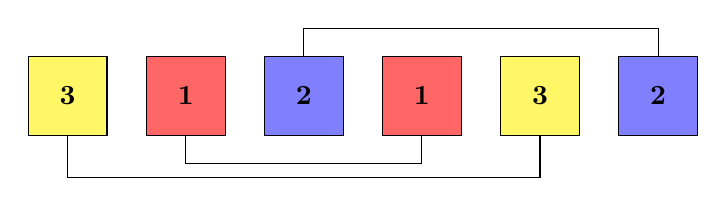
\begin{tikzpicture}
\node (rect) at (0,0) [fill=yellow!60,draw,minimum width=1cm,minimum height=1cm] (p3_1) {\textbf{3}};
\node (rect) at (1.5,0) [fill=red!60,draw,minimum width=1cm,minimum height=1cm] (p1_1) {\textbf{1}};
\node (rect) at (3,0) [fill=blue!50,draw,minimum width=1cm,minimum height=1cm] (p2_1) {\textbf{2}};
\node (rect) at (4.5,0) [fill=red!60,draw,minimum width=1cm,minimum height=1cm] (p1_2) {\textbf{1}};
\node (rect) at (6,0) [fill=yellow!60,draw,minimum width=1cm,minimum height=1cm] (p3_2) {\textbf{3}};
\node (rect) at (7.5,0) [fill=blue!50,draw,minimum width=1cm,minimum height=1cm] (p2_2) {\textbf{2}};
\draw (p3_1.south) -- ([yshift=-15pt]p3_1.south) -- ([yshift=-15pt]p3_2.south) -- (p3_2.south) ;
\draw (p2_1.north) -- ([yshift=10pt]p2_1.north) -- ([yshift=10pt]p2_2.north) -- (p2_2.north) ;
\draw (p1_1.south) -- ([yshift=-10pt]p1_1.south) -- ([yshift=-10pt]p1_2.south) -- (p1_2.south) ;
\end{tikzpicture}  
\end{center}
\caption{L(2,3) arrangement} \label{fig:lang}  
\end{figure}
  
This problem has been generalized to any number $n$ of colors and any number $s$ of blocks having the same color. 
$L(s,n)$ consists in searching for the number of solutions to the Langford problem, up to a symmetry. % ... excepted symmetric ones. 
In November 1967, Martin Gardner presented $L(2,4)$ (two cubes and four colors) as being part of a collection of small mathematical games and he stated that $L(2,n)$ has solutions for all $n$ such that:
\begin{equation}
\text{ solutions for: }
\begin{cases}
n= 4k \\ 
n = 4k-1
\end{cases}
 k \in \mathbb{N}^+
\end{equation}
The central resolution method consists in placing the pairs of cubes, one after the other, on the free places and backtracking if no place is available (see figure~\ref{backtrack} for detailed algorithm).

\begin{table}[t!]
\centering
\[
\begin{tabular}{c r r r}
  \hline
  Instance & Solutions & Method & Computation time\\
  \hline
  \hline
  L(2,3) & 1 &  Miller algorithm & - \\
  L(2,4) & 1 & & - \\ 
  ... & ... & & ...  \\
  L(2,16) & 326,721,800 & & 120 hours  \\
  %\cline{1-3}
  L(2,19) & 256,814,891,280 & & 2.5 years (1999) DEC Alpha \\
  \hline
  \hline
  L(2,20) & 2,636,337,861,200 & Godfrey algorithm & 1 week \\
  %\cline{1-3}
  L(2,23) & 3,799,455,942,515,488 & &  4 days with CONFIIT \\
  %\cline{1-3}
  L(2,24) & 46,845,158,056,515,936 & & 3 months with CONFIIT \\
  L(2,27) & 111,683,611,098,764,903,232 & & 2 days on ROMEO \\
  L(2,28) & 1,607,383,260,609,382,393,152 & & 23 days on ROMEO \\
  \hline
\end{tabular}
\]
\caption{Solutions and time for Langford problem using different methods}
\label{tab:result_base}
\end{table}

The Langford problem has been approached in different ways: discrete mathematics results, specific algorithms, specific encoding, constraint satisfaction problem (CSP), inclusion-exclusion~\ldots~\cite{Mil00,apes-26,Smi00,larsen2009counting}.
In 2004, the last solved instance, $L(2,24)$, was computed by our team \cite{CReSTIC-711} using a specific algorithm. 
Table \ref{tab:result_base} presents the latest results and number of solutions. 
$L(2,27)$ and $L(2,28)$ have just been computed but no details were given. 

The most efficient known algorithms are: the Miller backtrack method, the Godfrey algebraic method and the Larsen inclusion-exclusion method.
The Miller one is based on backtracking and can be modeled as a CSP; it allowed us to move the limit of explicits solutions building up to $L(2,21)$ but combinatorial explosion did not allow us to go further. 
Then, we use the Godfrey method to achieve $L(2,24)$ more quickly and then recompute $L(2,27)$ and $L(2,28)$, presently known as the last instances.
The Larsen method is based on inclusion-exclusion \cite{larsen2009counting}; although this method is effective, practically the Godfrey one is better. 
The latest known work on the Langford Problem is a GPU implementation proposed in \cite{ASS_LGF} in 2015. Unfortunately this study does not provide any performance considerations but just gives the number of solution of $L(2,27)$ and $L(2,28)$.

\section{Miller algorithm}

In this part we present our multi-GPU cluster implementation of the Miller's algorithm. 
This algorithm is very irregular and the repartition have to be done at runtime on our accelerators. 

First, we introduce the backtrack method. 
Then we present our implementation in order to fit the GPUs architecture. 
The last section presents our results. 

\subsection{CSP}

Combinatorial problems are NP-complete \cite{GJ79} and can be described as SATISFIABILITY problems (SAT) using a polynomial transformation. 
They can be transformed into CSP formalism.
A Constraint Satisfaction Problem (CSP), first introduced by Montanari \cite{Mon74}, is defined as a triple $<X,D,C>$ where:
\begin{equation}
\begin{cases}
X=\{X_1,...,X_n\}\text{: a finite set of variables} \\ 
D=\{D_1,...,D_n\}\text{: their finite domains of values}\\
C=\{C_1,...,C_p\}\text{: a finite set of constraints}
\end{cases}
\end{equation}

The goal in this formalism is to assign values in $D$ to $n$-uple $X$ respecting all the $C$ $p$-uple constraints.
This approach is a large field of research. \cite{arbelaez2014gpu} developed \textit{local search} and compares GPU to CPU. 
This first work brings to light that GPU is a real contributor to the global computation speed. \cite{campeotto2014exploring} proposes a solver using \textit{propagator} on a GPU architecture to solve CSP problems. 
\cite{jenkins2011lessons} cares about GPU weak points, loading bandwidth and global memory latency.

%\subsection{CSP parallel resolution}
%\label{sec:CSP_resolution}

Considering a basic approach, combinatorial problems formed into CSP can be represented as a tree search. Each level corresponds to a given variable, with values in its domain. Leaves of the tree correspond to a complete assignment (all variables are set). If it meets all the constraints this assignment is called an acceptor state. Depending on the constraints set, the satisfiability evaluation can be made either on complete or partial assignment.
%
%There are many ways to browse the tree and find the solutions: \emph{backtracking}, \emph{forward-checking}, \emph{backjumping}, etc. 
%We limit our method to the naive \emph{backtrack} resolution. We chose to evaluate the variables and their values in a static order; in a depth-first manner, the solution is built incrementally and if a partial assignment can be aborted, the branch is cut. A solution is found each time a leaf is reached.
%% presents a backtrack search with the previous CSP representation.
%
%The recommendation for performance on GPU accelerator is to use non test-based programs.
%Due to its irregularity, the basic \emph{backtracking} algorithm is suppose not to suit the GPU architecture.
%Thus a vectorized version is given when evaluating the assignments at the leaves' level, with one of the two following ways: assignments can be prepared on each tree node or totally set on final leaves before testing the satisfiability of the built solution, Fig.\ref{fig:algos}.
%
%\begin{figure}[htbf]
%\begin{minipage}[b]{0.45\linewidth}
%\begin{verbatim}
%for variable_1 
%   assignment
%   for variable_2
%      assignment
%      ...
%         for variable_n
%            assignment
%            test
%\end{verbatim}
%\end{minipage}
%\begin{minipage}[b]{0.45\linewidth}
%\begin{verbatim}
%for variable_1 
%   for variable_2
%   ...
%      for variable_n
%         assignments
%         test
%         
%         
%\end{verbatim}
%\end{minipage} 
%\caption{CSP regularized algorithms}
%\label{fig:algos}
%\end{figure} 
%
%With this method it is necessary to browse the entire tree but this requires using all the search space and it is too time-consuming.
%
%In order to overcome this we divide the work between CPU and GPU. The CPU generates some levels of the tree and creates tasks. Then GPU and CPU cores divide up the workload in order to achieve the generation on the latest levels of the tree. With this method, inconsistent branches can be cut on highest level and GPU/CPU cores only compute possibly consistent tasks.
%
%This representation enables a server-client model to distribute the tasks: the server generates independent sub-problems at a chosen depth in the tree, treated by clients. 
%Each client decomposes the sub-problem into tasks, distributed over the GPU/CPU cores, Fig.\ref{fig:parallel}.
%
%\begin{figure}[htbf]
%\centering 
%\includegraphics[scale=0.9]{figures/graphe_repartition}   
%\caption{Server client distribution} \label{fig:parallel}    
%\end{figure} 
%
%With this method numerous branches have been cut from the main tree during generation stage and GPU/CPU tasks are faster due to their lower depth. Despite the combinatorial explosion of this kind of problem, we can consider solving CSP in a massively parallel manner on multiGPU clusters.

\subsection{Backtrack resolution}

As presented above the Langford problem is known to be a highly irregular combinatorial problem. 
We first present here the general tree representation and the ways we regularize the computation for GPUs.
Then we show how to parallelize the resolution over a multi-GPU cluster.

\subsubsection{Langford's problem tree representation}
\label{sec:LGF_resolution}
%In~\cite{HKS02}, we propose to formalize the Langford problem as a CSP  ({\it Constraint Satisfaction Problem}), first introduced by Montanari in \cite{Mon74}, and show that an efficient parallel resolution is possible. 
As explained, CSP formalized problems can be transformed into tree evaluations. %represented as trees. 
%The tree Here we intend to develop a specific algorithm taking into account the conclusion of our previous studies (memory management of memory and load balance) and transfer the tasks resolution into GPUs.\\
%\begin{figure}[htb]
%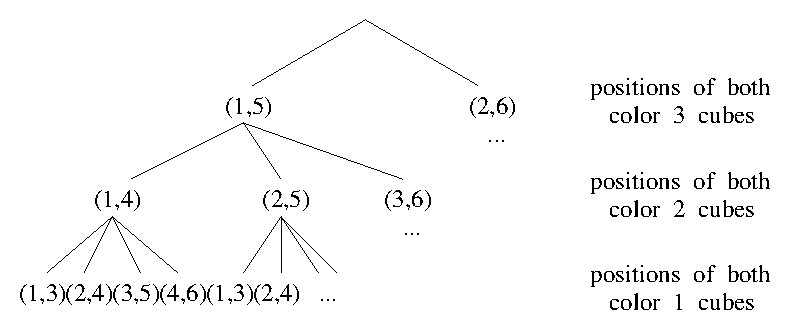
\includegraphics[scale=.65]{\locpath/figures/langford/arbre_en}
%\end{figure}
\begin{figure}[t!]
\centering
\resizebox {\columnwidth} {!} {
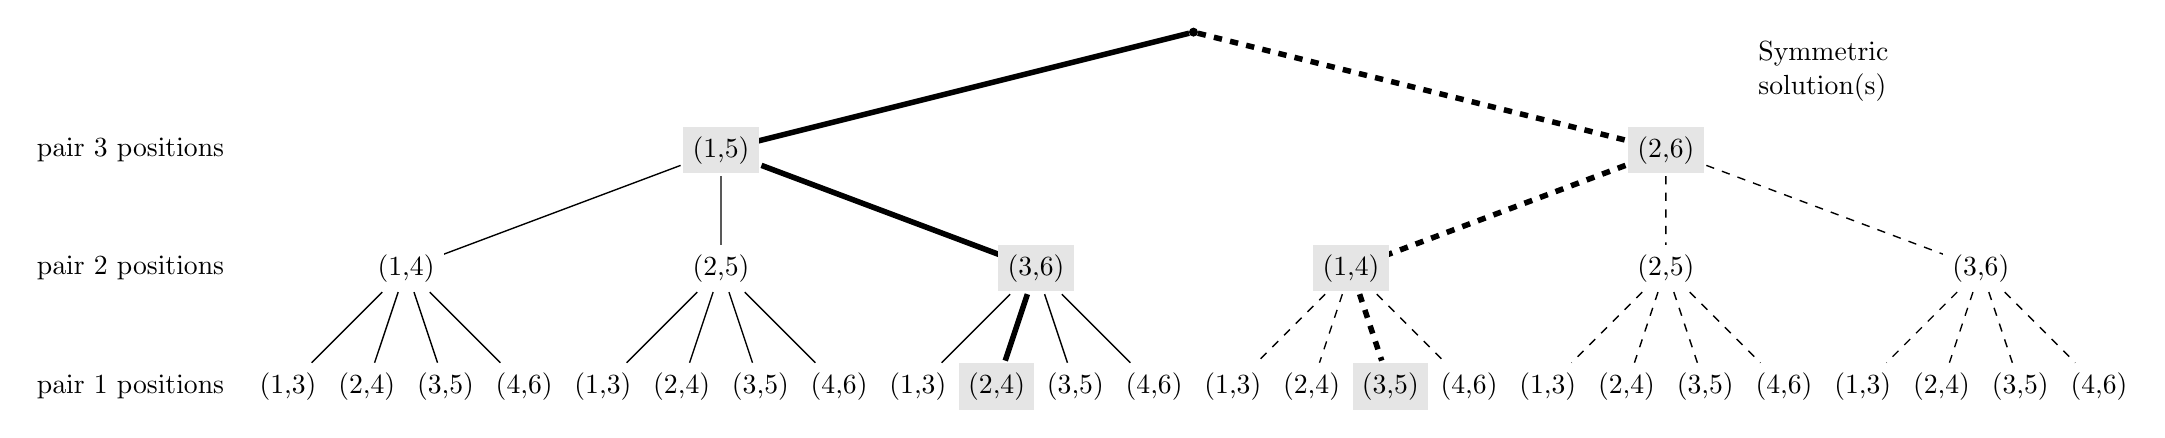
\begin{tikzpicture}[sibling distance=12cm]
\node at (-13.5,-1.5) {pair 3 positions};
\node at (-13.5,-3) {pair 2 positions};
\node at (-13.5,-4.5) {pair 1 positions};
\node [align=left] at (8,-.5) {Symmetric\\solution(s)};
\node  [circle,draw,fill,inner sep=1] {}
  child [line width=2pt] { [sibling distance=4cm] node [fill=black!10] {(1,5)}
    child [line width=.5pt] { [sibling distance=10mm] node [fill=white] {(1,4)}
      child {node {(1,3)}}
      child {node {(2,4)}}
      child {node {(3,5)}}
      child {node {(4,6)}}
    }
    child [line width=.5pt] { [sibling distance=10mm] node [fill=white] {(2,5)}
      child {node {(1,3)}}
      child {node {(2,4)}}
      child {node {(3,5)}}
      child {node {(4,6)}}
    }
    child { [sibling distance=10mm] node [fill=black!10] {(3,6)}
      child [line width=.5pt] {node {(1,3)}}
      child {node [fill=black!10] {(2,4)}}
      child [line width=.5pt] {node {(3,5)}}
      child [line width=.5pt] {node {(4,6)}}
    }
  }
  child [dashed,line width=2pt] { [sibling distance=4cm] node [fill=black!10] {(2,6)}
    child { [sibling distance=10mm] node [fill=black!10] {(1,4)}
      child [line width=.5pt] {node {(1,3)}}
      child [line width=.5pt] {node {(2,4)}}
      child {node [fill=black!10] {(3,5)}}
      child [line width=.5pt] {node {(4,6)}}
    }
    child [line width=.5pt] { [sibling distance=10mm] node [fill=white] {(2,5)}
      child {node {(1,3)}}
      child {node {(2,4)}}
      child {node {(3,5)}}
      child {node {(4,6)}}
    }
    child [line width=.5pt] { [sibling distance=10mm] node [fill=white] {(3,6)}
      child {node {(1,3)}}
      child {node {(2,4)}}
      child {node {(3,5)}}
      child {node {(4,6)}}
    }
  }
;
\end{tikzpicture}
}
\caption{Search tree for $L(2,3)$}
\label{fig:arbre}
\end{figure}
In order to solve $L(2,n)$, we consider a tree of height $n$: see example of $L(2,3)$ in figure~\ref{fig:arbre}.

\begin{itemize}   
\item[-] Every level of the tree corresponds to a color.
\item[-] Each node of the tree corresponds to the placement of a pair of cubes without worrying about the other colors. Color $p$ is represented at depth $n-p+1$, where the first node corresponds to the first possible placement (positions 1 and $p+2$) and $i^{th}$ node corresponds to the placement of the first cube of color $p$ in position $i, \ i \in [1, \ 2n-1-p]$.
\item[-] Solutions are leaves generated without any placement conflict.
\item[-] As we consider the solution up to a symmetry, the left part is represented dashed and is in fact not traversed.
\end{itemize}

There are many ways to browse the tree and find the solutions: \emph{backtracking}, \emph{forward-checking}, \emph{backjumping}, etc \cite{prosser93hybrid}. 
We limit our study to the naive \emph{backtrack} resolution and choose to evaluate the variables and their values in a static order; in a depth-first manner, the solutions are built incrementally and if a partial assignment can be aborted, the branch is cut. A solution is found each time a leaf is reached.
% presents a backtrack search with the previous CSP representation.

The recommendation for performance on GPU accelerators is to use non test-based programs.
Due to its irregularity, the basic \emph{backtracking} algorithm, presented on figure~\ref{backtrack}, is not supposed to suit the GPU architecture.
Thus a vectorized version is given when evaluating the assignments at the leaves' level, with one of the two following ways: assignments can be prepared on each tree node or totally set on final leaves before testing the satisfiability of the built solution (figure~\ref{regularized}).

\begin{figure}[t!]
\begin{minipage}[b]{0.45\linewidth}
\footnotesize
\begin{verbatim}
while not done do
 test pair            <- test
 if successful then 
   if max depth then
     count solution
     higher pair	                  
   else
     lower pair       <- remove
 else
   higher pair        <- add
\end{verbatim}
\caption{Backtrack algorithm}\label{backtrack}
\end{minipage}
\begin{minipage}[b]{0.45\linewidth}
\footnotesize
\begin{verbatim}
for pair 1 positions
  assignment                   <- add
  for pair 2 positions
    assignment                 <- add
    for ...
      for pair n positions
        assignment             <- add
        if final test ok then  
          count solution
\end{verbatim}
\caption{Regularized algorithm}\label{regularized}
\end{minipage}
\end{figure}

\subsubsection{Data representation}

\begin{figure}[t!]
\begin{minipage}[b]{0.40\linewidth}
\centering
\includegraphics[width=\columnwidth]{\locpath/figures/langford/positions_lgf}
\caption{ Bitwise representation of pairs positions in $L(2,3)$} \label{fig:comb1}
\end{minipage}
\hfill
\begin{minipage}[b]{0.55\linewidth}
\centering
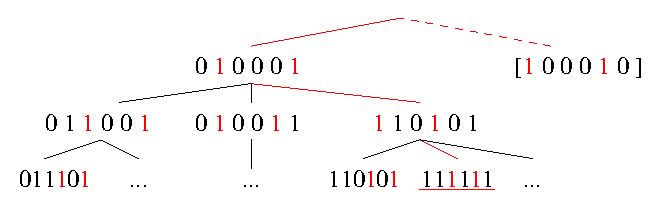
\includegraphics[width=\columnwidth]{\locpath/figures/langford/pos_lgf_v2}
\caption{Bitwise representation of the Langford $L(2,3)$ placement tree}\label{fig:pos_lgf}
\end{minipage}
\end{figure}

In order to count every Langford problem solution, we first identify all possible combinations for one color without worrying about the other ones. 
Each possible combination is coded within an integer, one bit to 1 corresponding to a cube presence, a 0 to its absence. This is what we called a \emph{mask}.
This way figure~\ref{fig:comb1} presents the possible combinations to place the one, two and three weight cubes for the $L(2,3)$ Langford instance.

Furthermore the masks can be used to evaluate the partial placements of a chosen set of colors: all the 1 correspond to occupied positions; the assignment is consistent \emph{iff} there are as many 1 as the number of cubes set for the assignment. 

With the aim to find solutions, we just have to go all over the tree and \emph{sum} one combination of each of the colors: a solution is found \emph{iff} all the bits of the sum are set to 1. 

Each route on the tree can be evaluated individually and independently; then it can be evaluated as a thread on the GPU.
This way the problem is massively parallel and can be, indeed, computed on GPU. figure~\ref{fig:pos_lgf} represents the tree masks' representation.

\subsubsection{Specific operations and algorithms}

Three main operations are required in order to perform the tree search. 
%The first one, allowing to check if a pair can be added to a given partial assignment, is only necessary for the original backtrack scheme.
%The second one, used for both backtrack and regularized methods, aims to add a pair to a given assignment. 
The first one, used for both backtrack and regularized methods, aims to add a pair to a given assignment. 
The second one, allowing to check if a pair can be added to a given partial assignment, is only necessary for the original backtrack scheme.
The last one is used for testing if a global assignment is an available solution: it is involved in the regularized version of the Miller algorithm.

\begin{figure}[t!]
\begin{minipage}[b]{0.5\linewidth}
\centering
\includegraphics[scale=.5]{\locpath/figures/langford/test_gen}
\caption{Testing and adding position} \label{fig:test_et}
\end{minipage}
\begin{minipage}[b]{0.5\linewidth}
\centering 
\includegraphics[scale=.75]{\locpath/figures/langford/graphe_repartition}   
\caption{Server client distribution} \label{fig:parallel} 
\end{minipage}
\end{figure}

\paragraph{Add a pair: }
Top of figure~\ref{fig:test_et} presents the way to add a pair to a given assignment.
With a \emph{binary OR}, the new mask contains the combination of the original mask and of the added pair.
This operation can be performed even if the position is not available for the pair (however the resulting mask is inconsistent). 

\paragraph{Test a pair position: }
On the bottom part of the same figure, we test the positioning of a pair on a given mask. 
For this, it is necessary to perform a \emph{binary AND} between the mask and the pair.
\begin{itemize}
	\item[] $=0$: \emph{success}, the pair can be placed here
	\item[] $\neq0$: \emph{error}, try another position
\end{itemize}

\paragraph{Final validity test: }
The last operation is for \emph{a posteriori} checking. For example the mask $101111$, corresponding to a leaf of the tree, is inconsistent and should not be counted among the solutions.
The final placement mask corresponds to a solution \emph{iff} all the places are occupied, which can be tested as $\neg mask = 0$. % \rightarrow solution$ else $inconsistent$.
%We performed a \emph{binary not} on the mask. If there is a zero, so the mask is inconsistent, result will be different of zero. If the mask is full of $1$, result is zero, so we can add one to the number of solutions.
\\

Using this data representation, 
we implemented both \emph{backtrack} and \emph{regularized} versions of the Miller algorithm, as presented in figure~\ref{backtrack} and \ref{regularized}.
% C'est là que je veux changer la structure ....
%: the original backtrack for CPU computation and the regularized one for GPUs.
%As we have seen above, the regularized algorithm is unsuitable due to combinatorial explosion, that is why we use the hybrid method on a distributed architecture.
\\
The next section presents the way we hybridize these two schemes in order to get an efficient parallel implementation of the Miller algorithm.

%%%%%%%%%%%%%%%%%%%%%%%%%%%%%%%%%%%%%%%%
\subsection{Hybrid parallel implementation}
\label{section:parallel_backtrack}
This part presents our methodology to implement Miller's method on a multiGPU cluster.

\paragraph{Tasks generation: }
In order to parallelize the resolution we have to generate tasks. 
Considering the tree representation, we construct tasks by fixing the different values of a first set of variables [pairs] up to a given level. Choosing the development level allows to generate as many tasks as necessary. This leads to a \textit{Finite number of Irregular and Independent Tasks} (\emph{FIIT} applications \cite{krajecki1999object}). 

\paragraph{Cluster parallelization: } 
The generated tasks are independent and we spread them in a client-server manner: a server generates them and makes them available for clients. As we consider the cluster as a set of CPU-GPU(s) machines, the clients are these machines. 
At the machines level, the role of the CPU is, first, to generate work for the GPU(s): it has to generate sub-tasks, by continuing the tree development as if it were a second-level server, and the GPU(s) can be considered as second-level client(s). \\
The sub-tasks generation, at the CPU level, can be made in parallel by the CPU cores. Depending on the GPUs number and their computation power the sub-tasks generation rhythm may be adapted, to maintain a regular workload both for the CPU cores and GPU threads: some CPU cores, not involved in the sub-tasks generation, could be made available for sub-tasks computing.\\
This leads to the 3-level parallelism scheme presented in figure~\ref{fig:parallel}, where $p$, $q$ and $r$ respectively correspond to: ($p$) the server-level tasks generation depth, ($q$) the client-level sub-tasks generation one, ($r$) the remaining depth in the tree evaluation, \textit{i.e.} the number of remaining variables to be set before reaching the leaves.  

\paragraph{\emph{Backtrack} and \emph{regularized} methods hybridization: } 
The Backtrack version of the Miller algorithm suits CPU execution and allows to cut branches during the tree evaluation, reducing the search space and limiting the combinatorial explosion effects. A regularized version had to be developed, since GPUs execution requires synchronous execution of the threads, with as few branching divergence as possible; however this method imposes to browse the entire search space and is too time-consuming. \\
We propose to hybridize the two methods in order to take advantage of both of them for the multiGPU parallel execution: 
for tasks and sub-tasks generated at sever and client levels, the tree development by the CPU cores is made using the backtrack method, cutting branches as soon as possible [and generating only possible tasks]; when computing the sub-tasks generated at client-level, the CPU cores involved in the sub-tasks resolution use the backtrack method and the GPU threads the regularized one. 

%With this method it is necessary to browse the entire tree but this requires using all the search space and it is too time-consuming.

%In order to overcome this we divide the work between CPU and GPU. The CPU generates some levels of the tree and creates tasks. Then GPU and CPU cores divide up the workload in order to achieve the generation on the latest levels of the tree. 
%With this method, inconsistent branches can be cut on highest level and GPU/CPU cores only compute possibly consistent tasks.

%This representation enables a server-client model to distribute the tasks: the server generates independent sub-problems at a chosen depth in the tree, treated by clients. 
%Each client decomposes the sub-problem into tasks, distributed over the GPU/CPU cores, Fig.~\ref{fig:parallel}.

%By doing so numerous branches have been cut from the main tree during generation stage and GPU/CPU tasks are faster due to their lower depth. Despite the combinatorial explosion of this kind of problem, we can consider solve it in a massively parallel manner on multiGPU clusters.
 
%The tree representation allows to generate tasks at a chosen level, which leads to a \textit{Finite number of Irregular and Independent Tasks} (\emph{FIIT} applications \cite{krajecki1999object}).
%We set up a server-client distribution. The server, client and GPU parts have their own development depth, respectively $p$, $q$ and $r$, $p+q+r=n$, Fig.~\ref{fig:parallel}.
%\begin{itemize}
%\item \texttt{Server} generates sub-problems by placing $p$ pairs on masks with the $backtrack$ algorithm.
%\item \texttt{Client} starts with a mask generated by the server and produces tasks by adding $q$ pairs in the initial mask, with the $backtrack$ algorithm. Then the client creates specific tasks by pre-computing the available positions for placing pairs. For example with the $10100110$ mask the second pair can be placed on only two positions, $01001000$ and $00001001$, that match positions 2-5 and 5-8. Instead of browsing all the 5 positions and test, the GPU just has to try 2 positions for this pair. Thus we greatly reduce the GPU load computation.
%\item \texttt{CPUs and GPUs} can compute in competition. Whereas CPUs use standard backtrack, GPUs generate leaves using the regularized method and adding successive pairs on their masks without any test.  
%\end{itemize}

\subsection{Experiments tuning}

In order to take advantage of all the computing power of the GPU we have to refine the way we use them: this section presents the experimental study required to choose optimal settings. This tuning allowed us to prove our proposal on significant instances of the Langford problem.

\paragraph{Registers, blocks and grid: }

In order to use all GPUs capabilities, the first way was to fill the blocks and grid. To maximize occupancy (ratio between active warps and the total number of warps) NVIDIA suggests to use 1024 threads per block to improve GPU performances and proposes a CUDA occupancy calculator\footnote{\url{http://developer.download.nvidia.com/compute/cuda/CUDA_Occupancy_calculator.xls}}. But, confirmed by the Volkov's results\cite{Volkov}, we experimented that better performances may be obtained using lower occupancy. Indeed, another critical criterion is the inner GPU registers occupation. 
The optimal number of registers ($57$ registers) is obtained by setting 9 pairs placed on the client for $L(2,15)$, thus 6 pairs are remaining for GPU computation.

\begin{figure}[t!]
\centering
\includegraphics[scale=.4]{\locpath/figures/langford/graphe_15_9}
\caption{Time depending on grid and block size on $n=15$}
\label{f7}
\end{figure}

In order to tune the blocks and grid sizes, we performed tests on the ROMEO architecture. 
%0 With this value we obtained an optimized number of registers by thread . 
Figure~\ref{f7} represents the time in relation with the number of blocks per grid and the number of threads per block. 
The most relevant result, observed as a local minimum on the 3D surface, is obtained near 64 or 96 threads per block; for the grid size, the limitation is relative to the GPU global memory size.
It can be noted that we do not need shared memory because their are no data exchanges between threads. 
This allows us to use the total available memory for the L1 cache for each thread.

\paragraph{Streams:}
A client has to prepare work for GPU. There are four main steps: generate the tasks, load them into the device memory, process the task on the GPU and then get the results.

\begin{figure}[t!]
\begin{minipage}[b]{0.48\linewidth}
\centering
\includegraphics[width=\columnwidth]{\locpath/figures/langford/streams.jpeg}
\caption{Computing time depending on streams number}
\label{fig:streams}
\end{minipage}
\hfill
\begin{minipage}[b]{0.48\linewidth}
\centering
\includegraphics[width=\columnwidth]{\locpath/figures/langford/graphe_cores.pdf}
\caption{CPU cores optimal distribution for GPU feeding}\label{cores_rep}
\end{minipage}
\end{figure}

CPU-GPU memory transfers cause huge time penalties (about 400 cycles latency for transfers between CPU memory and GPU \emph{device memory}). 
At first, we had no overlapping between memory transfer and kernel computation because the tasks generation on CPU was too long compared to the kernel computation.
To reduce the tasks generation time we used OpenMP in order to use the eight available CPU cores.
Thus CPU computation was totally hidden by memory transfers and GPU kernel computation. We tried using up to 7 streams; as shown by figure~\ref{fig:streams}, using only two simultaneous streams did not improve efficiency because the four steps did not overlap completely; the best performances were obtained with three streams; the slow increase in the next values is caused by synchronization overhead and CUDA streams management.

\paragraph{Setting up the server, client and GPU depths: }
We now have to set the depths of each actor, server $(p)$, client $(q)$ and GPU $(r)$ (see figure~\ref{fig:parallel}).

First we set the $r = 5$ for large instances because of the GPU limitation in terms of registers by threads, exacerbated by the use of numerous $64bits$ integers. For $r \geq 6$, we get too many registers (64) and for $r \leq 4$ the GPU computation is too fast compared to the memory load overhead.

Clients are the buffers between the server and the GPUs: 
$q = n - p- r$.
So we have conducted tests by varying the server depth, $p$. The best result is obtained for $p=3$ and performance decreases quickly for higher values. This can be explained since more levels on the server generates smaller tasks; thus GPU use is not long enough to overlap memory exchanges.
% because with more levels on the server, tasks are smaller and then the GPU work is not long enough in view of memory exchanges.

\paragraph{CPU: Feed the GPUs and compute}
The first work of CPU cores is to prepare tasks for GPU so that we can generate overlapping between memory load and kernel computation. 
In this configuration using eight cores to generate GPU tasks under-uses CPU computation power. 
It is the reason why we propose to use some of the CPU cores to take part of the sub-problems treatment. 
Figure~\ref{cores_rep} represents computation time in relation with different task distributions between CPU and GPU.
We experimentally demonstrated that only 4 or 5 CPU cores are enough to feed GPU, the other ones can be used to perform backtrack resolution in competition with GPUs.

\subsection{Results}

\paragraph{Regularized method results}
We now show the results obtained for our massively parallel scheme using the previous optimizations, comparing the computation times of successive instances of the Langford problem. 
These tests were performed on 20 nodes of the ROMEO supercomputer, hence 40 CPU/GPU machines.

The previous limit with Miller's algorithm was $L(2,19)$, obtained in 1999 after 2.5 years of sequential effort and at the same time after 2 months with a distributed approach\cite{Mil00}. 
Our computation scheme allowed us to obtain it in less than 4 hours (Table \ref{tab:result_base_regu}), this being not only due to Moore law progress.\\
Note that the computation is 1.6 faster with CPU+GPU together than using 8 CPU cores. 
In addition, the GPUs compute $200000\times$ more nodes of the search tree than the CPUs, with a faster time.

\begin{table}[t!]
\begin{subfigure}[b]{0.5\linewidth}
\centering
\begin{tabular}{l r r r}
					\hline
					$n$ & CPU (8c) &  GPU (4c) +  &  \hspace*{-.8em}CPU (4c) \\
					\hline
					\hline
					15	& 2.5 & 1.5 & \\
					16  & 21.2 &14.3 & \\
					17  & 200.3 &120.5 &\\
					18  & 1971.0 &1178.2 &\\
					19  & 22594.2 & 13960.8 & \\ 
					\hline
\end{tabular}
\caption{Regularized method (seconds)}
\label{tab:result_base_regu}
\end{subfigure}
\begin{subfigure}[b]{0.5\linewidth}
\centering
\begin{tabular}{ l r r r }
					\hline
					$n$ & CPU (8c) &  GPU (4c) +  &  \hspace*{-.8em}CPU (4c) \\
					\hline
					\hline
					17  & 29.8 & 7.3&\\
					18  & 290.0 & 73.6&\\
					19  & 3197.5 & 803.5& \\
					20  & -- & 9436.9 &\\
					21  & -- & 118512.4& \\ 
					\hline
\end{tabular}	
\caption{Backtrack  (seconds)}
\label{tab:result_backtrack}
\end{subfigure}
\caption{Comparison between multi-core processors and GPUs for regularized and backtrack method}
\end{table}

The computation time between two different consecutive instances being multiplied by $10$ approximately, this could allow us to obtain $L(2,20)$ in a reasonable time.


\paragraph{Backtracking on GPUs}

It appears at first sight that using backtracking on GPUs without any regularization is a bad idea due to threads synchronization issues.
But in order to compare CPU and GPU computation power in the same conditions we decide to implement the original backtrack method on GPU (see figure~\ref{backtrack}) with only minor modifications.
In these conditions we observe very efficient work of the NVIDIA scheduler, which perfectly handles threads de-synchronization.
Thus we use the same server-client distribution as in \ref{section:parallel_backtrack}, each client generates masks for both CPU and GPU cores. 
The workload is then statically distributed on GPU and CPU cores.
Executing the backtrack algorithm on a randomly chosen set of sub-problems allowed us to set the GPU/CPU distribution ratio experimentally to 80/20\%.

The experiments were performed on 129 nodes of the ROMEO supercomputer, hence 258 CPU/GPU machines and one node for the server. 
Table \ref{tab:result_backtrack} shows the results with this configuration. 
This method first allowed us to perform the computation of $L(2,19)$ in less than 15 minutes, $15\times$ faster than with the regularized method; then, we pushed the limitations of the Miller algorithm up to $L(2,20)$ in less than 3 hours and even $L(2,21)$ in about $33$ hours\footnote{Even if this instance has no interest since it is known to have no solution}.

This exhibits the ability of the GPU scheduler to manage highly irregular tasks. 
It proves that GPUs are adapted even to solve combinatorial problems, which they were not supposed to be.

\section{Godfrey's algebraic method}
The previous part presents the Miller algorithm for the Langford problem, this method cannot achieve bigger instances than the $L(2,21)$.\\
An algebraic representation of the Langford problem has been proposed by M. Godfrey in 2002.
In order to break the limitation of $L(2,24)$ we already used this very efficient problem specific method.
In this part we describe this algorithm and optimizations, and then our implementation on multiGPU clusters.
\subsection{Method description}
Consider $L(2,3)$ and $X=(X_1,X_2,X_3,X_4,X_5,X_6)$. 
It proposes to modelize $L(2,3)$ by: 
\begin{equation}
\begin{aligned}
F(X,3) = & (X_1X_3+X_2X_4+X_3X_5+X_4X_6)\times \\
& (X_1X_4+X_2X_5+X_3X_6)\times\\
& (X_1X_5+X_2X_6)
\end{aligned}
\end{equation}
In this approach each term represents a position of both cubes of a given color and a solution to the problem corresponds to a term developed as $(X_1X_2X_3X_4X_5X_6)$; thus the number of solutions is equal to the coefficient of this monomial in the development. 
More generally, the solutions to $L(2,n)$ can be deduced from $(X_1X_2X_3X_4X_5...X_{2n})$ terms in the development of $F(X,n)$.

If \ \ $G(X,n) = X_1 ... X_{2n} F(X,n)$ then it has been shown that: 

\begin{equation}
\sum\limits_{(x_1,...,x_{2n}) \in \{-1,1\}^{2n}} G(X,n)_{(x_1,...,x_{2n})} =  2^{2n+1}L(2,n)
\end{equation}

So \hspace*{2cm}
\begin{equation}
\sum\limits_{(x_1,...,x_{2n}) \in \{-1,1\}^{2n}} \big( \prod\limits_{i=1}^{2n} x_i \big) \prod\limits_{i=1}^{n} \sum\limits_{k=1}^{2n-i-1} x_kx_{k+i+1} = 2^{2n+1} L(2,n)
\end{equation}

\noindent That allows to get $L(2,n)$ from polynomial evaluations.
The computational complexity of $L(2,n)$ is of $O(4^n\times n^2)$ and an efficient big integer arithmetic is necessary. 
This principle can be optimized by taking into account the symmetries of the problem and using the Gray code: these optimizations are described below.

\subsection{Optimizations}
Some works focused on finding optimizations for this arithmetic method\cite{CReSTIC-1154}. 
Here we explain the symmetric and computation optimizations used in our algorithm.

\subsubsection{Evaluation parity: }
As $[F(-X,n) = F(X,n)]$, $G$ is not affected by a global sign change. 
In the same way the global sign does not change if we change the sign of each pair or impair variable.

Using these optimizations we can set the value of two variables and accordingly divide the computation time and result size by four.

\subsubsection{Symmetry summing: }
In this problem we have to count each solution up to a symmetry; thus for the first pair of cubes we can stop the computation at half of the available positions considering 

\noindent $S'_1(x) = \sum_{k=1}^{n-1}x_kx_{k+2}$ instead of $S_1(x) = \sum_{k=1}^{2n-2} x_kx_{k+2}$.
The result is divided by 2. 

\subsubsection{Sums order: }
Each evaluation of $ S_i(x) = \sum_{k=1}^{2n-i-1} x_kx_{k+i+1} $, before multiplying might be very important regarding to the computation time for this sum. 
Changing only one value of $ x_i $ at a time, we can recompute the sum using the previous one without global re-computation. 
Indeed, we order the evaluations of the outer sum using Gray code sequence. 
Then the computation time is considerably reduced.  

Based on all these improvements and optimizations we can use the Godfrey method in order to solve huge instances of the Langford problem. 
The next section develops the main issues of our multiGPU architecture implementation. 

\subsection{Implementation details}
In this part we present the specific adaptations required to implement the Godfrey method on a multiGPU architecture.

\subsubsection{Optimized big integer arithmetic: }

In each step of computation, the value of each $S_i$ can reach $2n-i-1$ in absolute value, and their product can reach $\frac{(2n-2)!}{(n-2)!}$. 
As we have to sum the $S_i$ product on $2^{2n}$ values, in the worst case we have to store a value up to $2^{2n}\frac{(2n-2)!}{(n-2)!}$, which corresponds to $10^{61}$ for $n=28$, with about 200 bits.

So we need few big integer arithmetic functions. After testing existing libraries like GMP for CPU or CUMP for GPU, we came to the conclusion that they implement a huge number of functionalities and are not really optimized for our specific problem implementation: product of "small" values and sum of "huge" values. 

Finally, we developed a light CPU and GPU library adapted to our needs.
In the sum for example, as maintaining carries has an important time penalty, we have chosen to delay the spread of carries by using buffers: carries are accumulated and spread only when useful (for example when the buffer is full).
Figure~\ref{fig:big-integer} represents this big integer handling.
\begin{figure}[htbp]
\centering
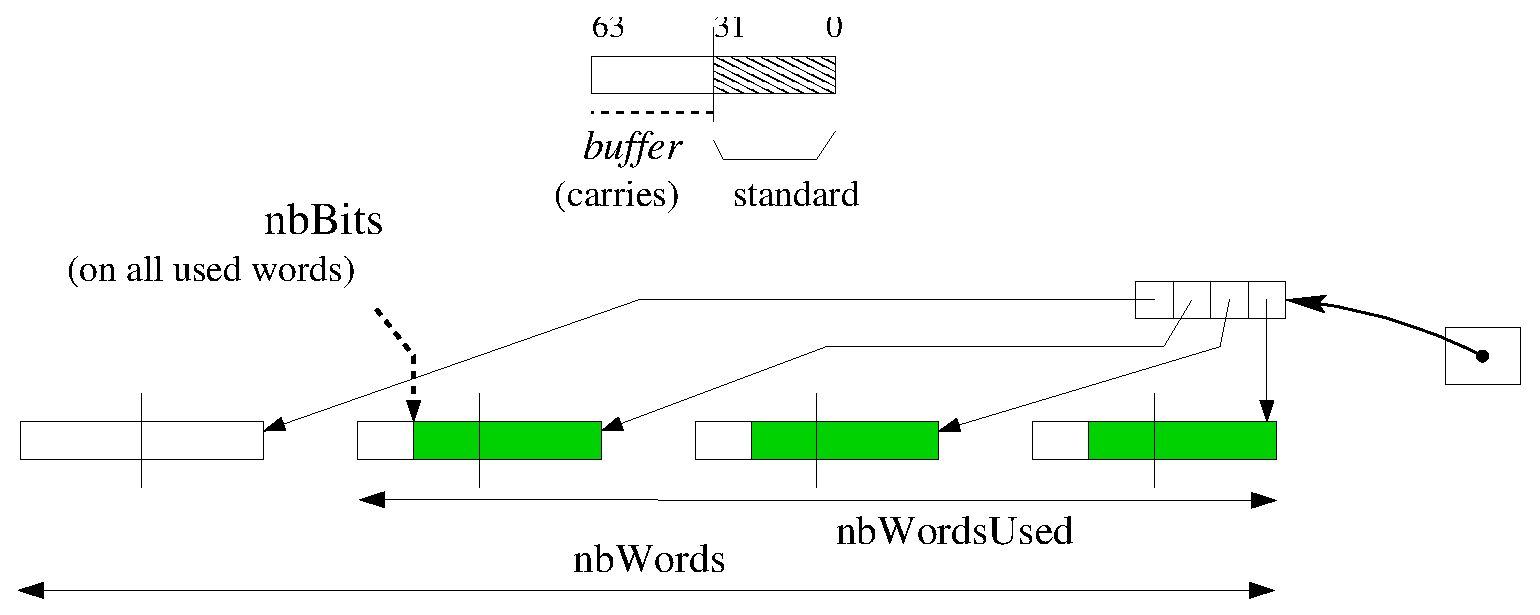
\includegraphics[scale=.5]{\locpath/figures/langford/lgf_grands_entiers}
\caption{Big integer representation, 64 bits words}
\label{fig:big-integer}
\end{figure}


\subsubsection{Gray sequence in memory: }
The Gray sequence cannot be stored in an array because it would be too large (it would contain $2^{2n}$ byte values). This is the reason why only one part of the Gray code sequence is stored in memory and the missing terms are directly computed from the known ones using arithmetic considerations.
The size of the stored part of the Gray code sequence is chosen to be as large as possible to be contained in the processor's cache memory, the L1 cache for the GPUs threads: so the accesses are fastened and the computation of the Gray code is optimized.
For an efficient use of the E5-2650 v2 ROMEO's CPUs, which disposes of 20 MB of level-3 cache, the CPU Gray code sequence is developed recursively up to depth 25. For the K20Xm ROMEO's GPUs, which dispose of 8 KB of constant memory, the sequence is developed up to depth 15. The rest of the memory is used for the computation itself. 
%As the Gray sequence is not entirely stored in memory, 
%As we show, all the gray sequence is not in memory, in order to compute the next value when the array is exceeded a modulus method is used for recompute the next value.

\subsubsection{Tasks generation and computation: }
\label{sec:tasks}

In order to perform the computation of the polynomial, two variables can be set among the $2n$ available. For the tasks generation we choose a number $p$ of variables to generate $2^p$ tasks by developing the evaluation tree to depth $p$.\\
 
 
The tasks are spread over the cluster, either synchronously or asynchronously.

\paragraph{Synchronous computation: }
A first experiment was carried out with an MPI distribution of the tasks of the previous model. 
Each MPI process finds its tasks list based on its process \textit{id}; then converting each task number into binary gives the task's initialization. 
The processes work independently; finally the root process ($id=0$) gathers all the computed numbers of solutions and sums them.

\paragraph{Asynchronous computation: }
\label{section:asynchronous}
In this case the tasks can be computed independently. 
As with the synchronous computation, the tasks' initializations are retrieved from their number. 
Each machine can get a task,  compute it, and then store its result; then when all the tasks have been computed, the partial sums are added together and the total result is provided. 

%In this case if a task is cancel due to machine error or another problem, it can be restart without compromising the end of execution.

%\subsubsection{Efficient computation}
%The computation of any task can be summarized in the four following steps:
%\begin{itemize}
%\item First it is necessary to initialize the task: with depth level $p$, $X_1=X_2=1$ and the next $p$ variables are assigned to $1$ or $-1$ depending on the task's id. The following ones are set to $1$ for example.
%\item Secondly it is necessary to set the value of each $S_i$ with the sum of $X_kX_{k + i + 1}$.
%\item Then CPU and GPU, concurrently working, go through all of the Gray sequence on the remaining $2n-p-2$ variables, by updating the $S_i$ and sum their product at each step.
%\item Finally the CPU cores computed results are summed over a shared variable; the GPU sub-tasks results are copied back and then summed with the global result.
%\end{itemize}

\subsection{Experimental settings}
This part presents the experimental context and methodology, and the way the experiments were carried out.
This study has similar goals as for the Miller's resolution experiments.

\subsubsection{Experimental methodology: }
We present here the way the experimental settings were chosen.
Firstly we define the tasks distribution, secondly we set the number of threads per GPU block; finally, we set the CPU/GPU distribution.

\paragraph{Tasks distribution depth: }
This value being set it is important to get a high number of blocks to maintain sufficient GPU load.
Thus we have to determine the best number of tasks for the distribution. As presented in part \ref{sec:tasks} the number $p$ of bits determines $2^p$ tasks. On the one hand, too many tasks are a limitation for the GPU that cannot store all the tasks in its 6GB memory. On the other hand, not enough tasks means longer tasks and too few blocks to fill the GPU grid. figure~\ref{fig:graphe_prof} shows that for the $L(2,23)$ instance the best task number is with generation depth 28.

\paragraph{Number of threads per block: }
In order to take advantage of the GPU computation power, we have to determine the threads/block distribution. Inspired by our experiments with Miller's algorithm we know that the best value may appear at lower occupancy. We perform tests on a given tasks set varying the threads/block number and grid size associated. 
Figure~\ref{fig:graphe_threads} presents the tests performed on the $n=20$ problem: the best distribution is around $128$ threads per block. 
\begin{figure}[t!]
\centering 
\includegraphics[scale=.55]{\locpath/figures/langford/graphe_threads}
\caption{$L(2,20)$, number of threads per block}
\label{fig:graphe_threads}
\end{figure}

\begin{figure}[t!]
\begin{subfigure}[b]{0.5\linewidth}
\centering 
\includegraphics[scale=.5]{\locpath/figures/langford/graphe_prof}
\caption{Influence on server generation depth}
\label{fig:graphe_prof}
\end{subfigure}
\begin{subfigure}[b]{0.5\linewidth}
\centering
\includegraphics[scale=.5]{\locpath/figures/langford/graphe_cpu_gpu}
\caption{Influence of tasks repartition}
\label{fig:graphe_rep}
\end{subfigure}
\caption{Influences of repartitions of depths and CPU-GPU tasks}
\end{figure}

\subsubsection{CPU vs GPU distribution: }
The GPU and CPU computation algorithm will approximately be the same. 
In order to take advantage of all the computational power of both components we have to balance tasks between CPU and GPU. 
We performed tests by changing the CPU/GPU distribution based on simulations on a chosen set of tasks.  
Figure~\ref{fig:graphe_rep} shows that the best distribution is obtained when the GPU handles 65\% of the tasks. 
This optimal load repartition directly results from the intrinsics computational power of each component; this repartition should be adapted if using a more powerful GPU like Tesla K40 or K80.

\subsubsection{Computing context: }

As presented in part~\ref{sec:part1_ROMEO}, we used the ROMEO supercomputer to perform our tests and computations.
%We use the same supercomputer to perform that computation that we use for the Miller method (section \ref{sec:context}), the ROMEO cluster which use Slurm as node reservation software.
On this supercomputer SLURM\cite{slurm} is used as a reservation and job queue manager.
This software allows two reservation modes: a static one-job limited reservation or the opportunity to dynamically submit several jobs in a Best-Effort manner.

\paragraph{Static distribution: }
In this case we used the synchronous distribution presented in \ref{section:asynchronous}. 
We submited a reservation with the number of MPI processes and the number of cores per process.
This method is useful to get the results quickly if we can get at once a large amount of computation resources. It was used to perform the computation of small problems, and even for $L(2,23)$ and $L(2,24)$.\\
As an issue, it has to be noted that it is difficult to quickly obtain a very large reservation on such a shared cluster, since many projects are currently running. 

\paragraph{Best effort: }
SLURM allows to submit tasks in the specific Best-Effort queue, which does not count in the user \textit{fair-share}. In this queue, if a node is free and nobody is using it, the reservation is set for a job in the best effort queue for a minimum time reservation. 
If another user asks for a reservation and requests this node, the best effort job is killed (with, for example, a SIGTERM signal). This method, based on asynchronous computation, enables a maximal use of the computational resources without blocking for a long time the entire cluster.
%This global computation process is fault-tolerant since no result is provided for aborted tasks, that are computed again.

For $L(2,27)$ and even more for $L(2,28)$ the total time required is too important to use the whole machine off a challenge period, thus we chose to compute in a Best-Effort manner.
In order to fit with this submission method we chose a reasonable time-per-task, sufficient to optimize the treatments with low loading overhead, but not too long so that killed tasks are not too penalizing for the global computation time. We empirically chose to run 15-20 minute tasks and thus we considered $p=15$ for $n=27$ and $p=17$ for $n=28$. 

The best effort based algorithm is presented on figure~\ref{fig:graphe_besteffort}.
The task handler maintains a maximum of 256 tasks in the queue; in addition the entire process is designed to be fault-tolerant since killed tasks have to be launched again.
When finished, the tasks generate an output containing the number of solutions and computation time, that is stored as a file or database entry. 
At the end the outputs of the different tasks are merged and the global result can be provided.  

\begin{figure}[t!]
\centering
\includegraphics[scale=.6]{\locpath/figures/langford/best_effort}
\caption{Best-effort distribution}
\label{fig:graphe_besteffort}
\end{figure}

%\begin{algorithm}[htbp]
%\caption{Server distribution}
%\begin{algorithmic} 
%\STATE \textbf{Variables :}
%\STATE $TQ$: tasks queue, task = integer
%\STATE $FQ$: finished tasks queue, task = integer
%\STATE $BEQ$: number of elements in the Best-Effort queue
%\STATE $N$: number of tasks
%\STATE $result$: final result
%\STATE $nbMachines$: Best-Effort queue jobs limitation
%\STATE 
%\STATE \textbf{Begin}
%\STATE $TQ\leftarrow$generate\_tasks($N$)
%\WHILE{$\#FQ \neq N$}
%\IF{$BEQ < nbMachines$}
%\STATE Start($TQ.next$)
%\ENDIF
%\ENDWHILE
%\STATE $result\leftarrow$sum($FQ$)
%\STATE \textbf{End}
%\end{algorithmic}
%\label{algo:server}
%\end{algorithm}
%
%\begin{algorithm}[htbp]
%\caption{Client task handling}
%\begin{algorithmic}
%\STATE \textbf{Variables :}
%\STATE $TQ$: tasks queue, task = integer
%\STATE $FQ$: finished tasks queue, task = integer
%\STATE $n$: number of this task
%\STATE 
%\STATE \textbf{Signal handler :}
%\IF{$SIGKILL$}
%\STATE put $n$ in the $TQ$
%\ENDIF
%\STATE 
%\STATE \textbf{Begin}
%\STATE $solution\leftarrow$compute($N$)
%\IF{$Error$}
%\STATE put $n$ in $TQ$
%\ELSE
%\STATE put $solution$ in $FQ$
%\ENDIF
%\STATE \textbf{End}
%\end{algorithmic}
%\label{algo:client}
%\end{algorithm}

\subsection{Results}
After these optimizations and implementation tuning steps, we conducted tests on the ROMEO supercomputer using best-effort queue to solve $L(2,27)$ and $L(2,28)$. 
We started the experiment after an update of the supercomputer, that implied a cluster shutdown. 
Then the machine was restarted and was about 50\% idle for the duration of our challenge. 
The computation lasted less than 2 days for $L(2,27)$ and 23 days for $L(2,28)$. 
The following describes performances considerations.

\textbf{Computing effort -} 
For $L(2,27)$, the effective computation time of the 32,768 tasks was about 30 million seconds (345.4 days), and 165,000" elapsed time (1.9 days); the average time of the tasks was 911", with a standard deviation of 20\%.
For the $L(2,28)$ 131,072 tasks the total computation time was about 1365 days (117 million seconds), as 23 day elapsed time; the tasks lasted 1321" on average with a 12\% standard deviation.

\textbf{Best-effort overhead -} 
With $L(2,27)$ we used a specific database to maintain information concerning the tasks: 617 tasks were aborted [by regular user jobs] before finishing (1.9\%), with an average computing time of 766" (43\% of the maximum requested time for a task). This consumed 472873", which overhead represents 1.6\% of the effective computing effort.

\textbf{Cluster occupancy -}
Figure~\ref{fig:graphe_15minutes_27} presents the tasks resolution over the two computation days for $L(2,27)$.
The experiment elapse time was 164700" (1.9 days). Compared to the effective computation time, we used an average of 181.2 machines (CPU-GPU couples): this represents 69.7\% of the entire cluster.
 
Figure~\ref{fig:graphe_15minutes_28} presents the tasks resolution flow during the 23 days computation for $L(2,28)$. We used about 99 machines, which represents 38\% of the 230 available nodes.

\begin{figure}[t!]
\begin{subfigure}[b]{0.5\linewidth}
\centering
\includegraphics[scale=.6]{\locpath/figures/langford/graphe_15minutes_petit}
\caption{$L(2,27)$ tasks grouped by 15" slots}
\label{fig:graphe_15minutes_27}
\end{subfigure}
\begin{subfigure}[b]{0.5\linewidth}
\centering
\includegraphics[scale=.6]{\locpath/figures/langford/graphe_15minutes_petit_28}
\caption{$L(2,28)$ tasks grouped by 1 hour slots}
\label{fig:graphe_15minutes_28}
\end{subfigure}
\caption{Task repartition for $L(2,27)$ and $L(2,28)$ }
\end{figure}

For $L(2,27)$, these results confirm that the computation took great advantage of the low occupancy of the cluster during the experiment. 
This allowed us to obtain a weak best-effort overhead, and an important cluster occupancy. 
Unfortunately for $L(2,28)$ on such a long period we got a lower part of the supercomputer dedicated to our computational project.
Thus we are confident in good perspectives for the $L(2,31)$ instance if computed on an even larger cluster or several distributed clusters. 

\section{Conclusion}

This study presents two methods to solve the Langford pairing problem on multi-GPU clusters. 
In its first part the Miller's algorithm is presented. 
Then to break the problem limitations we show optimizations and implementation of Godfrey's algorithm.

\subsection{CSP resolution method}
As any combinatorial problem can be represented as a CSP, the Miller algorithm can be seen as general resolution scheme based on the backtrack tree browsing. 
A three-level tasks generation allows to fit the multiGPU architecture. 
MPI or Best-Effort are used to spread tasks over the cluster, OpenMP for the CPU cores distribution and then CUDA to take advantage of the GPU computation power.
We were able to compute $L(2,20)$ with this regularized method and to get an even better time with the basic backtrack. 
This proves the proposed approach and also exhibits that the GPU scheduler is very efficient at managing highly divergent threads.

\subsection{MultiGPU clusters and best-effort}
In addition and with the aim to beat the Langford limit we present a new implementation of the Godfrey method using GPUs as accelerators. 
In order to use the supercomputer ROMEO, which is shared by a large scientific community, we have implemented a distribution that does not affect the machine load, using a best-effort queue. The computation is fault-tolerant and totally asynchronous.

\paragraph{Langford problem results: }
This study enabled us to compute $L(2,27)$ and $L(2,28)$ in respectively less than 2 days and 23 days on the University of Reims ROMEO supercomputer. 
The total number of solutions is: 

\hspace{3cm} L(2,27) = 111,683,611,098,764,903,232

\hspace{3cm} L(2,28) = 1,607,383,260,609,382,393,152

\paragraph{GPU benefit: }
This study shows the benefit of using GPUs as accelerators for combinatorial problems. 
In Miller's algorithm they handle 80\% of the computation effort and 65\% in Godfrey's.\\
As a near-term prospect, we want to scale and show that it is possible to use the order of 1000 or more GPUs for pure combinatorial problems.\\
The next step of this work is to generalize the method to optimization problems. 
This adds an order of complexity since shared information has to be maintained over a multiGPU cluster. 

We can conclude that even on irregular problems accelerators like GPU can be use and show better results than classical processors. 
 



\chapter*{Conclusion}
This part highlight the advantages of hybrid architecture compared to classical CPU centric architectures. 
We showed that the GPU can handle part of the computation even in the case of computation and communication program in irregular behavior. 

We developed from the FleCSI framework a fully functional code handling the SPH method. 
This framework, FleCSPH, provide the distribution functions and load balancing tools to perform distributed SPH over OpenMP and CUDA.
We used a specific domain decomposition and built the tree using keys for better particle's data locality. 

Our last tests allows us the show the performances using GPUs compared to classical multi-CPU architectures. 

% Conclusion
\addcontentsline{toc}{chapter}{Conclusion}
\chapter*{Conclusion}
The first part of this study described the tools and theories needed to understand and reach performances in HPC. 
We presented several architectures and their advantages and showed the next objective for the world most powerful countries is to reach the computational power of one exaflop by the year 2020. 
Our belief is that these architectures will be hybrid powered by accelerators with many-cores, such as GPU or FPGAs. \\

We defined a metric targeting the most important walls of HPC from this observation regarding the power consumption and computation performances.
The intent of this metric was to confront classical and hybrid architecture to show the real benefit that can be obtained by using accelerators. 
This metric is separated in two parts. 

In the fist part, we targeted classical, academical and even benchmark problems as the metric. 
We compared the classical architecture to a hybrid counterpart using on a problem featuring heavy computation and a second one focusing heavy communications. 
In both cases, we wanted to fit production code and their worst behavior: irregularity. 

The first problem was the Langford pairing counting problem. 
This problem was studied with two different approaches based on a tree traversal and an arithmetic resolution, respectively. 
The tree resolution showed very good results and up to 80\% of the overall work handle by the GPU with an efficient load balancing strategy. 
The mathematical solution was also very irregular due to the large integer arithmetic on GPUs. 
In this case, we showed that the GPU was able to handle up to 65\% of the computation effort. 
This hybrid architecture implementation allowed us to beat a timed record for the computation of the last instances using best-effort on the ROMEO supercomputer. 

The second problem we addressed was the Graph500 benchmark. 
This was a perfect candidate in order to consider communication problems without heavy computation. 
Indeed, the only operations needed were memory checking for values and copies in queues. 
This problem stayed very irregular in both the memory and the communication usage. 
We proposed an algorithm based on both NVIDIA and IBM BlueGene/Q state of the art algorithm. 
This allowed us to rank the ROMEO supercomputer 105th in the November 2016 Graph500 list.
This metric showed the high level of scalability that can be reach with GPUs.\\

These two first approaches gave a lot of credit to the hybrid architecture on both walls separately. 
In order to complete our metric we needed to examine the classical and hybrid architectures to a production application issuing both walls. 
We targeted a complex simulation application. 
The problem fitting our needs in computational and communication over irregular context was the smoothed particle hydrodynamics and gravitation simulation of hard astrophysics events. 
We developed, in collaboration with the Los Alamos National Laboratory, a framework named FleCSPH dedicated to tree topology and physics/astrophysics simulations. 
We showed with this metric the performances using hybrid architectures. 
Even keeping an approach of production code, not fully GPU, the performances on hybrid architectures can be greatly superior to classical CPU ones. 

This study showed three base cases where the hybrid architecture can be the solution for exascale supercomputer.
The main walls are solved using generic strategies and new ways of thinking about the algorithms. \\

Hybrid architectures appears to be the approach for building Exascale supercomputers but computer science is a very fast evolving field of research.  
The release of a new technologies can change the cards and lead to better, alternative solutions.
The main proposal, beside classical architectures and hybrid ones, is the ARM powered supercomputers. 
We presented the Montblanc project, the European effort to reach exascale with reduce instruction set processors enabling low energy consumption. 
Other groups are also interested in this type of ARM architecture. 
The Japanese supercomputer center, K computer with RIKEN, is known to integrate a very efficient interconnect with a 6 dimensional torus.
The next generation of this project, the post-K\footnote{http://www.fujitsu.com/global/Images/post-k-supercomputer-overview.pdf} computer, will keep the same TOFU interconnection topology, but provide ARMv8 processors. 

Currently, another solution for specific problems seems to be resolved in so called Quantum Computing.
The \textit{bits} of classical processors are replaced by \textit{qubits}, quantum bits, and can provide more states than the usual 0 - 1 of bits.
These specific machines are based on probabilities and seem to target very specific applications. 
Quantum Computers are always in development but some center, like the ROMEO supercomputer center, provide simulation of quantum computers behavior in order to learn their utilizations.\\

The evolution of hardware will lead to bigger and more complex supercomputers. 
Computer scientists need to reconsider new ways to think of algorithms and implementation. 
On one hand, the tools like API and framework have to be able to target all the architecture and topologies.
On the other hand, algorithms have to be think natively for massive parallel architecture and most of the existing ones changed.
As an example, stochastic approaches can a way to reach a result faster with an error determined by the user, perfect for computations based on Montecarlo or current fields, such as AI. 


% Annexes
`\addcontentsline{toc}{chapter}{Annexes}
\input{chapters/annexes}

\printindex

% Bibliography
\addcontentsline{toc}{chapter}{Bibliography}
\bibliographystyle{alpha}
\nocite{*}
\bibliography{biblio/biblio_langford,biblio/biblio_graph,biblio/biblio_sph,biblio/biblio_hpc}

\end{document}
